% Options for packages loaded elsewhere
\PassOptionsToPackage{unicode}{hyperref}
\PassOptionsToPackage{hyphens}{url}
%
\documentclass[
]{book}
\usepackage{amsmath,amssymb}
\usepackage{lmodern}
\usepackage{iftex}
\ifPDFTeX
  \usepackage[T1]{fontenc}
  \usepackage[utf8]{inputenc}
  \usepackage{textcomp} % provide euro and other symbols
\else % if luatex or xetex
  \usepackage{unicode-math}
  \defaultfontfeatures{Scale=MatchLowercase}
  \defaultfontfeatures[\rmfamily]{Ligatures=TeX,Scale=1}
\fi
% Use upquote if available, for straight quotes in verbatim environments
\IfFileExists{upquote.sty}{\usepackage{upquote}}{}
\IfFileExists{microtype.sty}{% use microtype if available
  \usepackage[]{microtype}
  \UseMicrotypeSet[protrusion]{basicmath} % disable protrusion for tt fonts
}{}
\makeatletter
\@ifundefined{KOMAClassName}{% if non-KOMA class
  \IfFileExists{parskip.sty}{%
    \usepackage{parskip}
  }{% else
    \setlength{\parindent}{0pt}
    \setlength{\parskip}{6pt plus 2pt minus 1pt}}
}{% if KOMA class
  \KOMAoptions{parskip=half}}
\makeatother
\usepackage{xcolor}
\IfFileExists{xurl.sty}{\usepackage{xurl}}{} % add URL line breaks if available
\IfFileExists{bookmark.sty}{\usepackage{bookmark}}{\usepackage{hyperref}}
\hypersetup{
  pdftitle={Team lcolladotor anonymous surveys},
  pdfauthor={Leonardo Collado-Torres},
  hidelinks,
  pdfcreator={LaTeX via pandoc}}
\urlstyle{same} % disable monospaced font for URLs
\usepackage{longtable,booktabs,array}
\usepackage{calc} % for calculating minipage widths
% Correct order of tables after \paragraph or \subparagraph
\usepackage{etoolbox}
\makeatletter
\patchcmd\longtable{\par}{\if@noskipsec\mbox{}\fi\par}{}{}
\makeatother
% Allow footnotes in longtable head/foot
\IfFileExists{footnotehyper.sty}{\usepackage{footnotehyper}}{\usepackage{footnote}}
\makesavenoteenv{longtable}
\usepackage{graphicx}
\makeatletter
\def\maxwidth{\ifdim\Gin@nat@width>\linewidth\linewidth\else\Gin@nat@width\fi}
\def\maxheight{\ifdim\Gin@nat@height>\textheight\textheight\else\Gin@nat@height\fi}
\makeatother
% Scale images if necessary, so that they will not overflow the page
% margins by default, and it is still possible to overwrite the defaults
% using explicit options in \includegraphics[width, height, ...]{}
\setkeys{Gin}{width=\maxwidth,height=\maxheight,keepaspectratio}
% Set default figure placement to htbp
\makeatletter
\def\fps@figure{htbp}
\makeatother
\setlength{\emergencystretch}{3em} % prevent overfull lines
\providecommand{\tightlist}{%
  \setlength{\itemsep}{0pt}\setlength{\parskip}{0pt}}
\setcounter{secnumdepth}{5}
\ifLuaTeX
  \usepackage{selnolig}  % disable illegal ligatures
\fi

\title{Team lcolladotor anonymous surveys}
\author{Leonardo Collado-Torres}
\date{}

\begin{document}
\maketitle

{
\setcounter{tocdepth}{1}
\tableofcontents
}
\hypertarget{overview}{%
\chapter*{Overview}\label{overview}}
\addcontentsline{toc}{chapter}{Overview}

This book contains the results from the anonymous team surveys among members of the \href{https://lcolladotor.github.io/bioc_team_ds/}{R/Bioconductor-powered Team Data Science} group. This survey is a modified version from the one shared publicly by \href{https://twitter.com/leslievosshall}{Leslie Vosshall, PhD} on \href{https://twitter.com/leslievosshall/status/1371260850657460227?s=20}{Twitter}. Any responses inside the text marks \texttt{\textless{}redact\textgreater{}\ some\ text\ \textless{}/redact\textgreater{}} was automatically removed.

Answers shown below have been randomized such that the author of response 1 to question 1 is not necessarily the same author of response 1 to question 2. This helps keeps responses across questions anonymous.

As promised, this book shows the answers such that everyone in the team can benefit and reflect on them. Thank you very much for participating!

The PDF version of this book is available \href{_main.pdf}{here}.

This book was last updated on 2022-04-19 23:16:23.

\hypertarget{survey-2022-04}{%
\chapter{Survey 2022-04}\label{survey-2022-04}}

\hypertarget{what-3-words-would-you-use-to-describe-our-team-culture}{%
\section{What 3 words would you use to describe our team culture?}\label{what-3-words-would-you-use-to-describe-our-team-culture}}

\begin{itemize}
\tightlist
\item
  Friendly, supportive, relaxed
\item
  supportive, guiding, encouraging
\item
  supportive, friendly, ambitious
\item
  Collaboration, Diversity, and Expertise
\item
  collaborative, energetic, flexible
\item
  collaborative, non-judgemental, patient
\item
  Collaborative, Productive, Open
\item
  conscientiousness, helpfulness, brilliance
\item
  motivated, productive, rigorous
\end{itemize}

\hypertarget{what-do-you-like-most-about-working-here}{%
\section{What do you like most about working here?}\label{what-do-you-like-most-about-working-here}}

\begin{itemize}
\tightlist
\item
  My immediate colleagues are great people
\item
  Collaborative spirit
\item
  people are open to new ideas, aiming to excel at their own work and also help others
\item
  getting to learn the skills I want to learn
\item
  Leo has a genuine care for the personal and professional success of each of his team members, and as busy as he is, it really reflects.
\item
  Working with really cool data and smart friendly people. Feeling supported to learn as I go, and when I make mistakes there is no crisis. Also that my personal growth is valued and encouraged.
\item
  People are open to ideas from anyone at any level.
\item
  pursuing one's interest, expanding knowledge, adding more skillsets
\item
  There is a lot to learn and plenty of freedom to decide which projects to work on.
\end{itemize}

\hypertarget{what-do-you-like-least-about-working-here}{%
\section{What do you like least about working here?}\label{what-do-you-like-least-about-working-here}}

\begin{itemize}
\tightlist
\item
  Between compensation, attitude, and just poor collaborators there are large parts of the institute that have alienated themselves and I no longer have interest in working with. This feeling has moved from a couple PIs to include administration and leadership as well.
\item
  I am pretty much satisfied.
\item
  I do not wish to answer
\item
  NA
\item
  It can feel easy to get lost regarding the purpose or plans behind projects I work alone on.
\item
  sometimes there could be communication difficulties (but very rarely in this team, this is rather a wider LIBD issue)
\item
  Worried that there is a ceiling for my career at LIBD. I also get the feeling that there are some difficult politics that I'm not totally aware of, and the institute as a whole feels a bit disconnected.
\item
  It is just right.
\item
  Wish the team were bigger \& more diverse!
\end{itemize}

\hypertarget{how-happy-are-you-in-the-team}{%
\section{How happy are you in the team?}\label{how-happy-are-you-in-the-team}}

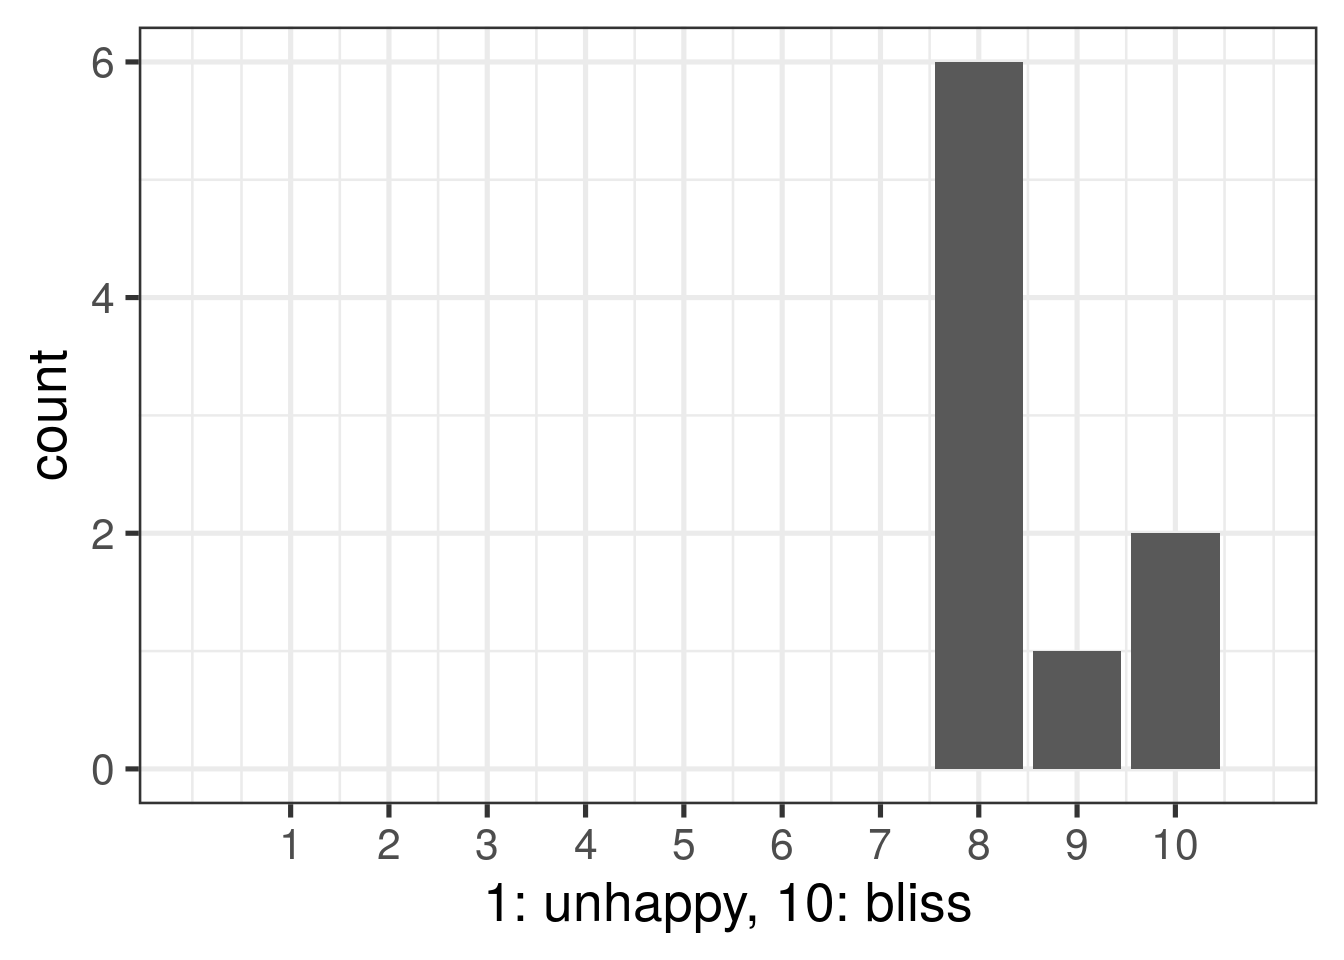
\includegraphics{_main_files/figure-latex/plot_5_2022-04-1.pdf}

\hypertarget{is-there-something-that-could-be-provided-to-make-you-happier}{%
\section{Is there something that could be provided to make you happier?}\label{is-there-something-that-could-be-provided-to-make-you-happier}}

\begin{itemize}
\tightlist
\item
  Some kind of incentive to help drive motivation and innovation would be a start
\item
  I do not wish to answer
\item
  Nothing in particular, I feel happier being a part of the team and working on different projects.
\item
  Not sure
\item
  I'm quite happy.
\item
  I am good now!
\item
  Higher salary
\item
  Just more team members because everyone has quite a lot on their plates
\item
  more computing power and storage can always help (obviously not really team related though)
\end{itemize}

\hypertarget{what-is-your-impression-of-social-life-in-the-team-too-social-not-enough-or-just-right-if-you-want-to-improve-the-social-life-in-the-lab-what-are-your-suggestions-for-achieving-this}{%
\section{What is your impression of social life in the team? Too social, not enough, or just right? If you want to improve the social life in the lab, what are your suggestions for achieving this?}\label{what-is-your-impression-of-social-life-in-the-team-too-social-not-enough-or-just-right-if-you-want-to-improve-the-social-life-in-the-lab-what-are-your-suggestions-for-achieving-this}}

\begin{itemize}
\tightlist
\item
  Somewhat more frequent happy hours or small activities could be good
\item
  I think the social life is just right
\item
  just right
\item
  Just right.
\item
  Not very social, but I think people would like for it to be more social.
\item
  Just right.
\item
  I think we could be a bit more social, I think the return of social lunch is a step in the right direction! Maybe we can try a few more after-work gatherings that aren't always alcohol centered (go get coffee, a snack, or ice-cream instead?).
\item
  It looks pretty social to me. We can probably have more social outings/hobby groups
\item
  Just right. We could maybe spend more time together if people want.
\end{itemize}

\hypertarget{how-comfortable-do-you-feel-sharing-personal-concerns-housing-financial-family-physical-or-mental-health-with-me}{%
\section{How comfortable do you feel sharing personal concerns (housing, financial, family, physical or mental health) with me?}\label{how-comfortable-do-you-feel-sharing-personal-concerns-housing-financial-family-physical-or-mental-health-with-me}}

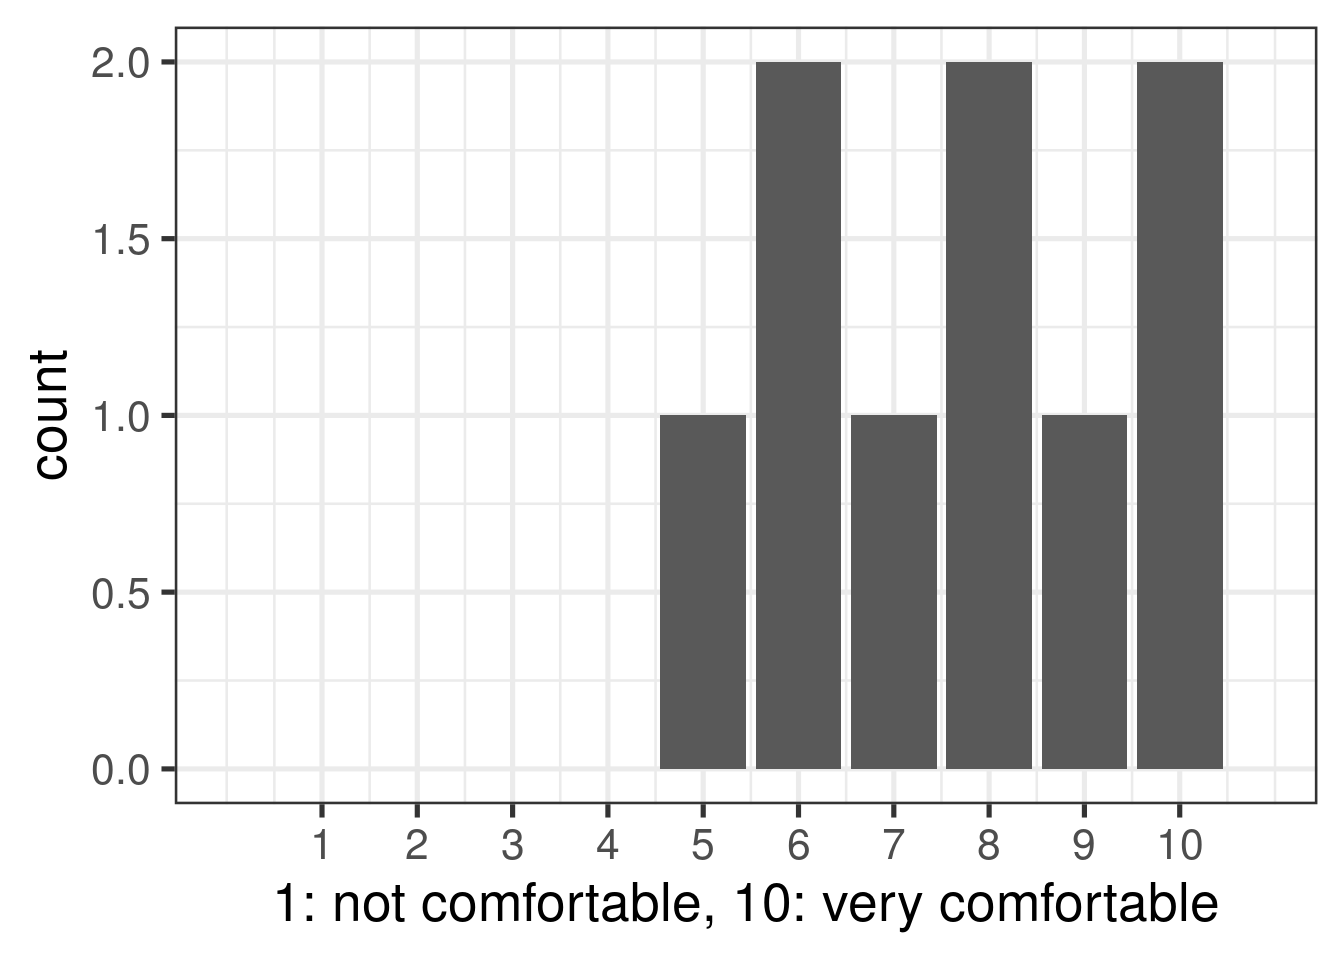
\includegraphics{_main_files/figure-latex/plot_8_2022-04-1.pdf}

\hypertarget{do-you-feel-explicit-or-implicit-pressure-to-work-more-hours-than-you-feel-is-healthy}{%
\section{Do you feel explicit or implicit pressure to work more hours than you feel is healthy?}\label{do-you-feel-explicit-or-implicit-pressure-to-work-more-hours-than-you-feel-is-healthy}}

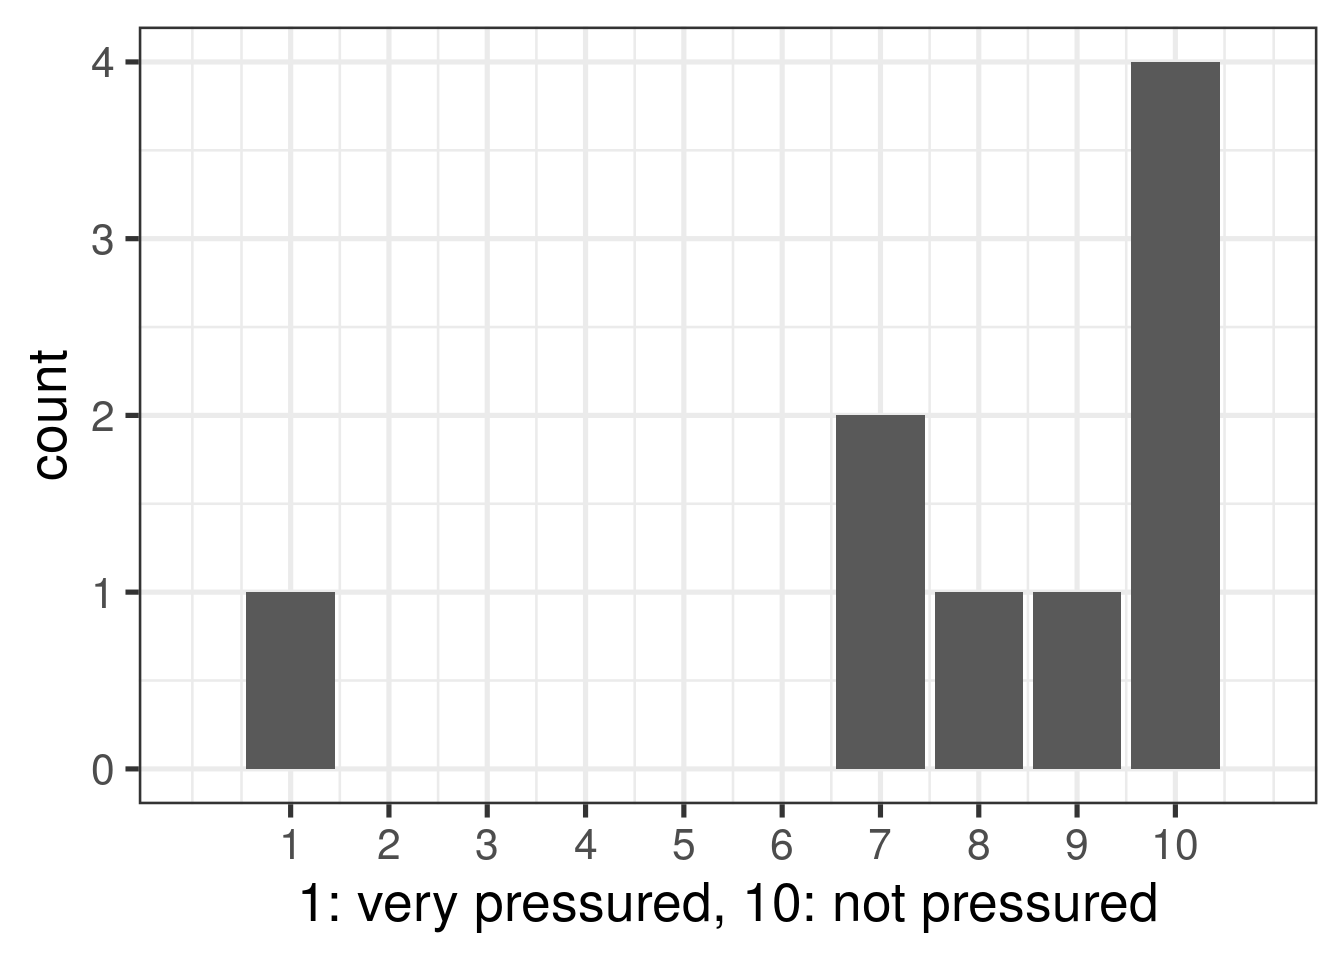
\includegraphics{_main_files/figure-latex/plot_9_2022-04-1.pdf}

\hypertarget{do-you-feel-explicit-or-implicit-pressure-to-avoid-taking-vacations}{%
\section{Do you feel explicit or implicit pressure to avoid taking vacations?}\label{do-you-feel-explicit-or-implicit-pressure-to-avoid-taking-vacations}}

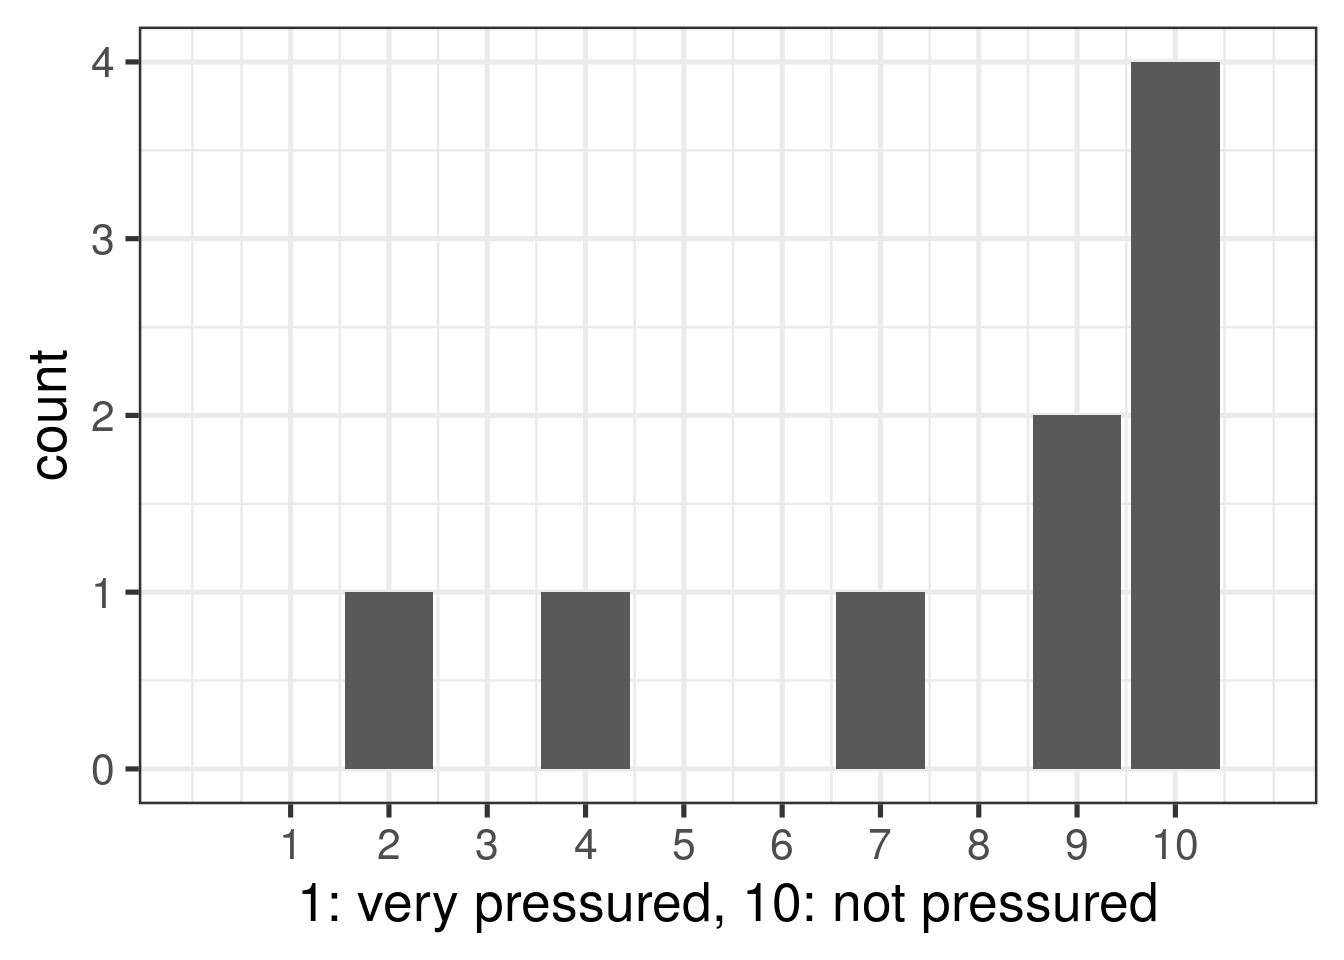
\includegraphics{_main_files/figure-latex/plot_10_2022-04-1.pdf}

\hypertarget{have-you-experienced-or-witnessed-a-hostile-work-environment-in-the-team-bullying-gender-harassment-sexual-harassment}{%
\section{Have you experienced or witnessed a hostile work environment in the team? (bullying, gender harassment, sexual harassment)}\label{have-you-experienced-or-witnessed-a-hostile-work-environment-in-the-team-bullying-gender-harassment-sexual-harassment}}

\begin{verbatim}
## Warning: Removed 1 rows containing missing values (geom_bar).
\end{verbatim}

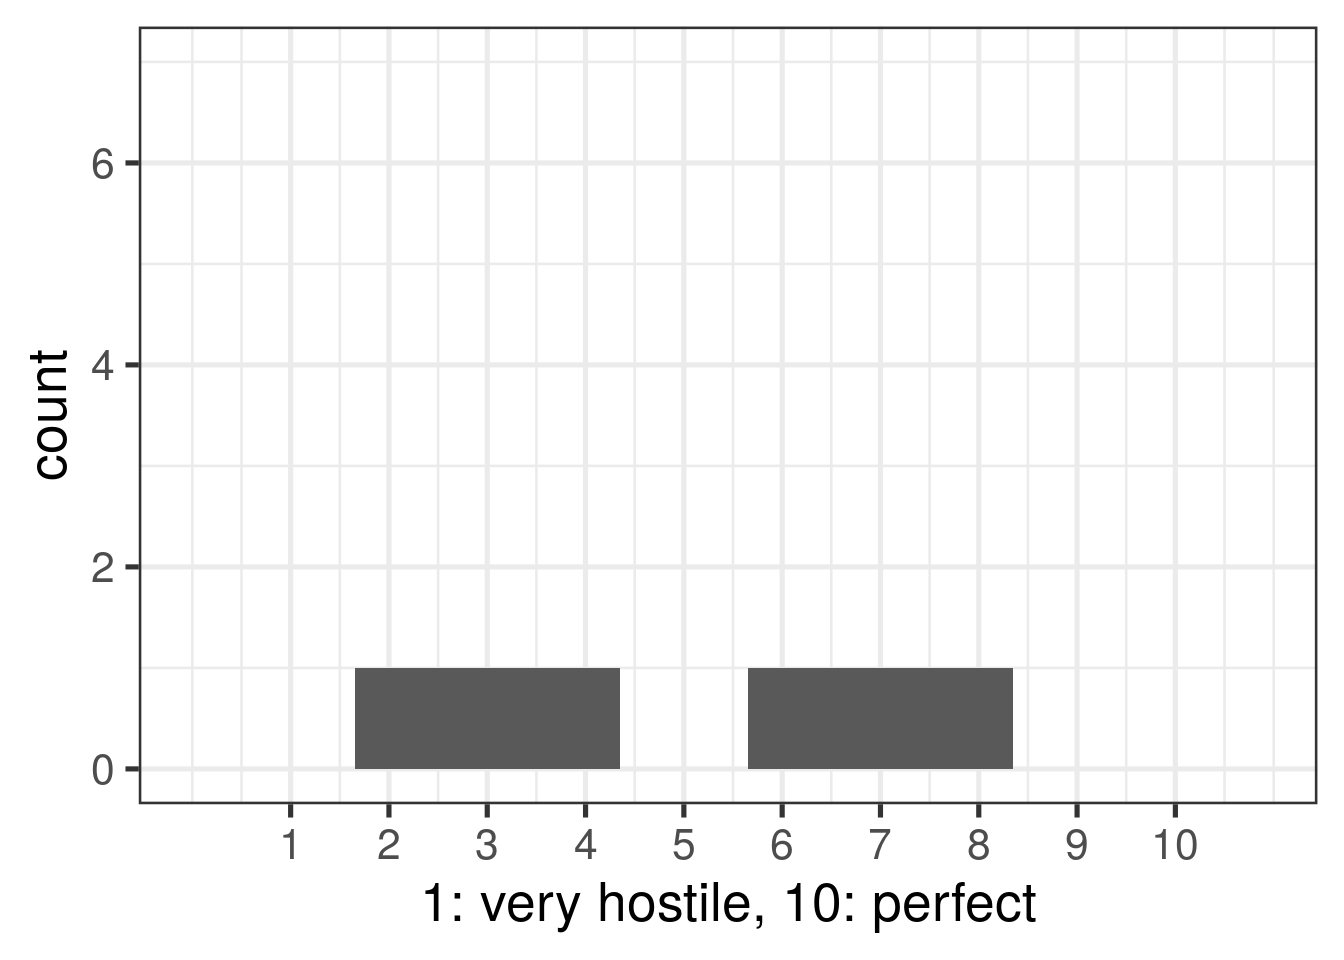
\includegraphics{_main_files/figure-latex/plot_11_2022-04-1.pdf}

\hypertarget{how-well-does-the-team-communicate-as-a-whole}{%
\section{How well does the team communicate as a whole?}\label{how-well-does-the-team-communicate-as-a-whole}}

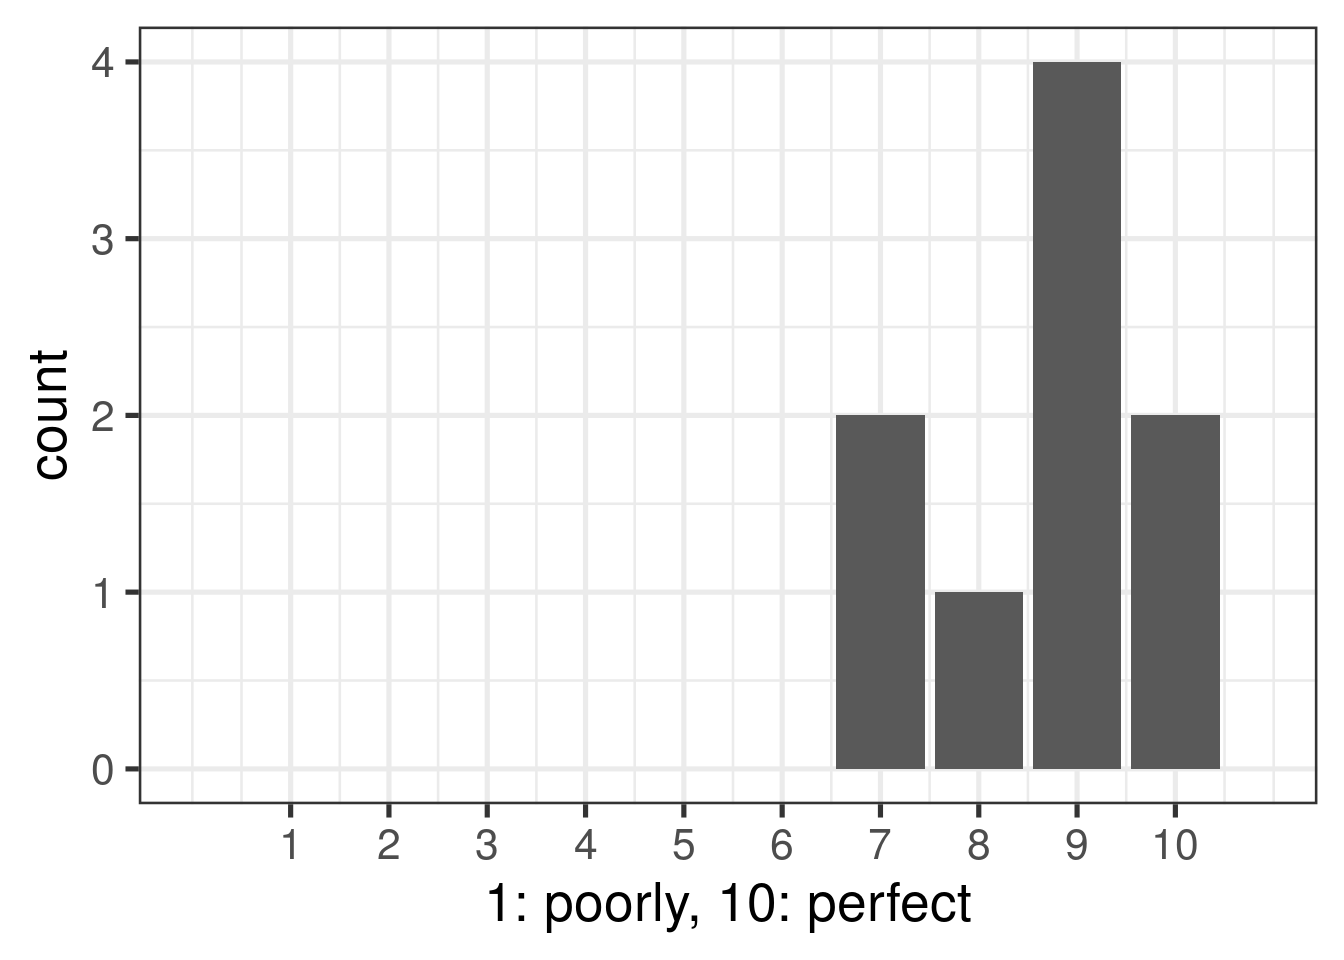
\includegraphics{_main_files/figure-latex/plot_12_2022-04-1.pdf}

\hypertarget{what-are-some-ways-that-we-could-improve-communication-in-the-team}{%
\section{What are some ways that we could improve communication in the team?}\label{what-are-some-ways-that-we-could-improve-communication-in-the-team}}

\begin{itemize}
\tightlist
\item
  Being in person could help. Also I think there's going to be more pressure on us to give services to other labs and Leo should be the point person for that. I don't like being reached out to by other PIs to ask me to do things outside my responsibilities.
\item
  It's sometimes hard to see how projects are connected or who is working on what. Team meetings that clarify this are helpful
\item
  Maybe take time (like 10 min) during the Wednesday team meetings to check in with everyone about progress on projects. It is sometimes a really long time before the cycle of presentations to get all the way around, and its nice to hear the progress people have made. This also might be a good way to make connections about similar problems/questions. Also better reminders about what is happening at the team meeting from the person going to present would be helpful for the rest of the group to prep.\\
\item
  I feel we communicate well but sometimes the important information is lost in slack messages but there has never been an issue.
\item
  Slack, Calendly, and Google doc have been very powerful, I think, to facilitate our communications.
\item
  Slack's good.
\item
  NA
\item
  weekly team meetings could include some (voluntary) sharing of work/issue updates or questions for the team, instead of the entire hour being allocated to full presentations
\item
  N/A
\end{itemize}

\hypertarget{do-you-feel-that-lab-rulespolicies-are-clear-are-there-unspoken-rules-or-policies-that-you-feel-should-be-more-clearly-communicated}{%
\section{Do you feel that lab rules/policies are clear? Are there unspoken rules or policies that you feel should be more clearly communicated?}\label{do-you-feel-that-lab-rulespolicies-are-clear-are-there-unspoken-rules-or-policies-that-you-feel-should-be-more-clearly-communicated}}

\begin{itemize}
\tightlist
\item
  N/A
\item
  They are clear, and it's not looked down upon when I want something clarified that may be super obvious to others.
\item
  As a collaborator, I don't know so much about the lab rules/policies. I wonder where I can find them, though.
\item
  Pretty Clear
\item
  Not really. I don't feel like we have many lab rules or if we do I don't know what they are.
\item
  Yes
\item
  All policies are clear.
\item
  rules are quite clear
\item
  How to handle if other PIs/groups ask for your help (something that would take more than the dsgs are designed for)?
\end{itemize}

\hypertarget{are-there-policies-you-feel-should-be-explicitly-written-if-so-please-explain-which-ones.}{%
\section{Are there policies you feel should be explicitly written? If so, please explain which ones.}\label{are-there-policies-you-feel-should-be-explicitly-written-if-so-please-explain-which-ones.}}

\begin{itemize}
\tightlist
\item
  No, I think it is pretty clear and people are helpful and understanding to explain something again.
\item
  no
\item
  N/A
\item
  I think it's important to have clear policies about authorship and division of work on projects.
\item
  No
\item
  Not currently
\item
  NA
\item
  N/A
\item
  No
\end{itemize}

\hypertarget{do-you-feel-that-the-same-rules-apply-to-everyone-in-team-if-not-please-explain.}{%
\section{Do you feel that the same rules apply to everyone in team? If not, please explain.}\label{do-you-feel-that-the-same-rules-apply-to-everyone-in-team-if-not-please-explain.}}

\begin{itemize}
\tightlist
\item
  yes
\item
  Yes, no injustice or favoritism
\item
  Yes
\item
  Yes, but equitably
\item
  yes
\item
  N/A
\item
  Yes
\item
  Yes
\item
  Yes
\end{itemize}

\hypertarget{do-you-feel-empowered-to-make-suggestions-to-me-to-improve-the-team-culture-organization}{%
\section{Do you feel empowered to make suggestions to me to improve the team culture/ organization?}\label{do-you-feel-empowered-to-make-suggestions-to-me-to-improve-the-team-culture-organization}}

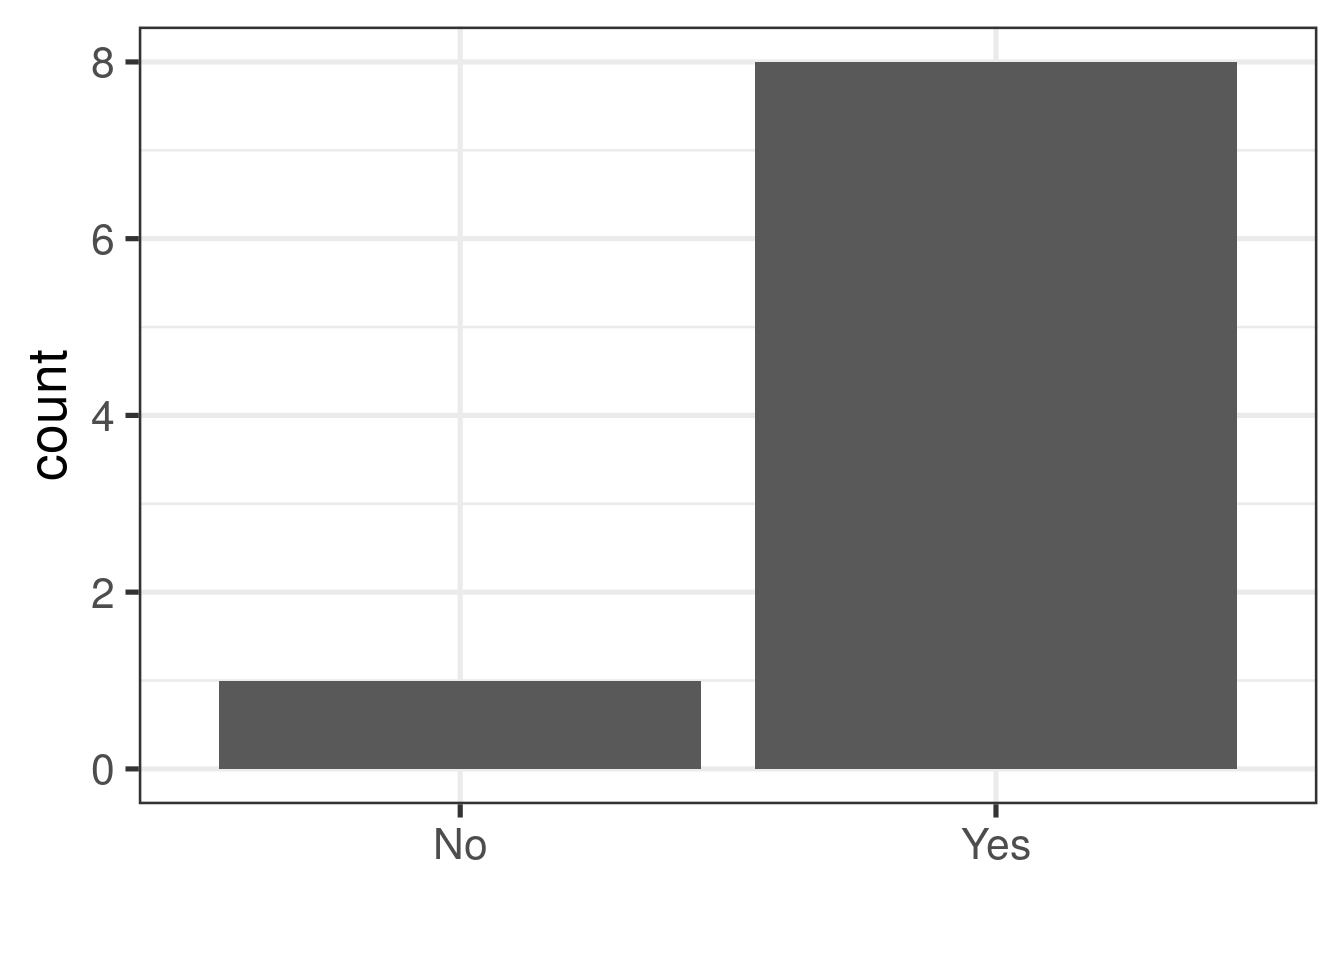
\includegraphics{_main_files/figure-latex/plot_17_2022-04-1.pdf}

\hypertarget{do-you-feel-empowered-to-make-suggestions-to-your-colleagues-to-improve-the-team-culture-organization}{%
\section{Do you feel empowered to make suggestions to your colleagues to improve the team culture/ organization?}\label{do-you-feel-empowered-to-make-suggestions-to-your-colleagues-to-improve-the-team-culture-organization}}

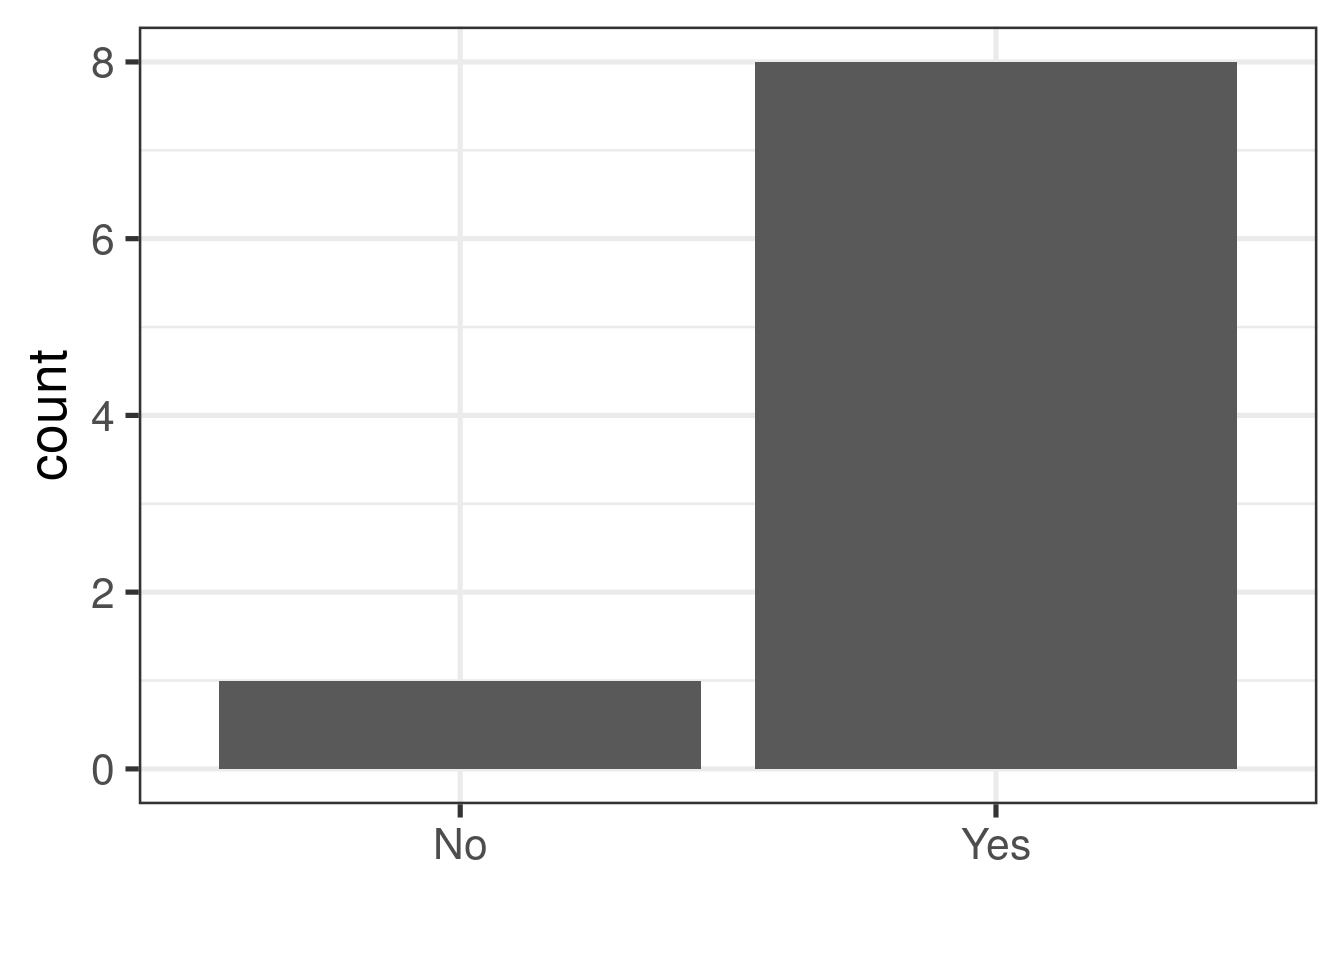
\includegraphics{_main_files/figure-latex/plot_18_2022-04-1.pdf}

\hypertarget{if-you-do-not-feel-empowered-to-make-suggestions-to-your-colleagues-in-the-team-or-to-me-to-improve-the-team-culture-organization-please-tell-me-more-about-this.}{%
\section{If you do not feel empowered to make suggestions to your colleagues in the team or to me to improve the team culture/ organization, please tell me more about this.}\label{if-you-do-not-feel-empowered-to-make-suggestions-to-your-colleagues-in-the-team-or-to-me-to-improve-the-team-culture-organization-please-tell-me-more-about-this.}}

\begin{itemize}
\tightlist
\item
  I said yes to both questions :)
\item
  n/a
\item
  NA
\item
  N/A
\item
  na
\item
  I feel empowered to suggest changes.
\item
  I don't really feel comfortable providing negative feedback about the team.
\item
  N/A
\item
  Yes
\end{itemize}

\hypertarget{do-you-feel-you-have-enough-feedback-on-your-project}{%
\section{Do you feel you have enough feedback on your project?}\label{do-you-feel-you-have-enough-feedback-on-your-project}}

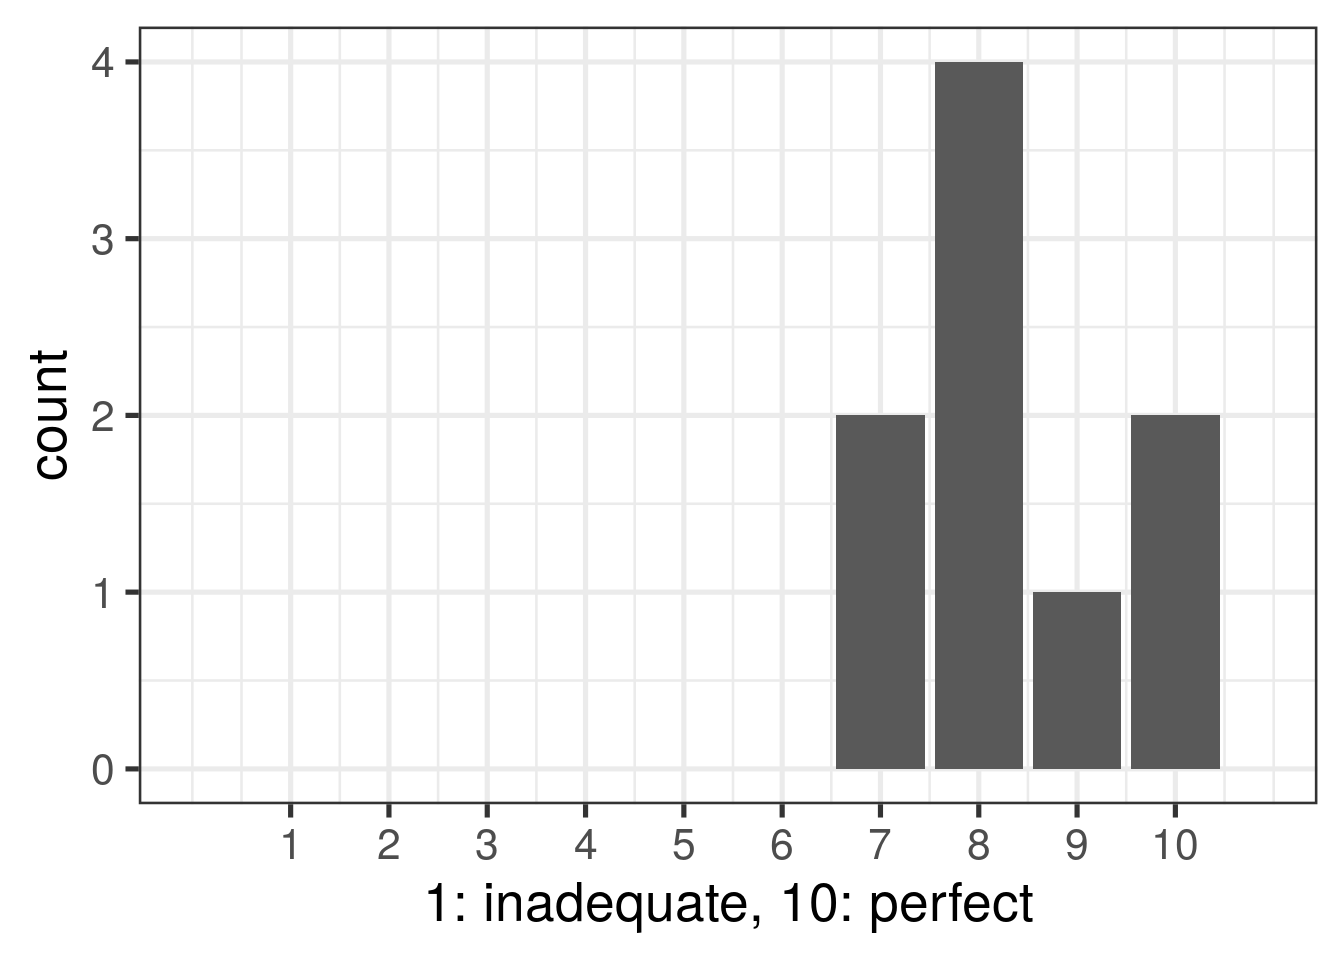
\includegraphics{_main_files/figure-latex/plot_20_2022-04-1.pdf}

\hypertarget{do-you-feel-you-have-enough-time-to-meet-with-me}{%
\section{Do you feel you have enough time to meet with me?}\label{do-you-feel-you-have-enough-time-to-meet-with-me}}

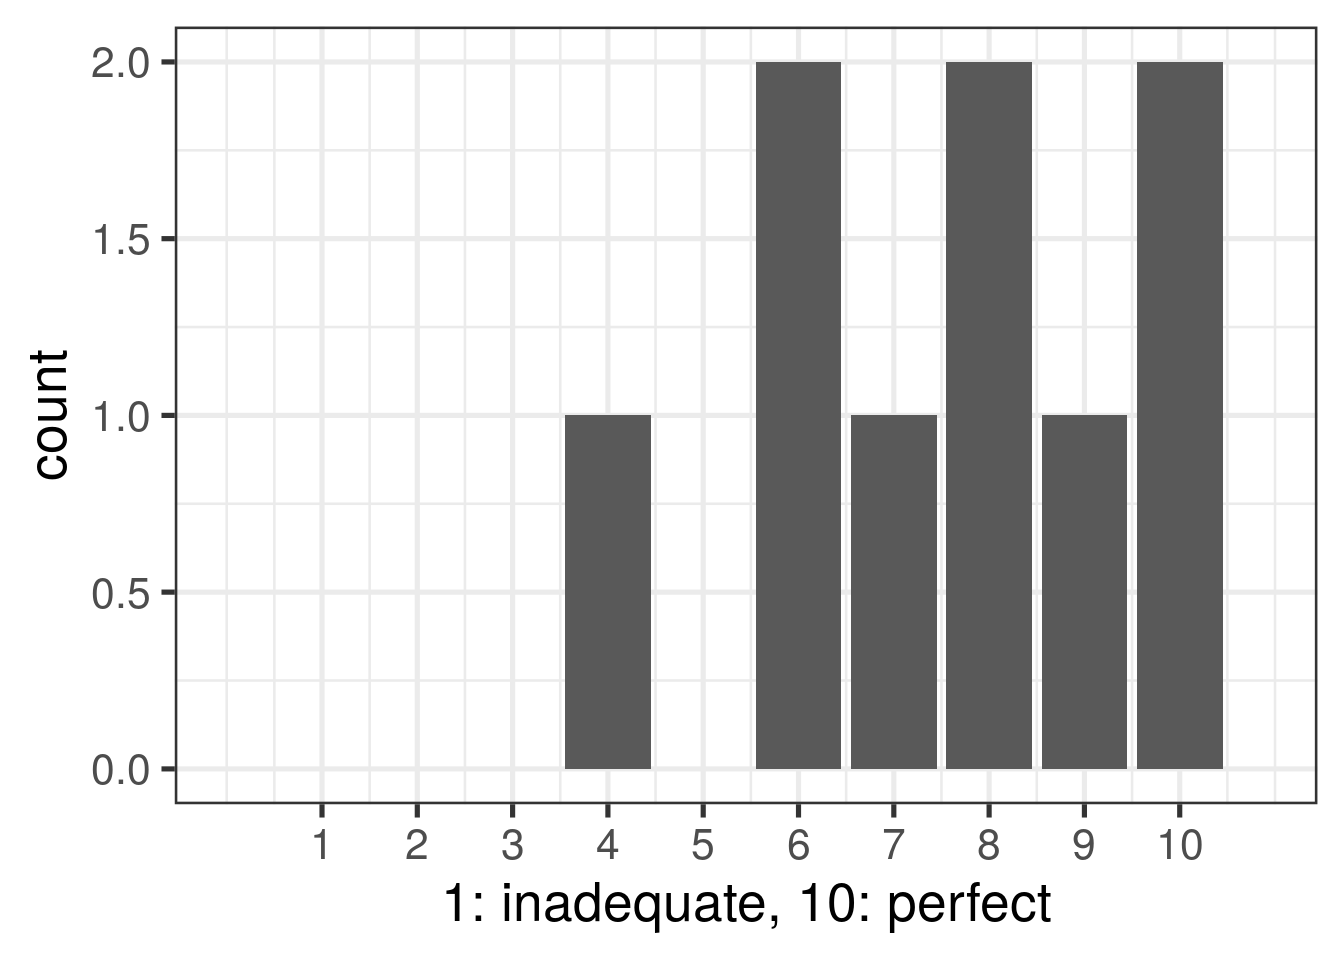
\includegraphics{_main_files/figure-latex/plot_21_2022-04-1.pdf}

\hypertarget{how-useful-do-you-find-one-on-one-meetings-with-me}{%
\section{How useful do you find one-on-one meetings with me?}\label{how-useful-do-you-find-one-on-one-meetings-with-me}}

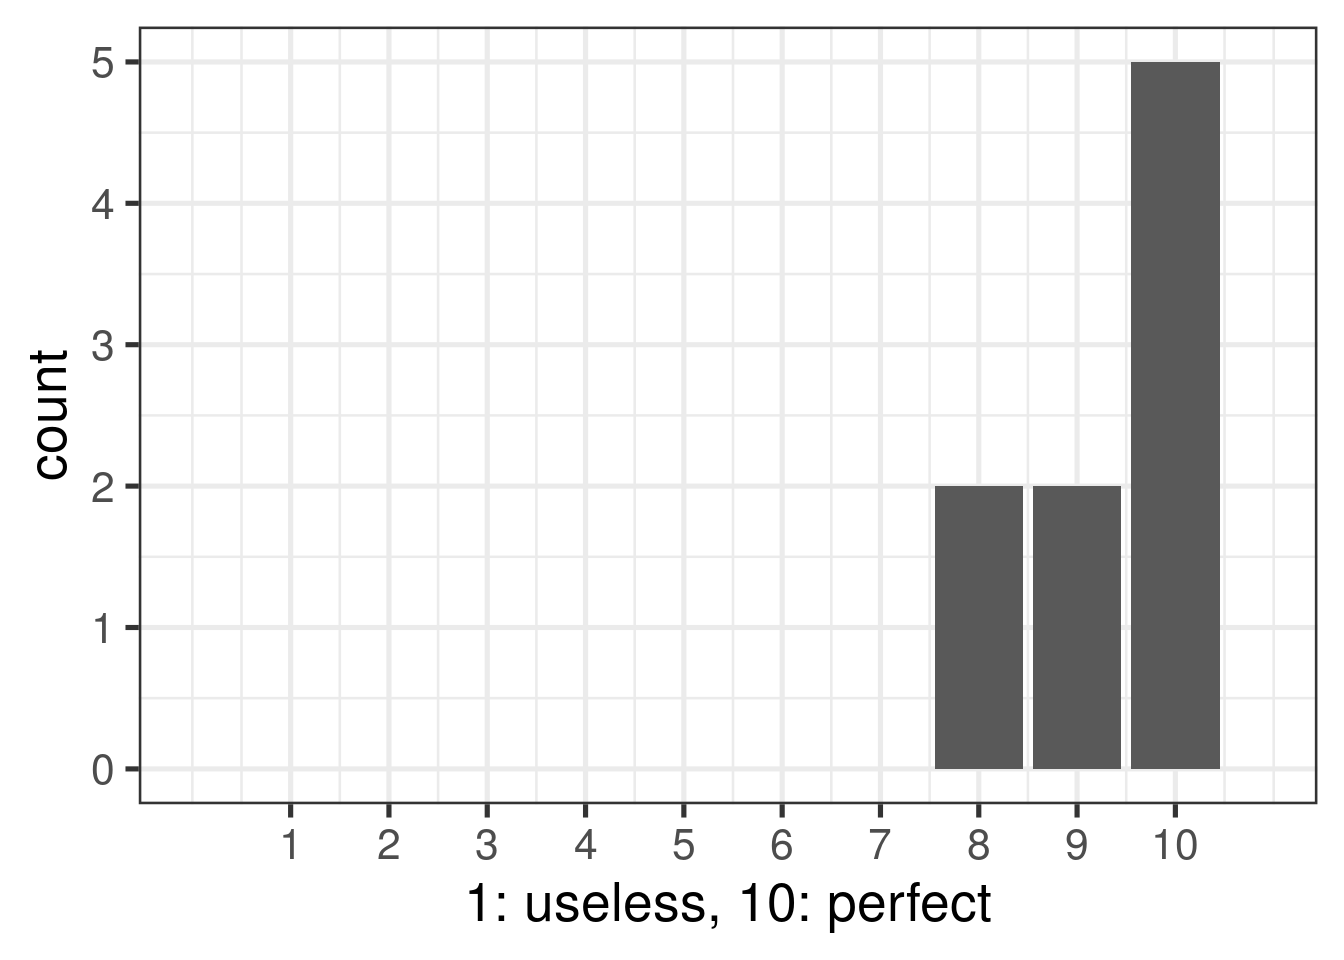
\includegraphics{_main_files/figure-latex/plot_22_2022-04-1.pdf}

\hypertarget{is-there-something-that-could-make-these-meetings-more-useful-or-productive}{%
\section{Is there something that could make these meetings more useful or productive?}\label{is-there-something-that-could-make-these-meetings-more-useful-or-productive}}

\begin{itemize}
\tightlist
\item
  Maybe try to have agenda items on paper or the screen, so we don't go off too far on tangents
\item
  na
\item
  There was a stretch this year where a lot of meetings got canceled and it made things very hard to manage.
\item
  planning my own questions better and improving my own communication skills
\item
  N/A
\item
  These meetings are pretty useful, understanding the background/purpose of what one is doing and why makes it easier to understand things. So maybe a background in the beginning would be more helpful.
\item
  Could spend more time going over code for important analysis
\item
  No.~I really like being able to record the meetings and watch them again.
\item
  I think we've been using the meetings very efficiently and time-efficiently. The way Leo is assigning issues to assignees at the end of meeting also works very well, I think.
\end{itemize}

\hypertarget{do-you-think-the-current-system-of-formal-scheduled-weekly-one-on-one-meetings-is-working-should-these-be-less-frequent-more-frequent-or-stay-as-is}{%
\section{Do you think the current system of formal scheduled weekly one-on-one meetings is working? Should these be less frequent, more frequent, or stay as is?}\label{do-you-think-the-current-system-of-formal-scheduled-weekly-one-on-one-meetings-is-working-should-these-be-less-frequent-more-frequent-or-stay-as-is}}

\begin{itemize}
\tightlist
\item
  Stay as is
\item
  I think they're good as they are.
\item
  This frequency is good in combination with weekly project-specific meetings.
\item
  They can stay as-is
\item
  fine as is
\item
  stay as is
\item
  The current system work well for me. I think that the Monday meetings are very helpful for me planning my week! I also feel like we make one-on-one meetings work when more are needed.
\item
  Between `stay as is' and `more frequent': depending on the pace of work/progress
\item
  stay as is.
\end{itemize}

\hypertarget{do-you-think-you-would-benefit-from-more-formal-feedback-on-your-progress}{%
\section{Do you think you would benefit from more formal feedback on your progress?}\label{do-you-think-you-would-benefit-from-more-formal-feedback-on-your-progress}}

\begin{itemize}
\tightlist
\item
  not sure
\item
  No, the current amount works fine
\item
  yes
\item
  Sure, I sometimes feel like I could benefit from code review, especially for ``by the book'' type analysis.
\item
  Yes, formal and honest feedback always helps.
\item
  yes
\item
  Yes!
\item
  Yes
\item
  No
\end{itemize}

\hypertarget{how-supported-do-you-feel-by-me-and-do-you-think-that-you-are-getting-the-mentoring-career-advice-and-general-guidance-to-succeed}{%
\section{How supported do you feel by me, and do you think that you are getting the mentoring, career advice, and general guidance to succeed?}\label{how-supported-do-you-feel-by-me-and-do-you-think-that-you-are-getting-the-mentoring-career-advice-and-general-guidance-to-succeed}}

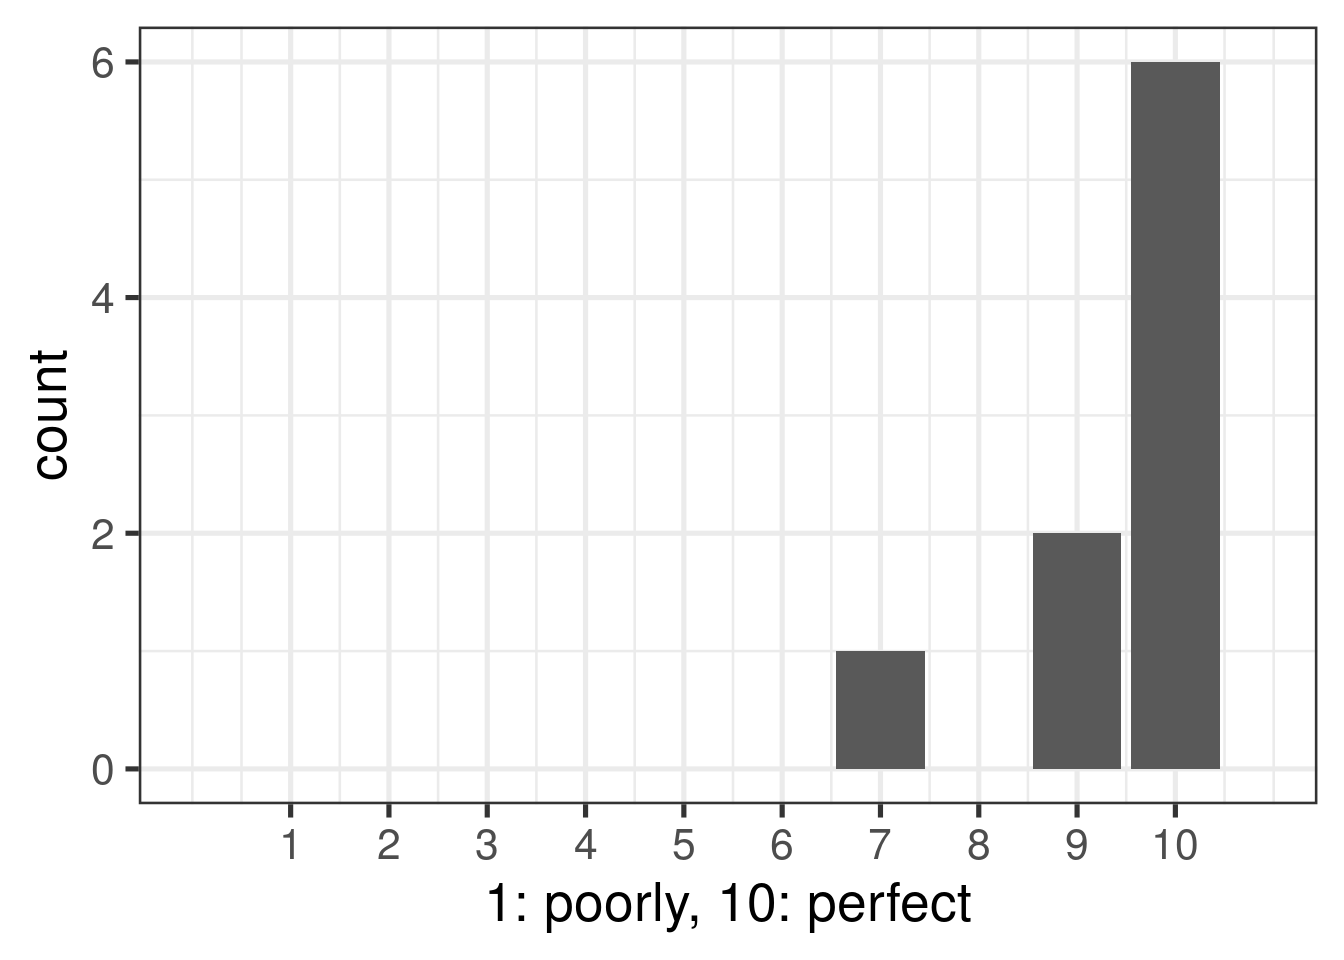
\includegraphics{_main_files/figure-latex/plot_26_2022-04-1.pdf}

\hypertarget{do-you-want-formal-training-in-giving-talks}{%
\section{Do you want formal training in giving talks?}\label{do-you-want-formal-training-in-giving-talks}}

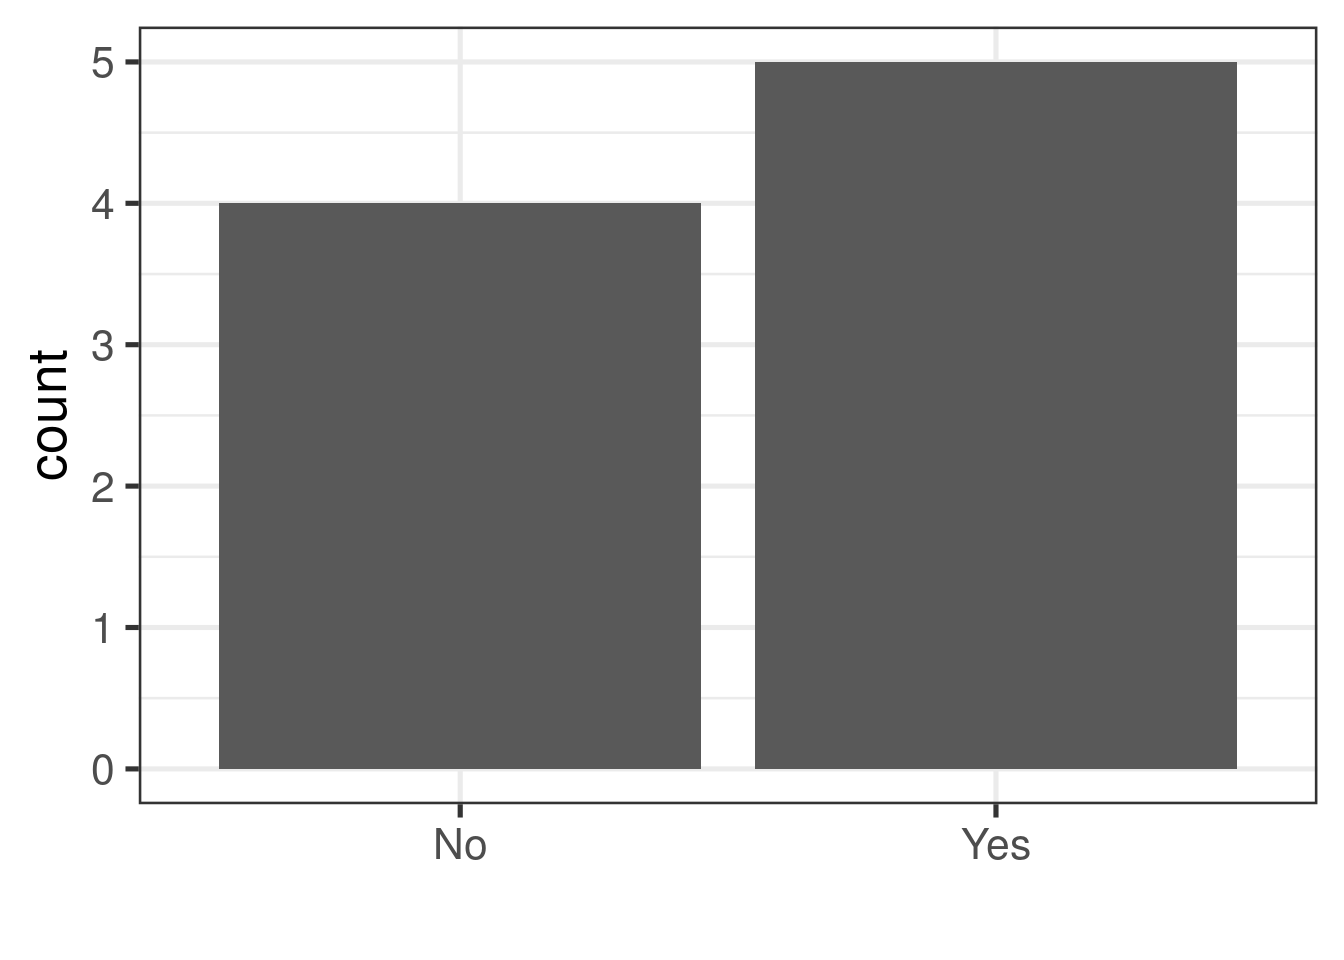
\includegraphics{_main_files/figure-latex/plot_27_2022-04-1.pdf}

\hypertarget{do-you-want-to-have-an-annual-mentoring-meeting-to-go-over-your-individual-development-plan-and-discuss-post-phd-or-post-postdoc-plans-leo-edit-see-httpslcolladotor.github.iobioc_team_dscareer-growth.html.}{%
\section{\texorpdfstring{Do you want to have an Annual Mentoring Meeting to go over your Individual Development Plan and discuss post-PhD or post-Postdoc plans? Leo edit: see \url{https://lcolladotor.github.io/bioc_team_ds/career-growth.html}.}{Do you want to have an Annual Mentoring Meeting to go over your Individual Development Plan and discuss post-PhD or post-Postdoc plans? Leo edit: see https://lcolladotor.github.io/bioc\_team\_ds/career-growth.html.}}\label{do-you-want-to-have-an-annual-mentoring-meeting-to-go-over-your-individual-development-plan-and-discuss-post-phd-or-post-postdoc-plans-leo-edit-see-httpslcolladotor.github.iobioc_team_dscareer-growth.html.}}

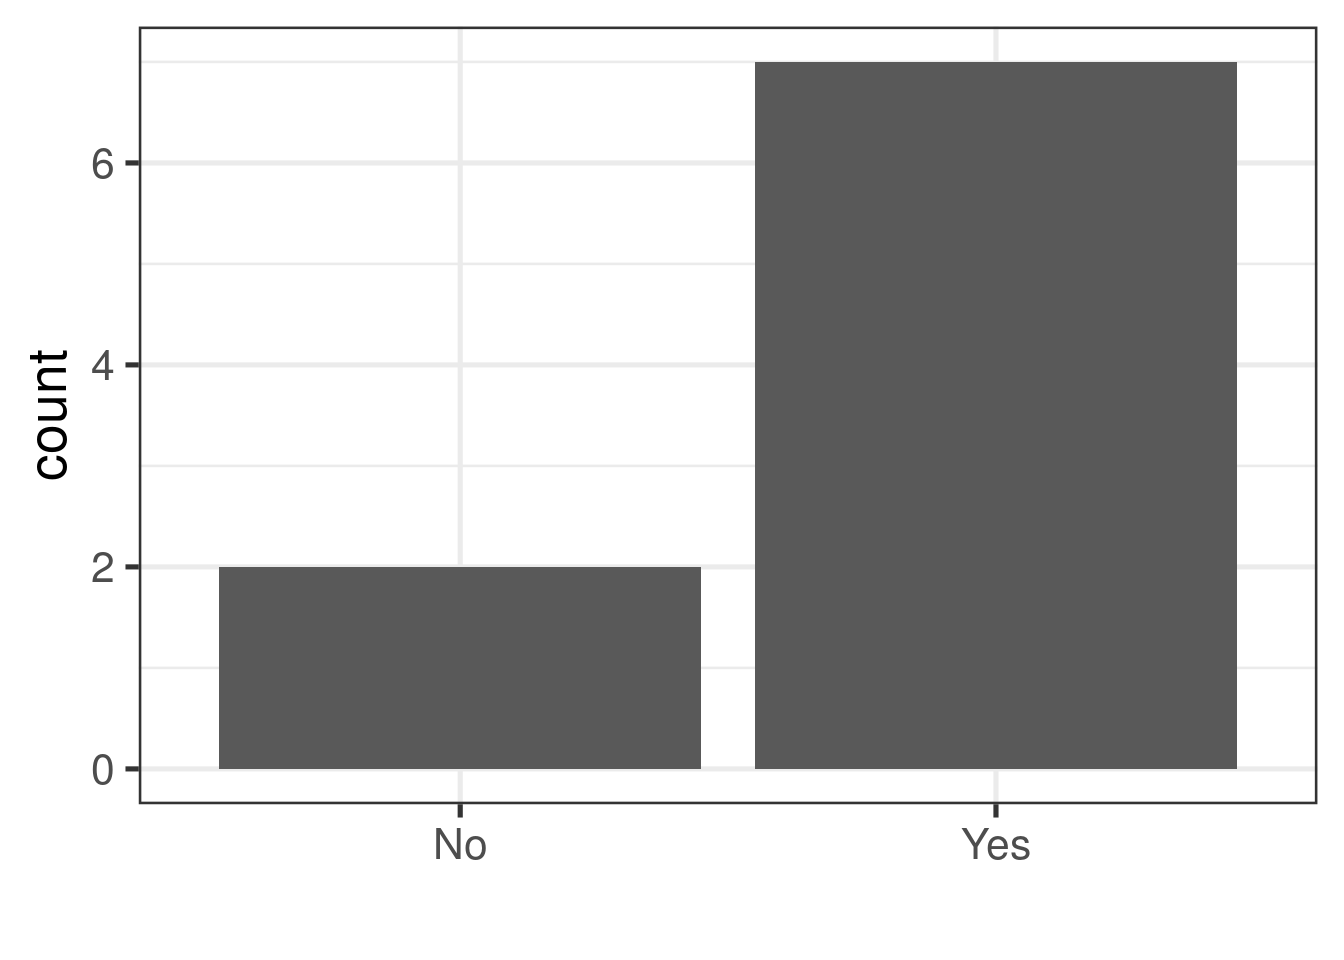
\includegraphics{_main_files/figure-latex/plot_28_2022-04-1.pdf}

\hypertarget{what-kind-of-advice-or-information-would-be-useful-to-discuss-at-such-an-annual-mentoring-meeting}{%
\section{What kind of advice or information would be useful to discuss at such an Annual Mentoring Meeting?}\label{what-kind-of-advice-or-information-would-be-useful-to-discuss-at-such-an-annual-mentoring-meeting}}

\begin{itemize}
\tightlist
\item
  N/A
\item
  Pointing how which skills or areas of knowledge need to be improved.
\item
  Maybe resources as to what kinds of jobs/trajectories others in computational biology typically experience, so we feel more familiar and connected with the bigger data science world
\item
  n/a
\item
  Going over the progress, talking about how to constantly keep improving and getting better at what you do, opportunities to branch out based on one's interest
\item
  Given the raises and past experience with the annual review I don't see much point. I met my goals last year and still got a bad raise.
\item
  General future career plans and how current projects at LIBD are helpful for long-term goals
\item
  What are the different types of career paths that can be taken for someone in Comp Bio and how does one prepare for these paths?
\item
  Career planning, milestones to hit for advancement at LIBD. Conferences, workshops, or other opportunities I should have on the radar.
\end{itemize}

\hypertarget{do-you-have-any-explicit-feedback-on-how-i-can-improve-my-mentoring-style}{%
\section{Do you have any explicit feedback on how I can improve my mentoring style?}\label{do-you-have-any-explicit-feedback-on-how-i-can-improve-my-mentoring-style}}

\begin{itemize}
\tightlist
\item
  So far, Leo has been a great mentor. I don't have anything specific/constructive in my mind. But, I think I can talk more about this as I am interacting with Leo more often :)
\item
  no
\item
  You're awesome.
\item
  No, please continue to be the best mentor
\item
  N/A
\item
  No
\item
  Seems to be fine
\item
  NA
\item
  Not really!
\end{itemize}

\hypertarget{do-you-feel-it-is-easy-to-get-information-from-me}{%
\section{Do you feel it is easy to get information from me?}\label{do-you-feel-it-is-easy-to-get-information-from-me}}

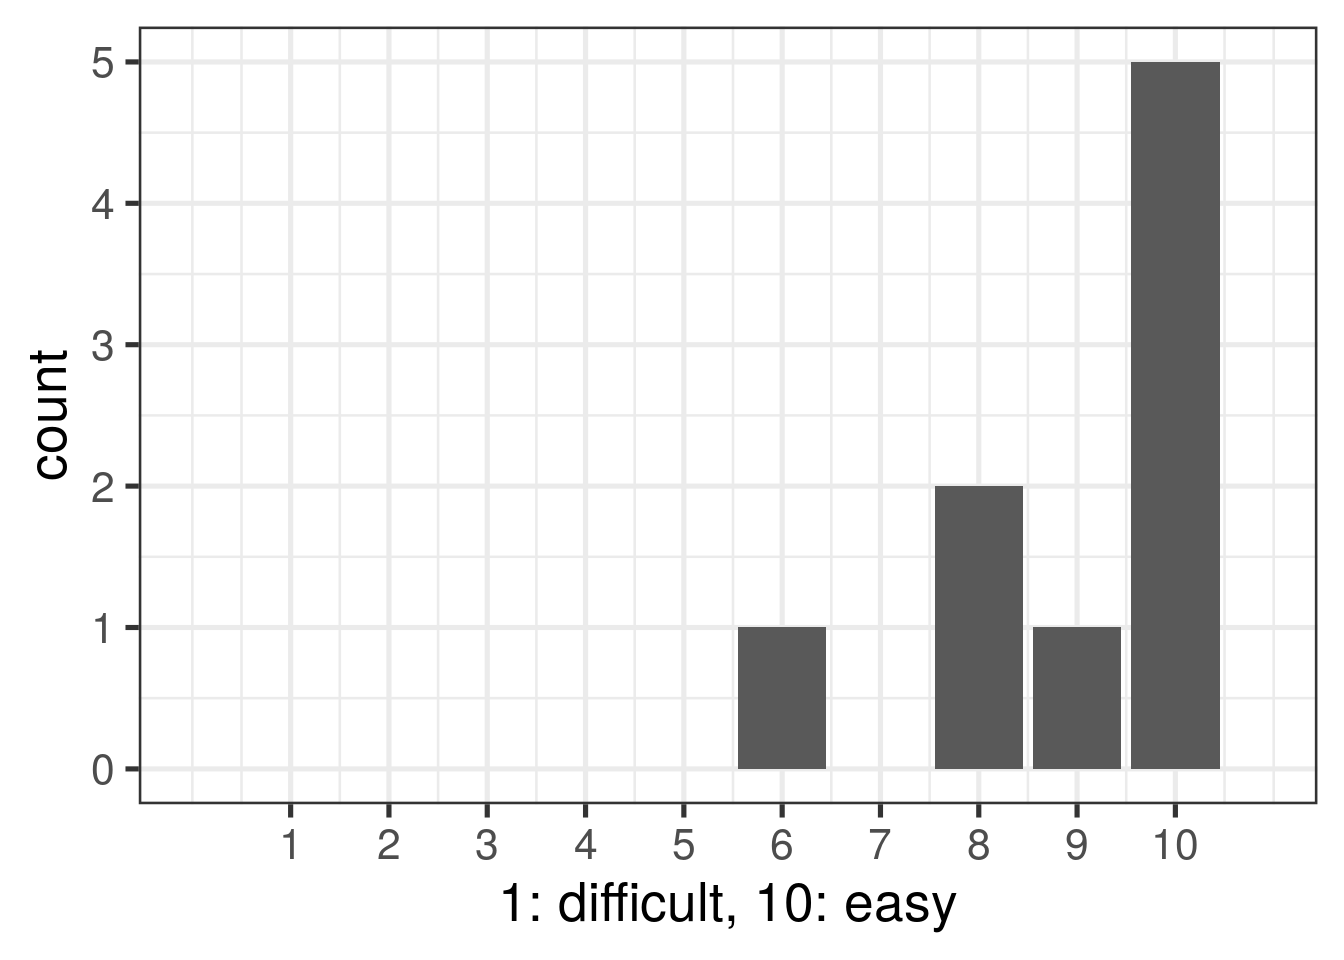
\includegraphics{_main_files/figure-latex/plot_31_2022-04-1.pdf}

\hypertarget{do-you-feel-it-is-easy-to-get-information-from-other-people-in-the-team}{%
\section{Do you feel it is easy to get information from other people in the team?}\label{do-you-feel-it-is-easy-to-get-information-from-other-people-in-the-team}}

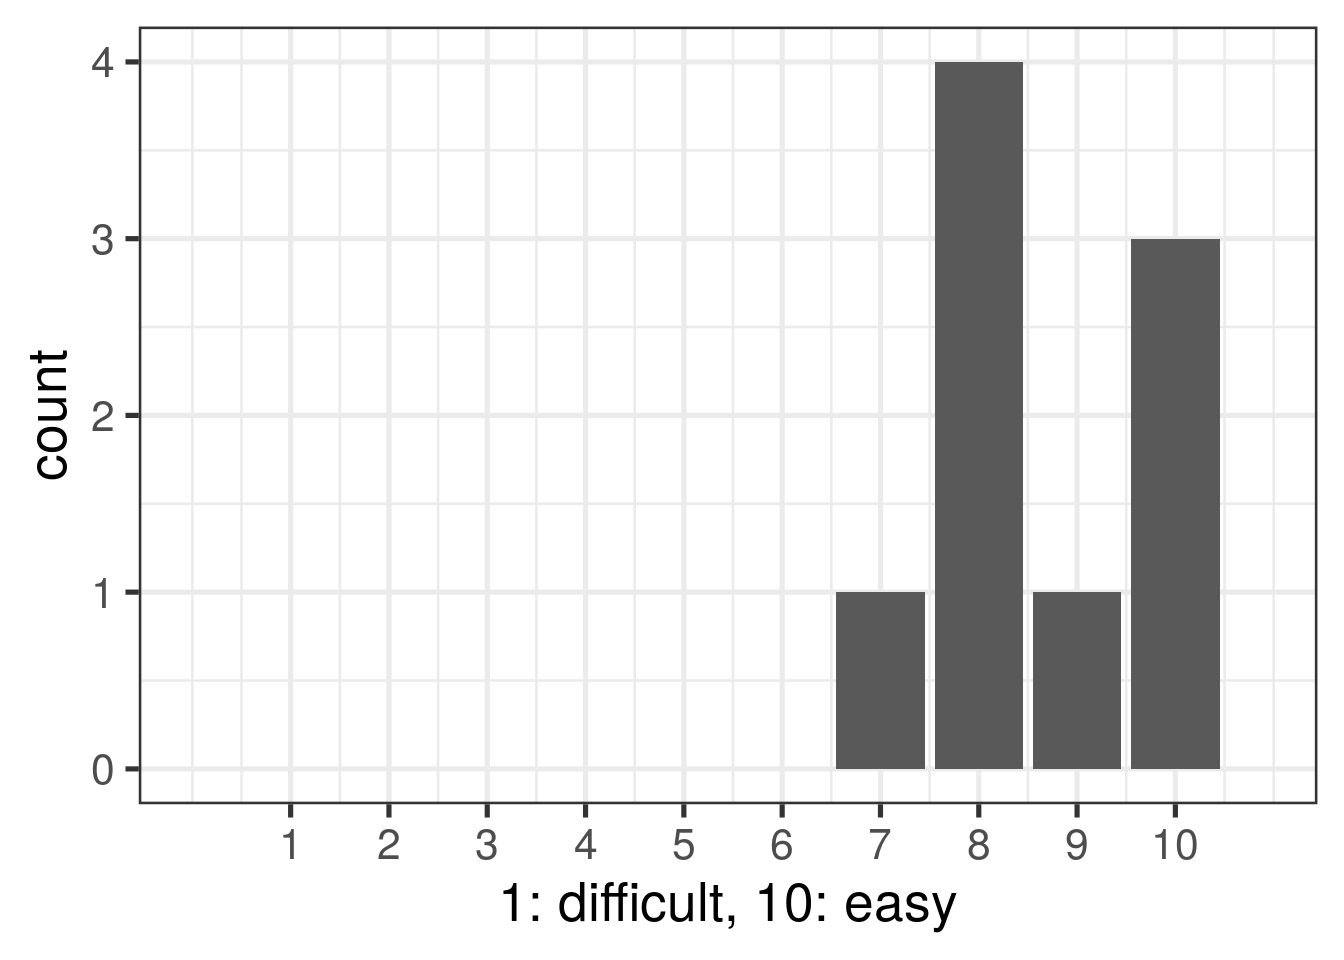
\includegraphics{_main_files/figure-latex/plot_32_2022-04-1.pdf}

\hypertarget{how-useful-do-you-find-team-meetings}{%
\section{How useful do you find team meetings?}\label{how-useful-do-you-find-team-meetings}}

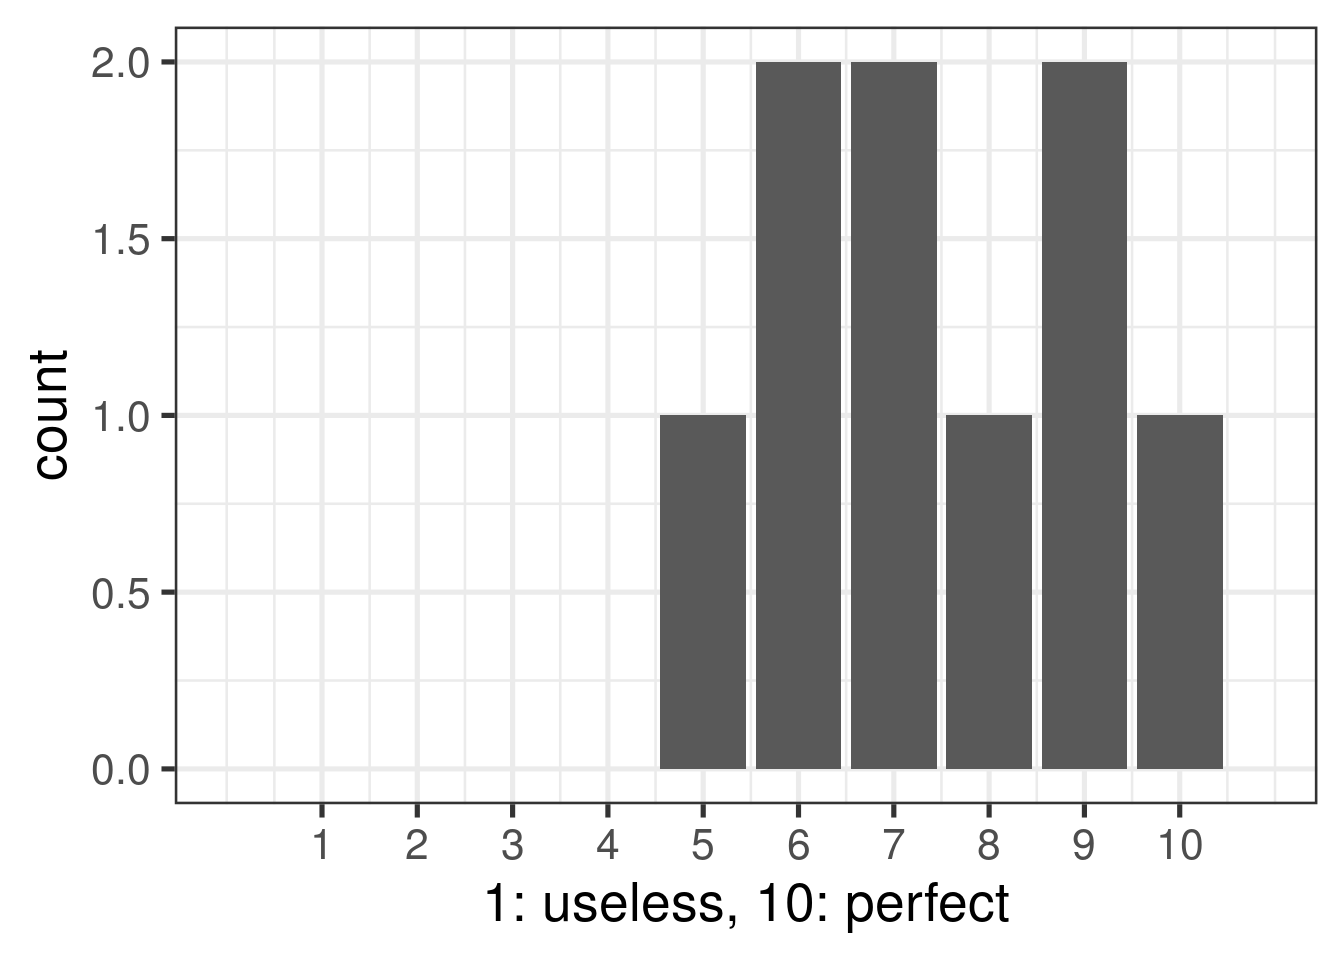
\includegraphics{_main_files/figure-latex/plot_33_2022-04-1.pdf}

\hypertarget{is-there-something-that-could-make-team-meetings-more-useful-or-productive}{%
\section{Is there something that could make team meetings more useful or productive?}\label{is-there-something-that-could-make-team-meetings-more-useful-or-productive}}

\begin{itemize}
\tightlist
\item
  N/A
\item
  Cannot say much as I do not participate in the weekly team meetings. But maybe going over some basics as we work with different people who have different levels of computational knowledge. Going over the basics in brief will help everyone come to the same a page.
\item
  There are tons of projects happening which can be hard to keep track of when you're not a part of them. Maybe we can have a google doc or website where each team shares a few resources for people to take a look at and get a better idea of what is happening if a project sounds interesting to them.
\item
  Not sure
\item
  I feel like Wednesday team meeting has mostly been replaced with journal club/individual presentations, would be good to sections out time to discuss work/progress/general concerns that the team has.
\item
  Not really
\item
  perhaps team meetings could benefit from 10-15 min of (voluntary) updates or raising any team or work related concerns, instead of the entire hour being allocated to full presentations or code sharing etc. from a single person
\item
  Sorry, since I don't participate in Leo's team meetings, I don't think I can answer this question.
\item
  I feel like meetings at the institute could benefit as a whole from having an agenda
\end{itemize}

\hypertarget{how-useful-do-you-find-sub-group-meetings}{%
\section{How useful do you find sub-group meetings?}\label{how-useful-do-you-find-sub-group-meetings}}

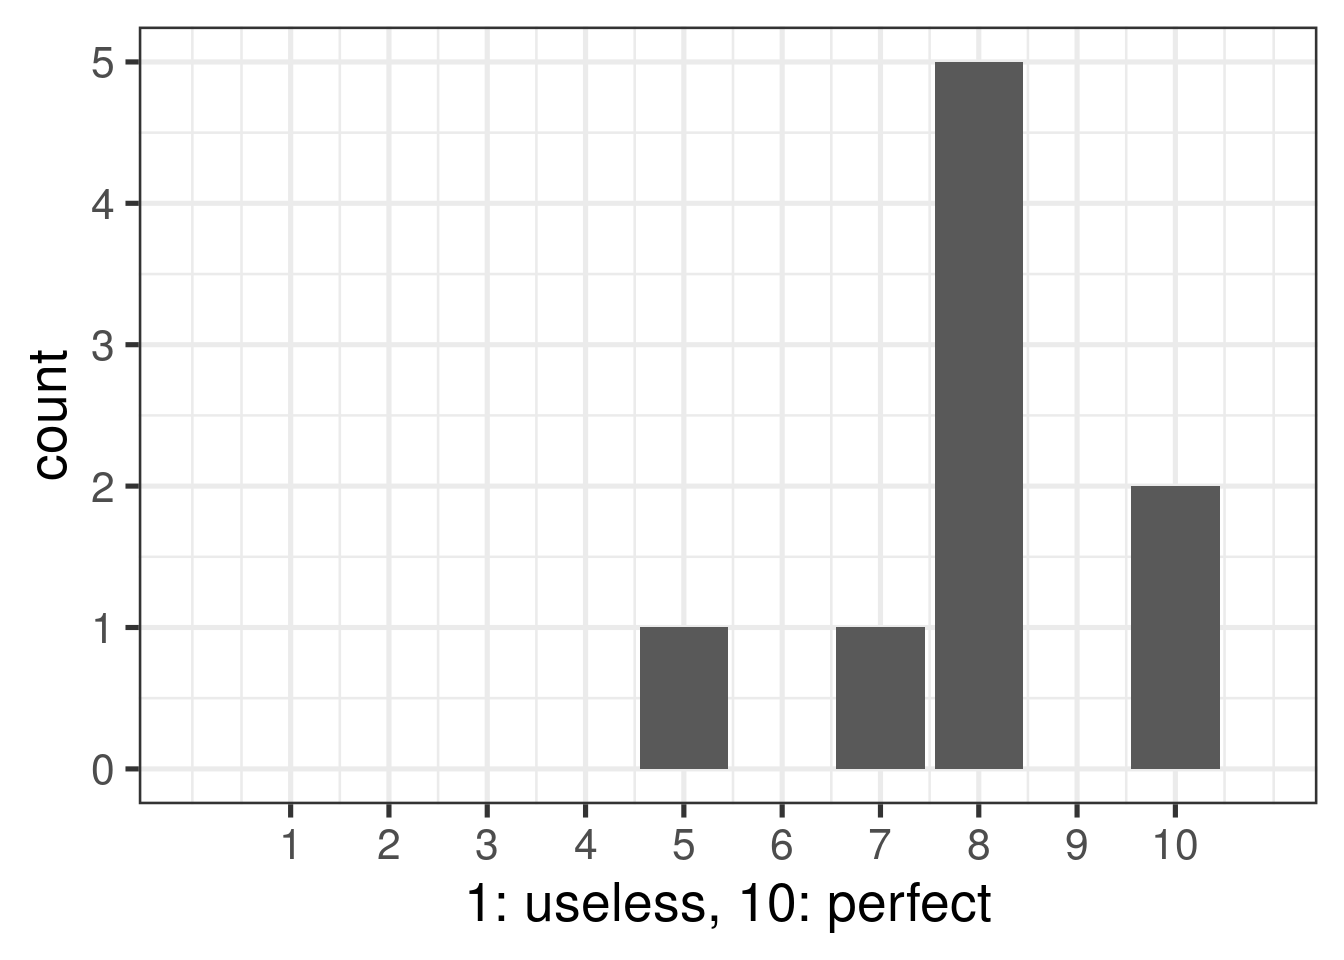
\includegraphics{_main_files/figure-latex/plot_35_2022-04-1.pdf}

\hypertarget{is-there-something-that-could-make-sub-group-meetings-more-useful-or-productive}{%
\section{Is there something that could make sub-group meetings more useful or productive?}\label{is-there-something-that-could-make-sub-group-meetings-more-useful-or-productive}}

\begin{itemize}
\tightlist
\item
  N/A
\item
  Group meetings are really helpful when they're among people that are working on very closely related projects. However, in many of the meetings there are too many people. I think the smaller the group meeting, the more productive it is.
\item
  A lot of people will still have meetings without giving much to prep with.
\item
  No, stay as it is.
\item
  Sorry, I don't get what sub-group meetings are.
\item
  some of these sub-group meetings could be replaced by asynchronous communication in writing - by Slack or email
\item
  No
\item
  na. Sometimes we end up doing things in our meeting that are different from my expectations/agenda. That tends to throw me off a bit, but perhaps it's the nature of the work.
\item
  More frequently developing an agenda (especially if multiple groups have updates/work to present)
\end{itemize}

\hypertarget{how-useful-do-you-find-the-journal-club}{%
\section{How useful do you find the journal club?}\label{how-useful-do-you-find-the-journal-club}}

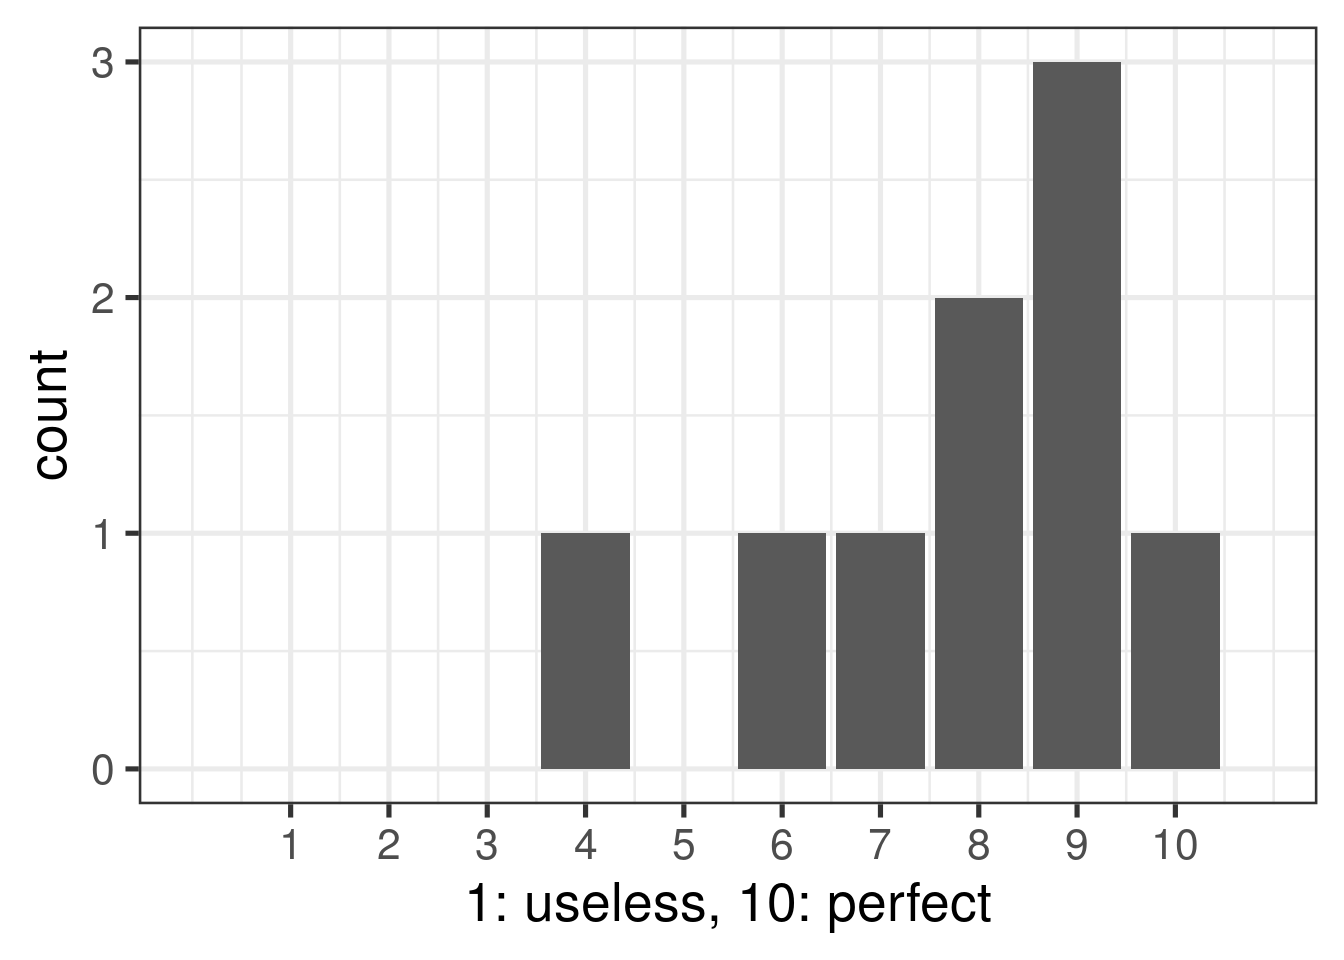
\includegraphics{_main_files/figure-latex/plot_37_2022-04-1.pdf}

\hypertarget{is-there-something-that-could-make-the-journal-club-more-useful-or-productive}{%
\section{Is there something that could make the journal club more useful or productive?}\label{is-there-something-that-could-make-the-journal-club-more-useful-or-productive}}

\begin{itemize}
\tightlist
\item
  I wonder if we can have it in a smaller group for those who are not as extraverted. Having it in a spatial group meeting is sometimes overwhelming.
\item
  no
\item
  Maybe talk about how useful the journal club tools or packages are for our data.
\item
  I think journal club should only be done in sub-group meetings
\item
  There was talk of reviewing ``classic'' bioinformatics methods papers, but that has not happened yet. Choosing papers that are more relevant to everyone in the core group would make this more engaging and worth-wile. Also making sure paper presentations are the correct length/scope.
\item
  More discussion based
\item
  N/A
\item
  If we have a Q\&A session where each person attending is encouraged to ask a question, or maybe just post a question on slack, then that's more incentive to read the paper.
\item
  N/A
\end{itemize}

\hypertarget{how-much-freedom-do-you-feel-you-have-to-decide-how-you-do-your-work}{%
\section{How much freedom do you feel you have to decide how you do your work?}\label{how-much-freedom-do-you-feel-you-have-to-decide-how-you-do-your-work}}

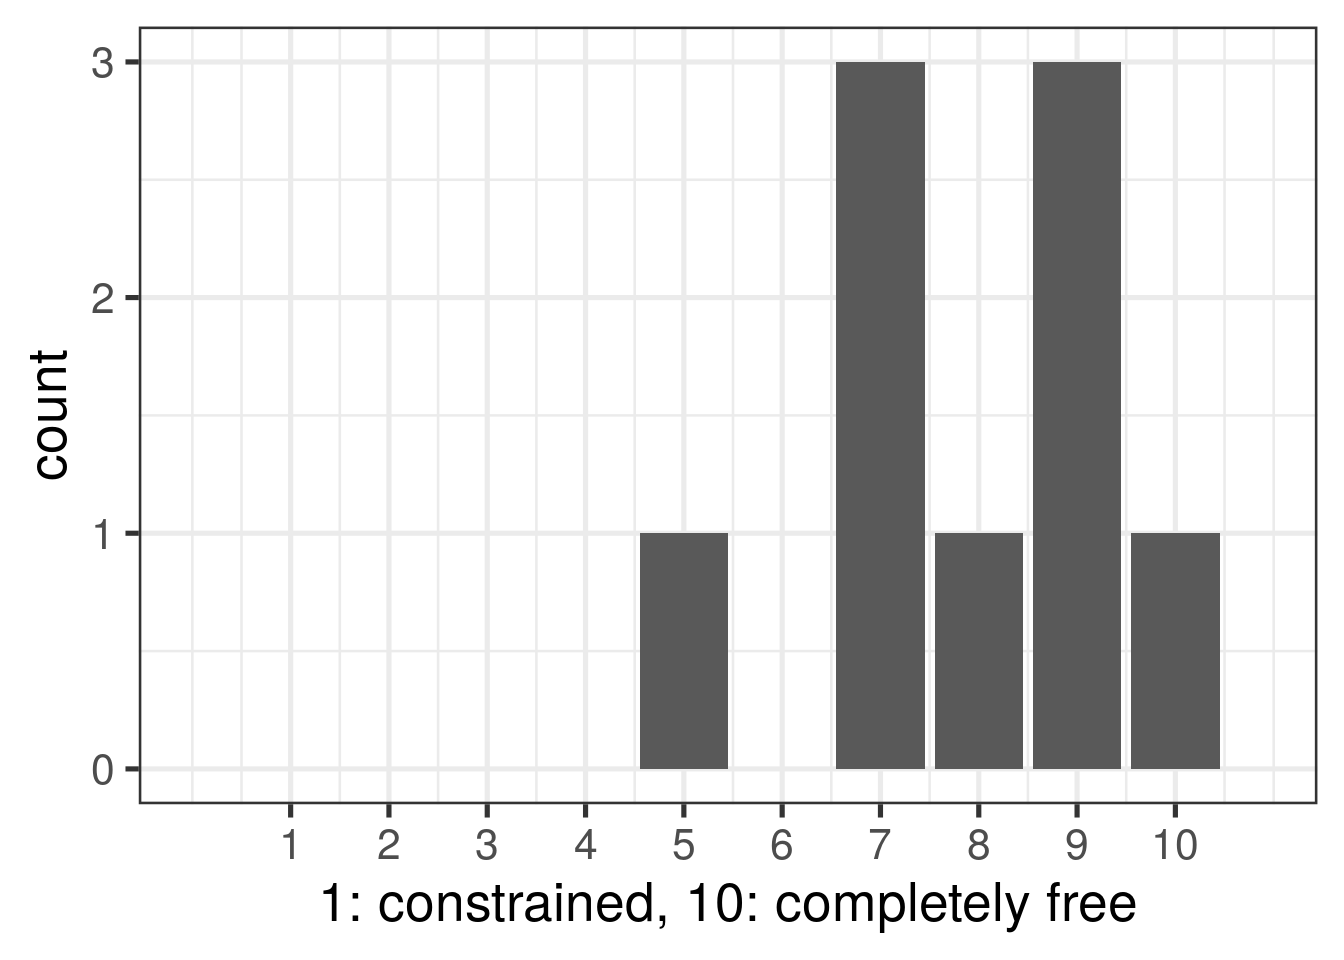
\includegraphics{_main_files/figure-latex/plot_39_2022-04-1.pdf}

\hypertarget{how-collaborative-do-you-think-the-team-is}{%
\section{How collaborative do you think the team is?}\label{how-collaborative-do-you-think-the-team-is}}

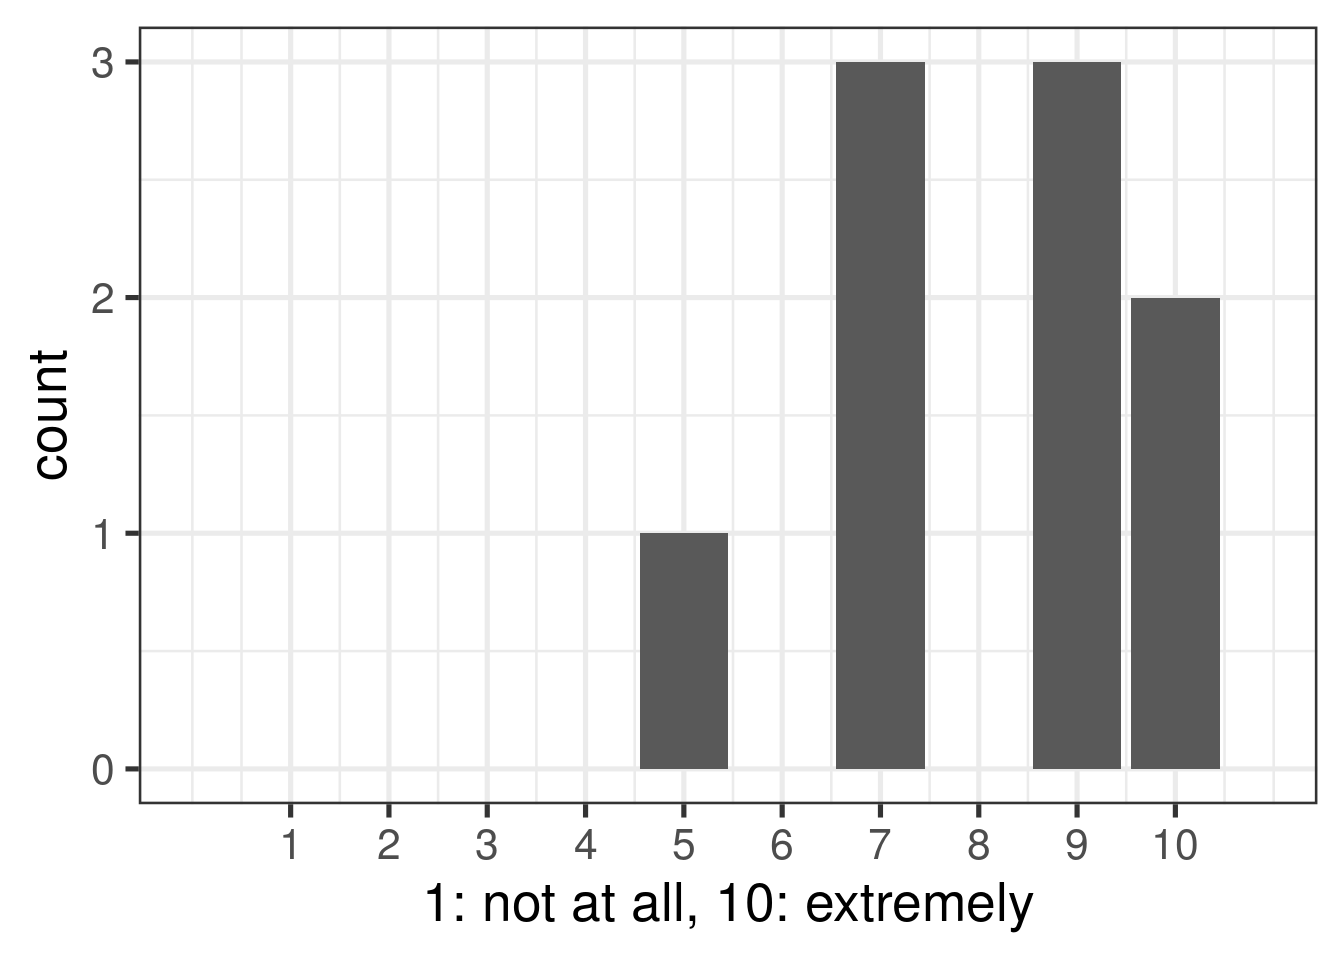
\includegraphics{_main_files/figure-latex/plot_40_2022-04-1.pdf}

\hypertarget{do-you-perceive-that-there-is-any-favoritism-in-the-team-please-elaborate.}{%
\section{Do you perceive that there is any favoritism in the team? Please elaborate.}\label{do-you-perceive-that-there-is-any-favoritism-in-the-team-please-elaborate.}}

\begin{itemize}
\tightlist
\item
  No
\item
  No
\item
  Not really - I would be surprised if there is someone who feels it that way.
\item
  No.
\item
  No
\item
  no
\item
  No
\item
  no
\item
  No, but I am realizing I've been dealt a bad hand with some projects.
\end{itemize}

\hypertarget{are-there-any-issues-with-collaborations-in-the-team-that-are-not-working-please-explain.}{%
\section{Are there any issues with collaborations in the team that are not working? Please explain.}\label{are-there-any-issues-with-collaborations-in-the-team-that-are-not-working-please-explain.}}

\begin{itemize}
\tightlist
\item
  No
\item
  So far, I've seen no issues.
\item
  No
\item
  No
\item
  No
\item
  N/A
\item
  no
\item
  no
\item
  No
\end{itemize}

\hypertarget{are-you-aware-of-the-teams-authorship-policies}{%
\section{Are you aware of the team's authorship policies?}\label{are-you-aware-of-the-teams-authorship-policies}}

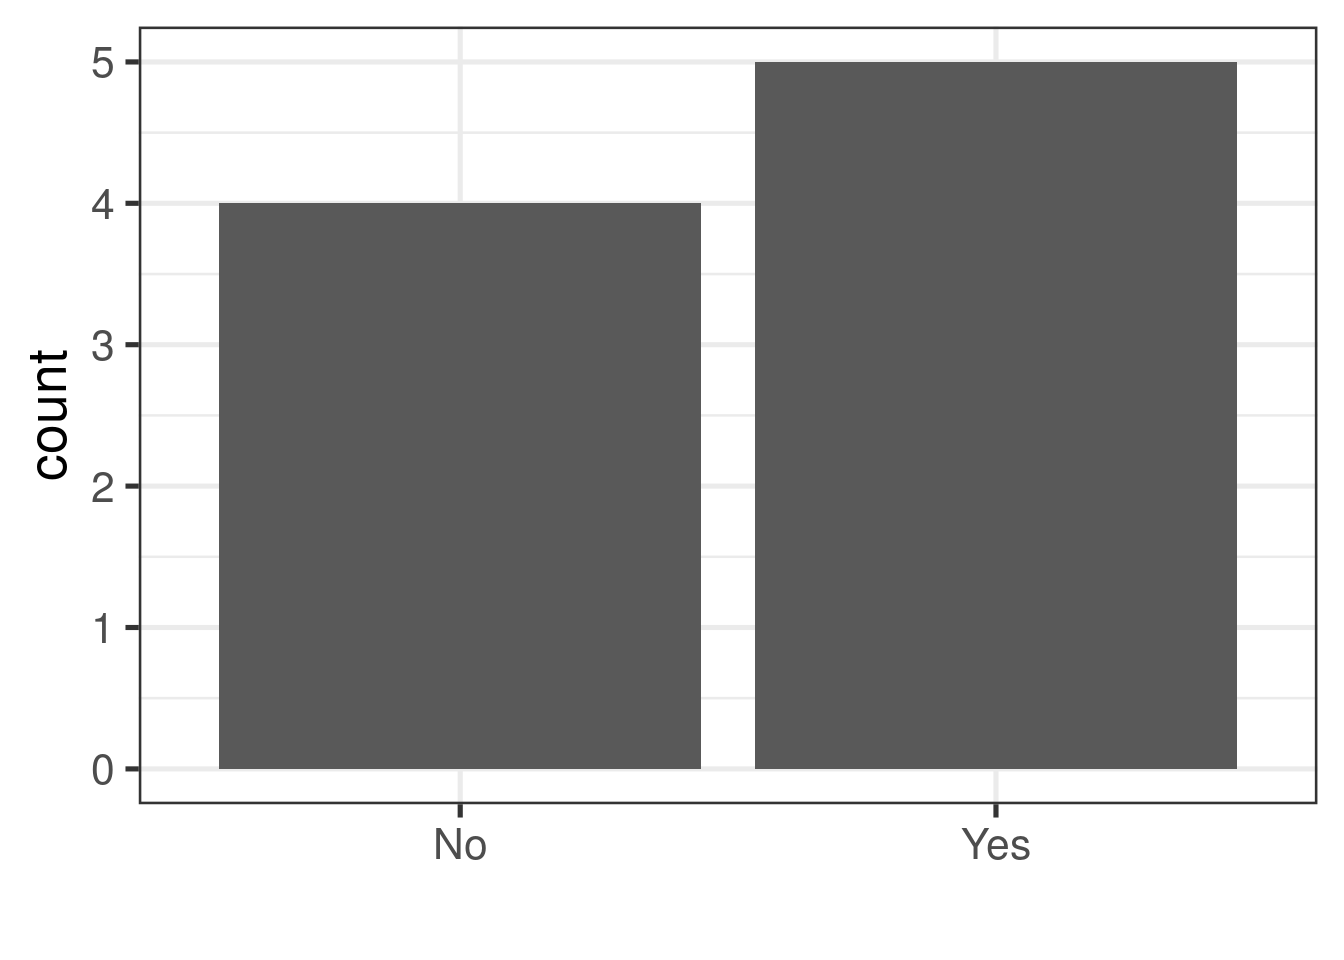
\includegraphics{_main_files/figure-latex/plot_43_2022-04-1.pdf}

\hypertarget{do-have-any-concerns-about-anticipated-authorship-on-papers-describing-your-work-or-collaborations-that-you-are-involved-with}{%
\section{Do have any concerns about anticipated authorship on papers describing your work or collaborations that you are involved with?}\label{do-have-any-concerns-about-anticipated-authorship-on-papers-describing-your-work-or-collaborations-that-you-are-involved-with}}

\begin{itemize}
\tightlist
\item
  no
\item
  No
\item
  No
\item
  Nope
\item
  No
\item
  No
\item
  no
\item
  They're pretty vague
\item
  No
\end{itemize}

\hypertarget{please-rate-whether-you-feel-the-team-provides-you-with-the-tools-and-technologies-you-need}{%
\section{Please rate whether you feel the team provides you with the tools and technologies you need?}\label{please-rate-whether-you-feel-the-team-provides-you-with-the-tools-and-technologies-you-need}}

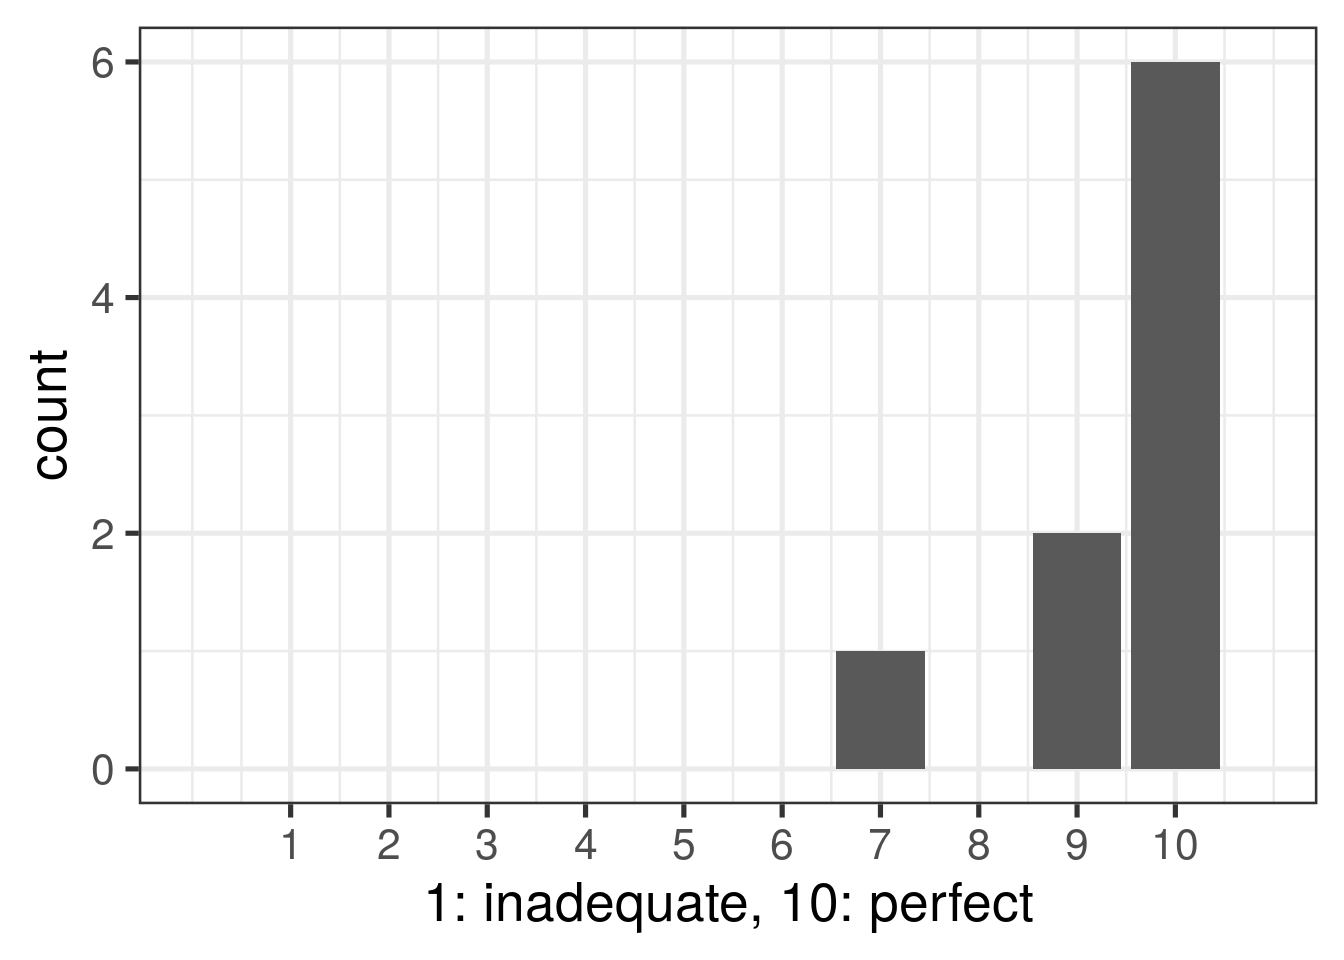
\includegraphics{_main_files/figure-latex/plot_45_2022-04-1.pdf}

\hypertarget{do-you-feel-you-have-received-proper-training-to-perform-the-techniques-required-for-your-work}{%
\section{Do you feel you have received proper training to perform the techniques required for your work?}\label{do-you-feel-you-have-received-proper-training-to-perform-the-techniques-required-for-your-work}}

\begin{itemize}
\tightlist
\item
  Yes for the most part, and I feel that I am given the right resources when needed.
\item
  Yes
\item
  Yes
\item
  Yes
\item
  yes
\item
  I feel like I'm gaining the proper training.
\item
  yes
\item
  N/A - I rely on others for their expertise for now.
\item
  Mostly yes
\end{itemize}

\hypertarget{is-there-further-training-you-would-like-to-receive-to-help-you-accomplish-your-goals}{%
\section{Is there further training you would like to receive to help you accomplish your goals?}\label{is-there-further-training-you-would-like-to-receive-to-help-you-accomplish-your-goals}}

\begin{itemize}
\tightlist
\item
  No
\item
  nothing specific
\item
  I would like more training in statistics
\item
  Recommended free resources for learning/reviewing biostats; maybe a central resources for reviews on technology/methodology, etc. would be really useful
\item
  Python
\item
  Maybe some sort of single cell workshop/bootcamp
\item
  yes
\item
  Yes, I am thinking about it, and I would get back to Leo once I have a better idea about the type of training or what I want to get trained on.
\item
  Maybe, depending on the task.
\end{itemize}

\hypertarget{how-easy-is-it-easy-to-locate-things-in-at-jhpce-github}{%
\section{How easy is it easy to locate things in at JHPCE / GitHub?}\label{how-easy-is-it-easy-to-locate-things-in-at-jhpce-github}}

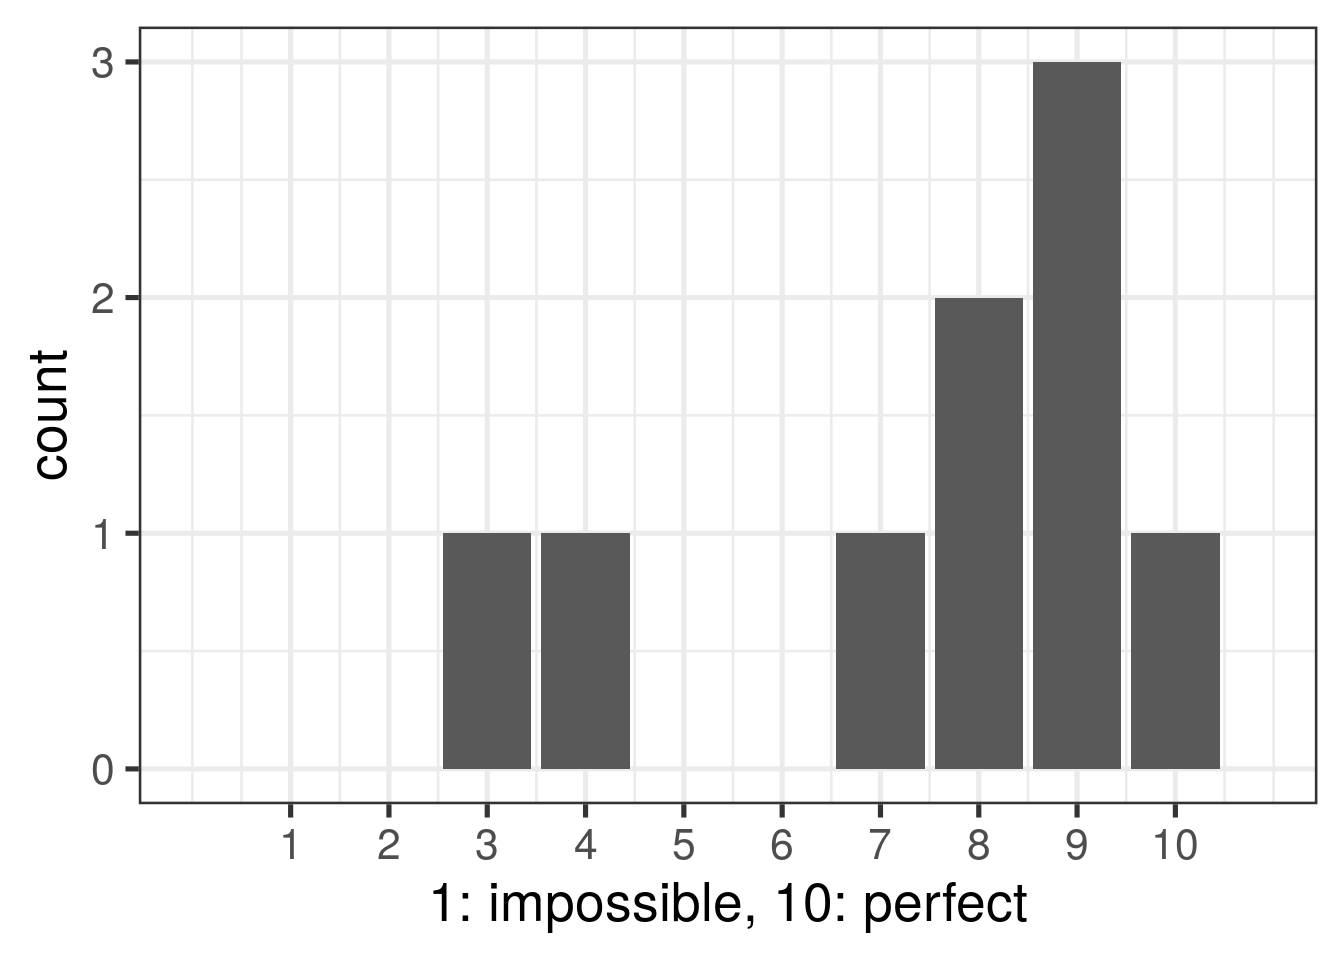
\includegraphics{_main_files/figure-latex/plot_48_2022-04-1.pdf}

\hypertarget{how-often-do-you-encounter-issues-that-could-have-been-averted-if-things-were-better-organized-e.g.-missing-readme-or-github-repository.}{%
\section{How often do you encounter issues that could have been averted if things were better organized? E.g. missing README or GitHub repository.}\label{how-often-do-you-encounter-issues-that-could-have-been-averted-if-things-were-better-organized-e.g.-missing-readme-or-github-repository.}}

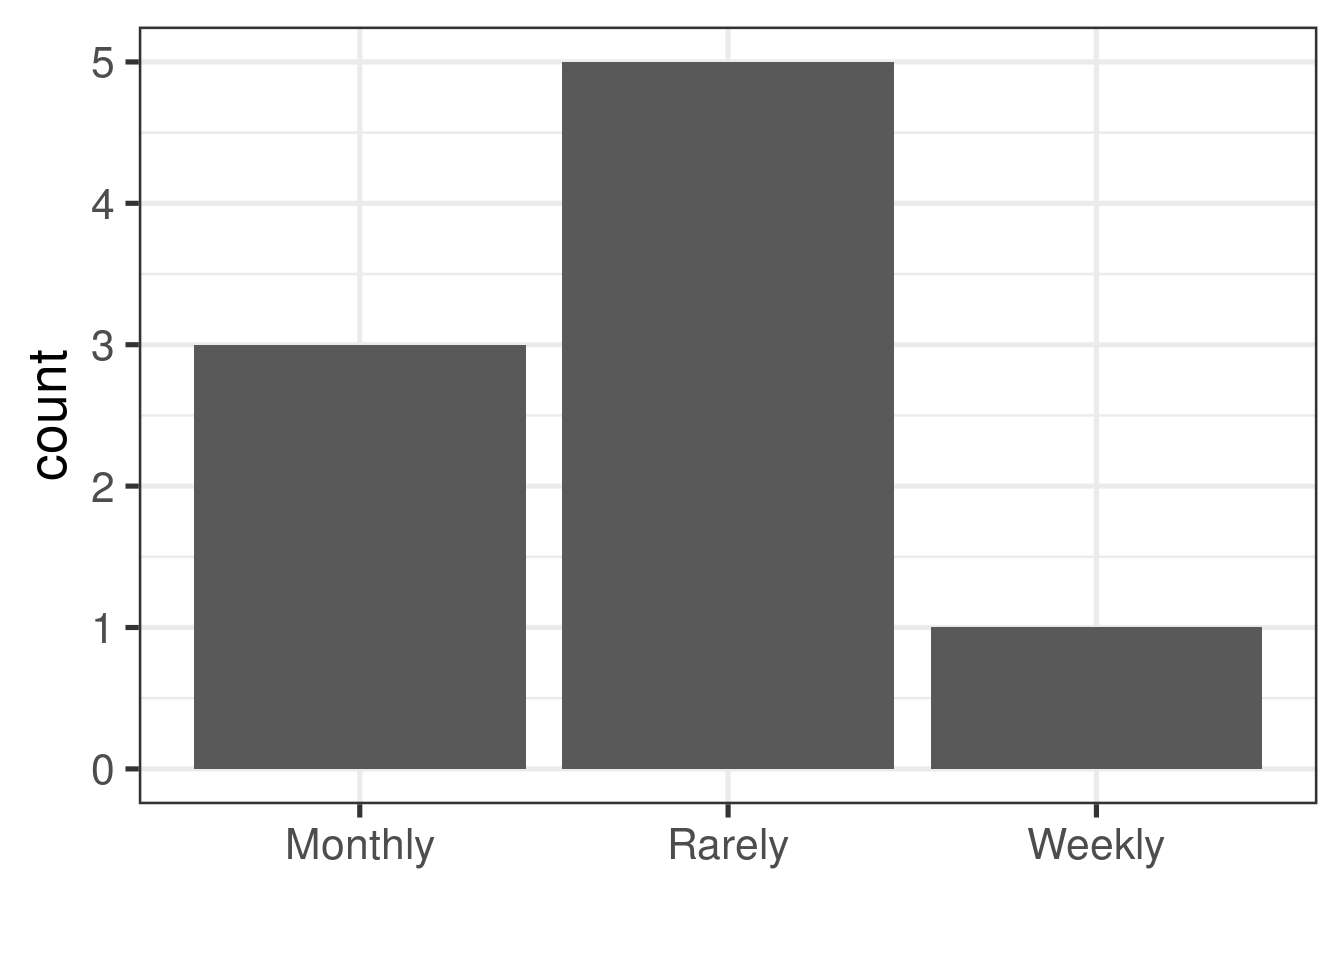
\includegraphics{_main_files/figure-latex/plot_49_2022-04-1.pdf}

\hypertarget{please-tell-me-more-about-the-kinds-of-organizational-issues-you-have-encountered-and-any-suggestions-to-improve-such-issues.}{%
\section{Please tell me more about the kinds of organizational issues you have encountered and any suggestions to improve such issues.}\label{please-tell-me-more-about-the-kinds-of-organizational-issues-you-have-encountered-and-any-suggestions-to-improve-such-issues.}}

\begin{itemize}
\tightlist
\item
  na
\item
  I mostly only work with my repos
\item
  N/A
\item
  Collaborators not using JHPCE/github for their work, and I don't know how to fix this except keep asking \& teaching. But I like the direction we have been headed with JHPCE/project organization, feels like a big improvement from last year!
\item
  N/A
\item
  I have a hard time finding or accessing data that is used in some scripts. If I want to re-run someone's script with their original data, usually I can't find it.
\item
  Code outside of repositories or lacking comments or background context (like a README)
\item
  Haven't faced any yet,
\item
  no issues
\end{itemize}

\hypertarget{what-is-your-opinion-of-the-level-of-technical-support-in-the-team}{%
\section{What is your opinion of the level of technical support in the team?}\label{what-is-your-opinion-of-the-level-of-technical-support-in-the-team}}

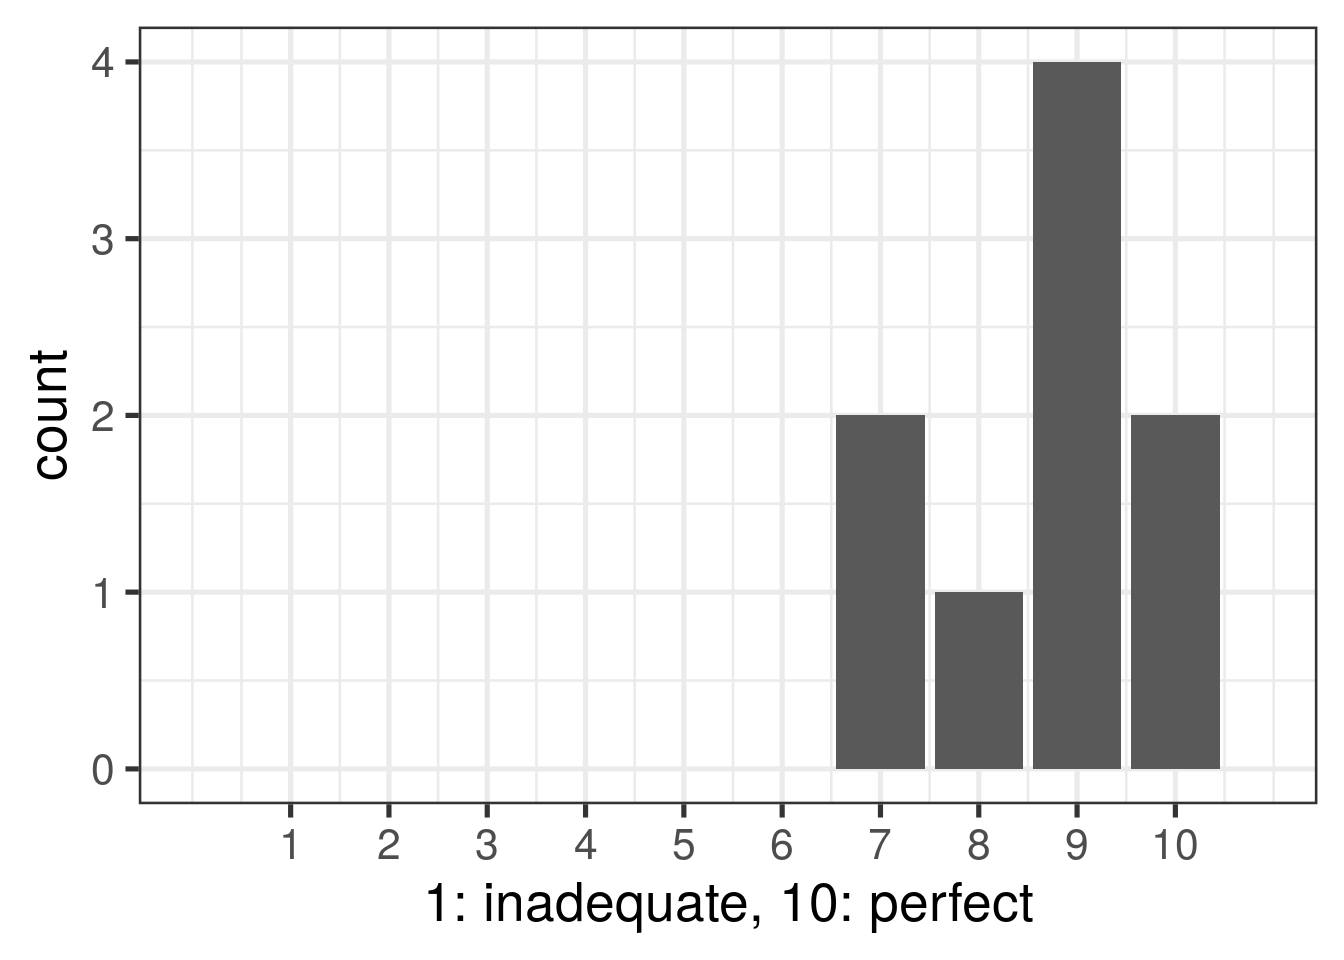
\includegraphics{_main_files/figure-latex/plot_51_2022-04-1.pdf}

\hypertarget{what-is-your-opinion-of-the-level-of-administrative-support-in-the-team}{%
\section{What is your opinion of the level of administrative support in the team?}\label{what-is-your-opinion-of-the-level-of-administrative-support-in-the-team}}

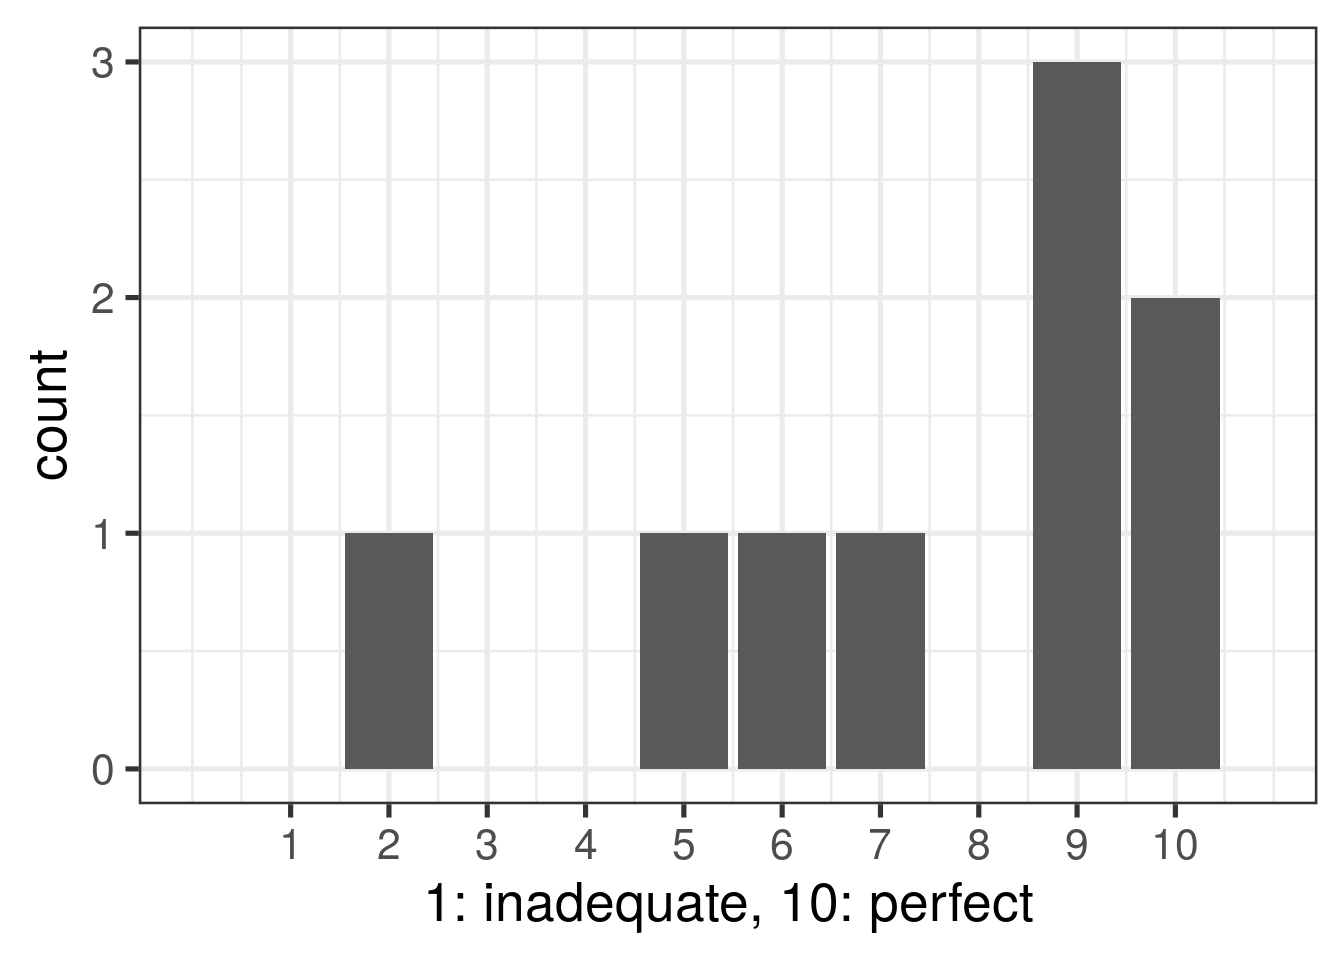
\includegraphics{_main_files/figure-latex/plot_52_2022-04-1.pdf}

\hypertarget{what-is-your-impression-of-the-funding-of-the-team}{%
\section{What is your impression of the funding of the team?}\label{what-is-your-impression-of-the-funding-of-the-team}}

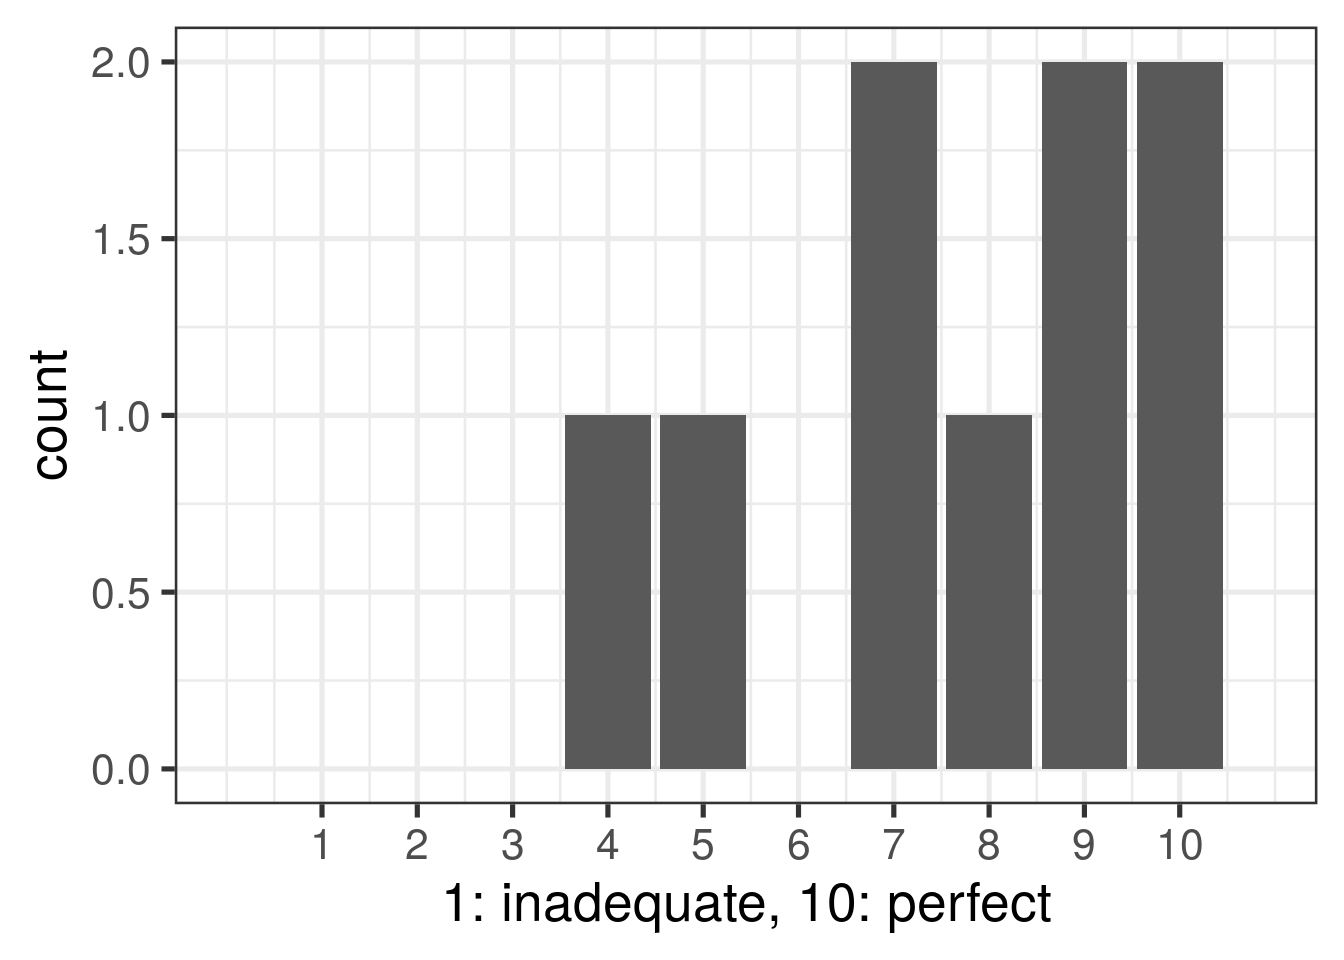
\includegraphics{_main_files/figure-latex/plot_53_2022-04-1.pdf}

\hypertarget{if-we-had-the-funds-to-hire-one-more-full-time-person-what-kind-of-person-should-we-hire-and-what-role-would-they-play-in-the-team}{%
\section{If we had the funds to hire one more full-time person, what kind of person should we hire and what role would they play in the team?}\label{if-we-had-the-funds-to-hire-one-more-full-time-person-what-kind-of-person-should-we-hire-and-what-role-would-they-play-in-the-team}}

\begin{itemize}
\tightlist
\item
  Staff Scientist with engineering heavy abilities
\item
  Someone who is more experienced than us and has good mentorship skills
\item
  A staff scientist still makes sense, who could be another source of knowledge
\item
  N/A
\item
  A staff scientist who could share more of the mentoring roles as Leo
\item
  Staff scientist that could help spread out big projects/spot check work
\item
  I think it could be good to have someone who's dedicated to teaching/lecturing/training.
\item
  a bioinformatics or biostatistics scientist with a strong Computer Science skills to address the more complex computational problems and algorithms
\item
  I don't know
\end{itemize}

\hypertarget{is-there-something-that-you-experienced-in-a-previous-job-that-you-wish-we-also-did-here}{%
\section{Is there something that you experienced in a previous job that you wish we also did here?}\label{is-there-something-that-you-experienced-in-a-previous-job-that-you-wish-we-also-did-here}}

\begin{itemize}
\tightlist
\item
  Frequently we updated on what progress others were making.
\item
  NA
\item
  no
\item
  No
\item
  N/A
\item
  Culture surveys for the broader institute
\item
  This place is a way better than my previous workplace almost in every aspect - this is not a lie.
\item
  No
\item
  NA
\end{itemize}

\hypertarget{are-there-any-concerns-or-other-areas-of-the-team-you-believe-could-be-improved-that-have-not-been-addressed-in-previous-questions-please-list-any-other-areas-you-think-could-be-improved-or-should-be-addressed.}{%
\section{Are there any concerns or other areas of the team you believe could be improved that have not been addressed in previous questions? Please list any other areas you think could be improved or should be addressed.}\label{are-there-any-concerns-or-other-areas-of-the-team-you-believe-could-be-improved-that-have-not-been-addressed-in-previous-questions-please-list-any-other-areas-you-think-could-be-improved-or-should-be-addressed.}}

\begin{itemize}
\tightlist
\item
  no
\item
  N/A
\item
  The gap in pay due to inflation and a robust biotech market is such that we will continue to lose colleagues and have vacancies if we cannot figure out compensation.
\item
  No.~I think Leo is a great mentor
\item
  This is pretty thorough!
\item
  N/A
\item
  Nope.
\item
  no
\item
  No
\end{itemize}

\hypertarget{finally-did-you-find-this-survey-useful-if-yes-how-often-should-the-survey-be-conducted}{%
\section{Finally, did you find this survey useful? If yes, how often should the survey be conducted?}\label{finally-did-you-find-this-survey-useful-if-yes-how-often-should-the-survey-be-conducted}}

\begin{itemize}
\tightlist
\item
  Yes s, annually
\item
  Yes.
\item
  Yes. Yearly.
\item
  Yes, somewhat useful. Yearly seems adequate.
\item
  Yes, it felt more useful the first time we did it. Its pretty long and since there were no drastic changes from last year so it felt a bit redundant at times. Yearly is probably the correct interval but maybe extract some questions sections out for their own survey, for instance the ``Mentoring'' questions may be best to ask after we have done performance reviews/career meetings for the year so that experience is fresh. I think if it was more concise I could be more sure I gave high quality answers for each point.
\item
  Yes, annually is ok
\item
  Yes, yearly sounds perfect
\item
  Yes! Maybe twice a year
\item
  It is useful. As a collaborator, I found myself limited or found it somewhat hard to do the survey because I think many of the questions were specific to Leo's team and culture, which I might not be familiar with. But, I would agree that doing this often will be helpful as a sanity check for the team environment.
\end{itemize}

\hypertarget{survey-2021-03}{%
\chapter{Survey 2021-03}\label{survey-2021-03}}

\hypertarget{what-3-words-would-you-use-to-describe-our-team-culture-1}{%
\section{What 3 words would you use to describe our team culture?}\label{what-3-words-would-you-use-to-describe-our-team-culture-1}}

\begin{itemize}
\tightlist
\item
  independent, relaxed, supportive
\item
  organized/helpful/friendly
\item
  supportive, dedicated, curious
\item
  collaborative, supportive, productive
\item
  Helpful, safe, encouraging
\item
  Independent, creative, supportive
\end{itemize}

\hypertarget{what-do-you-like-most-about-working-here-1}{%
\section{What do you like most about working here?}\label{what-do-you-like-most-about-working-here-1}}

\begin{itemize}
\tightlist
\item
  Getting to learn so many new things in a not super stressful way
\item
  Lots of room to grow, no expectation that you know everything, and very supportive of people learning new things
\item
  my colleagues are great
\item
  Learning loads of things that are really helpful for my scientific career in a team where everyone is happy to help, and where the PI is giving me feedback and pushing me to grow. Also I like that the human part is not lost.
\item
  Support for learning and career development at every stage
\item
  There's a huge amount to learn, and opportunity to improve many skills
\end{itemize}

\hypertarget{what-do-you-like-least-about-working-here-1}{%
\section{What do you like least about working here?}\label{what-do-you-like-least-about-working-here-1}}

\begin{itemize}
\tightlist
\item
  I don't think there is something I dislike
\item
  NA
\item
  Too many slack channels
\item
  pay and career growth are questionable
\item
  Can sometimes fell a bit isolated, but thats probably more an issue with remote work in general
\item
  There is sometimes not enough context or explanation given for the goals of a project, which can make it hard to jump in.
\end{itemize}

\hypertarget{how-happy-are-you-in-the-team-1}{%
\section{How happy are you in the team?}\label{how-happy-are-you-in-the-team-1}}

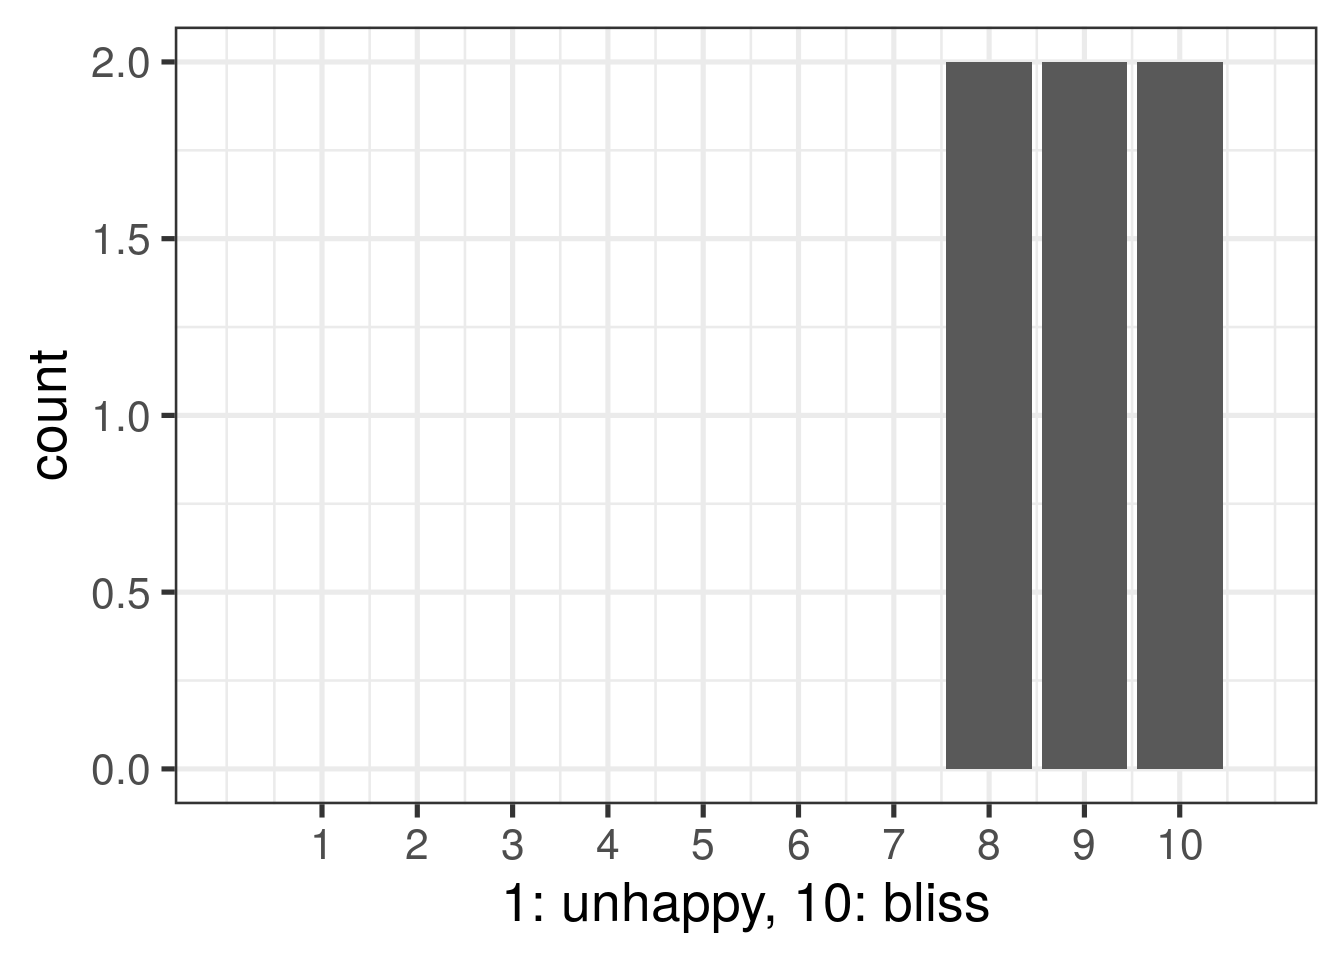
\includegraphics{_main_files/figure-latex/plot_5_2021-03-1.pdf}

\hypertarget{is-there-something-that-could-be-provided-to-make-you-happier-1}{%
\section{Is there something that could be provided to make you happier?}\label{is-there-something-that-could-be-provided-to-make-you-happier-1}}

\begin{itemize}
\tightlist
\item
  Excited to get back in the lab and work more closely with others
\item
  upward career path.
\item
  Weighted blankets
\item
  No
\item
  I like working on projects with one other person
\item
  No.
\end{itemize}

\hypertarget{what-is-your-impression-of-social-life-in-the-team-too-social-not-enough-or-just-right-if-you-want-to-improve-the-social-life-in-the-lab-what-are-your-suggestions-for-achieving-this-1}{%
\section{What is your impression of social life in the team? Too social, not enough, or just right? If you want to improve the social life in the lab, what are your suggestions for achieving this?}\label{what-is-your-impression-of-social-life-in-the-team-too-social-not-enough-or-just-right-if-you-want-to-improve-the-social-life-in-the-lab-what-are-your-suggestions-for-achieving-this-1}}

\begin{itemize}
\tightlist
\item
  Social life is right
\item
  once the pandemic is closer i think the team will get to know each other better.
\item
  It feels not quite social enough, but this probably mostly has to do with inherent COVID restrictions which can't be easily avoided. I'm not sure the best way to improve.
\item
  Hard to answer this question given that we've been WFH for over a year - I think we are the right amount of social
\item
  I think we could be a bit more social, but it's difficult right now during the pandemic
\item
  I think we are doing what we can with the extenuating circumstances. I am glad we are getting back to doing happy hours now the weather is nice.
\end{itemize}

\hypertarget{how-comfortable-do-you-feel-sharing-personal-concerns-housing-financial-family-physical-or-mental-health-with-me-1}{%
\section{How comfortable do you feel sharing personal concerns (housing, financial, family, physical or mental health) with me?}\label{how-comfortable-do-you-feel-sharing-personal-concerns-housing-financial-family-physical-or-mental-health-with-me-1}}

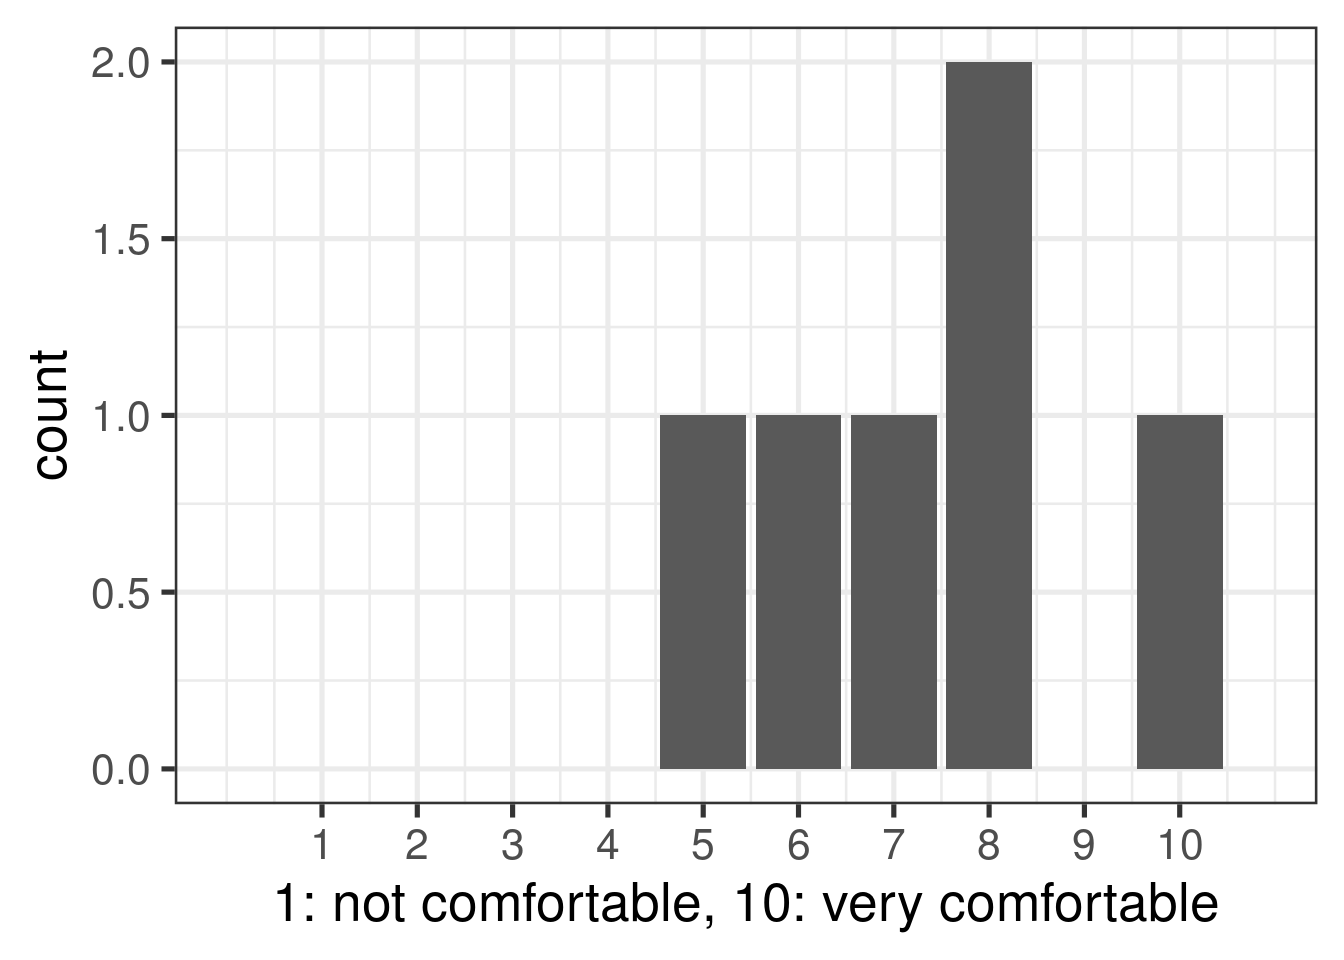
\includegraphics{_main_files/figure-latex/plot_8_2021-03-1.pdf}

\hypertarget{do-you-feel-explicit-or-implicit-pressure-to-work-more-hours-than-you-feel-is-healthy-1}{%
\section{Do you feel explicit or implicit pressure to work more hours than you feel is healthy?}\label{do-you-feel-explicit-or-implicit-pressure-to-work-more-hours-than-you-feel-is-healthy-1}}

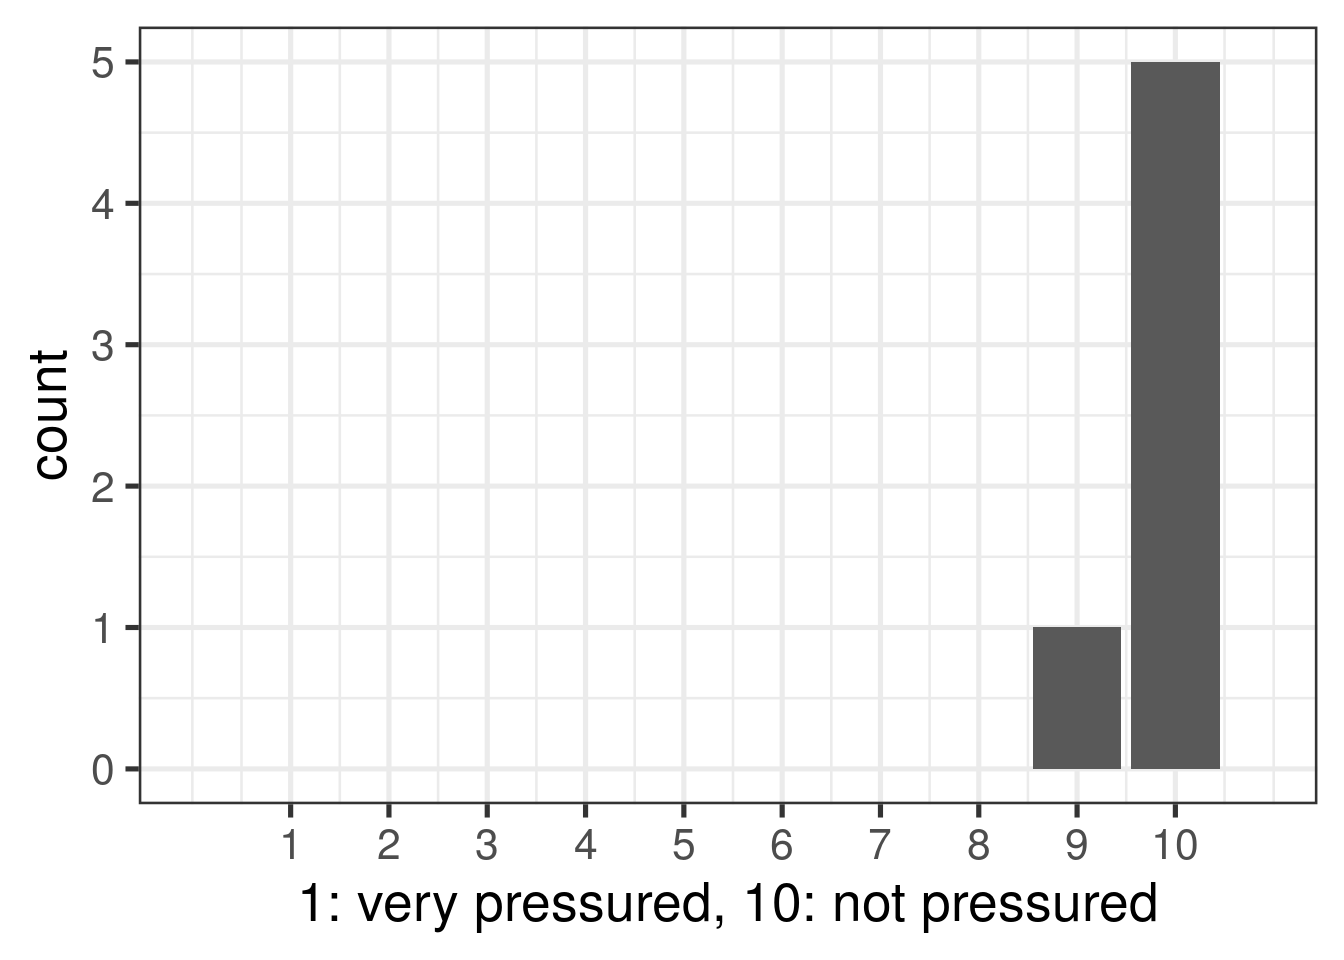
\includegraphics{_main_files/figure-latex/plot_9_2021-03-1.pdf}

\hypertarget{do-you-feel-explicit-or-implicit-pressure-to-avoid-taking-vacations-1}{%
\section{Do you feel explicit or implicit pressure to avoid taking vacations?}\label{do-you-feel-explicit-or-implicit-pressure-to-avoid-taking-vacations-1}}

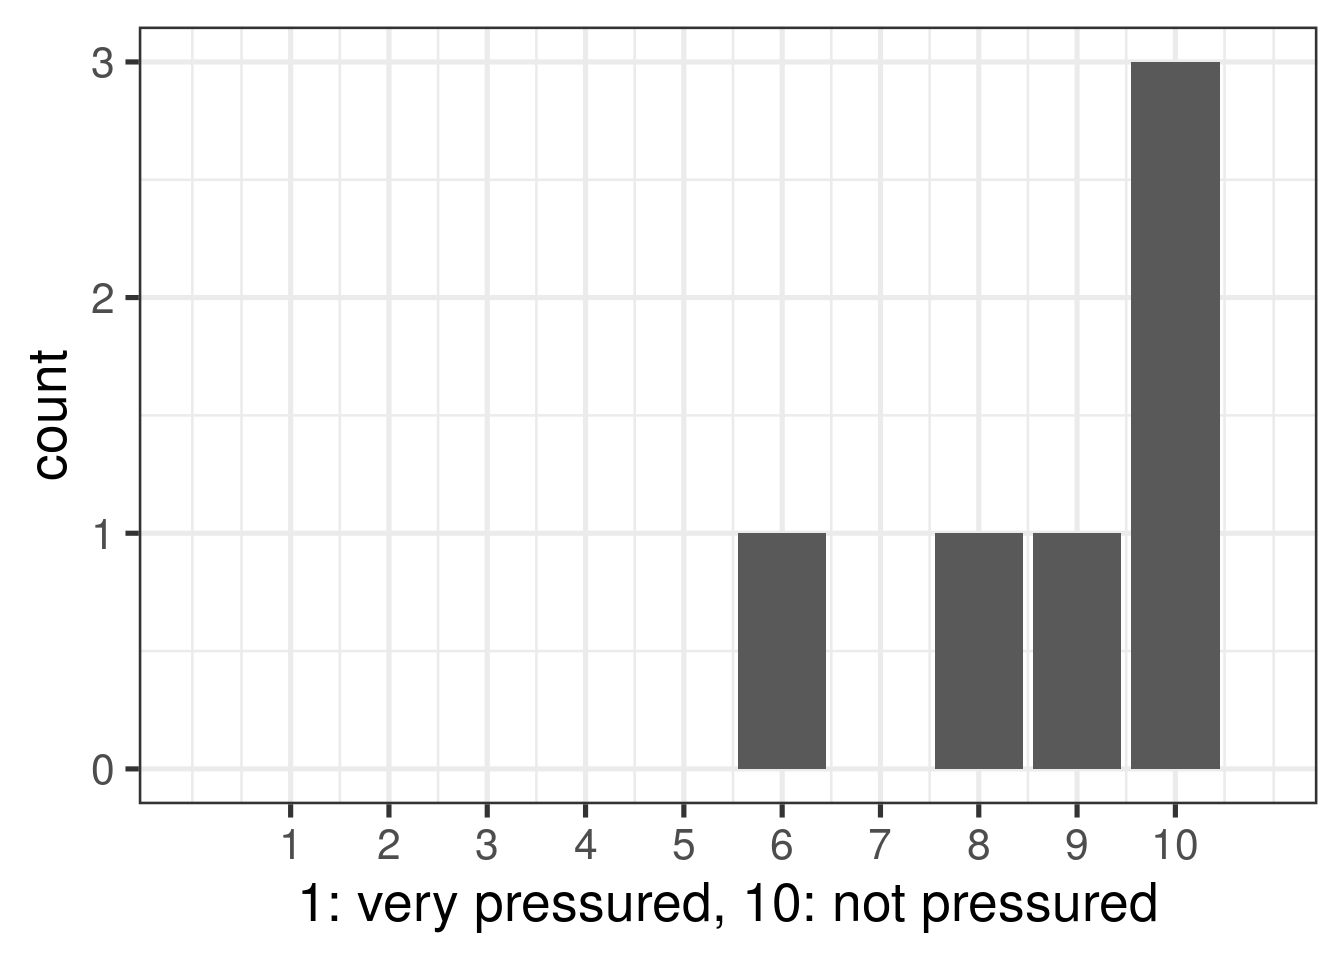
\includegraphics{_main_files/figure-latex/plot_10_2021-03-1.pdf}

\hypertarget{have-you-experienced-or-witnessed-a-hostile-work-environment-in-the-team-bullying-gender-harassment-sexual-harassment-1}{%
\section{Have you experienced or witnessed a hostile work environment in the team? (bullying, gender harassment, sexual harassment)}\label{have-you-experienced-or-witnessed-a-hostile-work-environment-in-the-team-bullying-gender-harassment-sexual-harassment-1}}

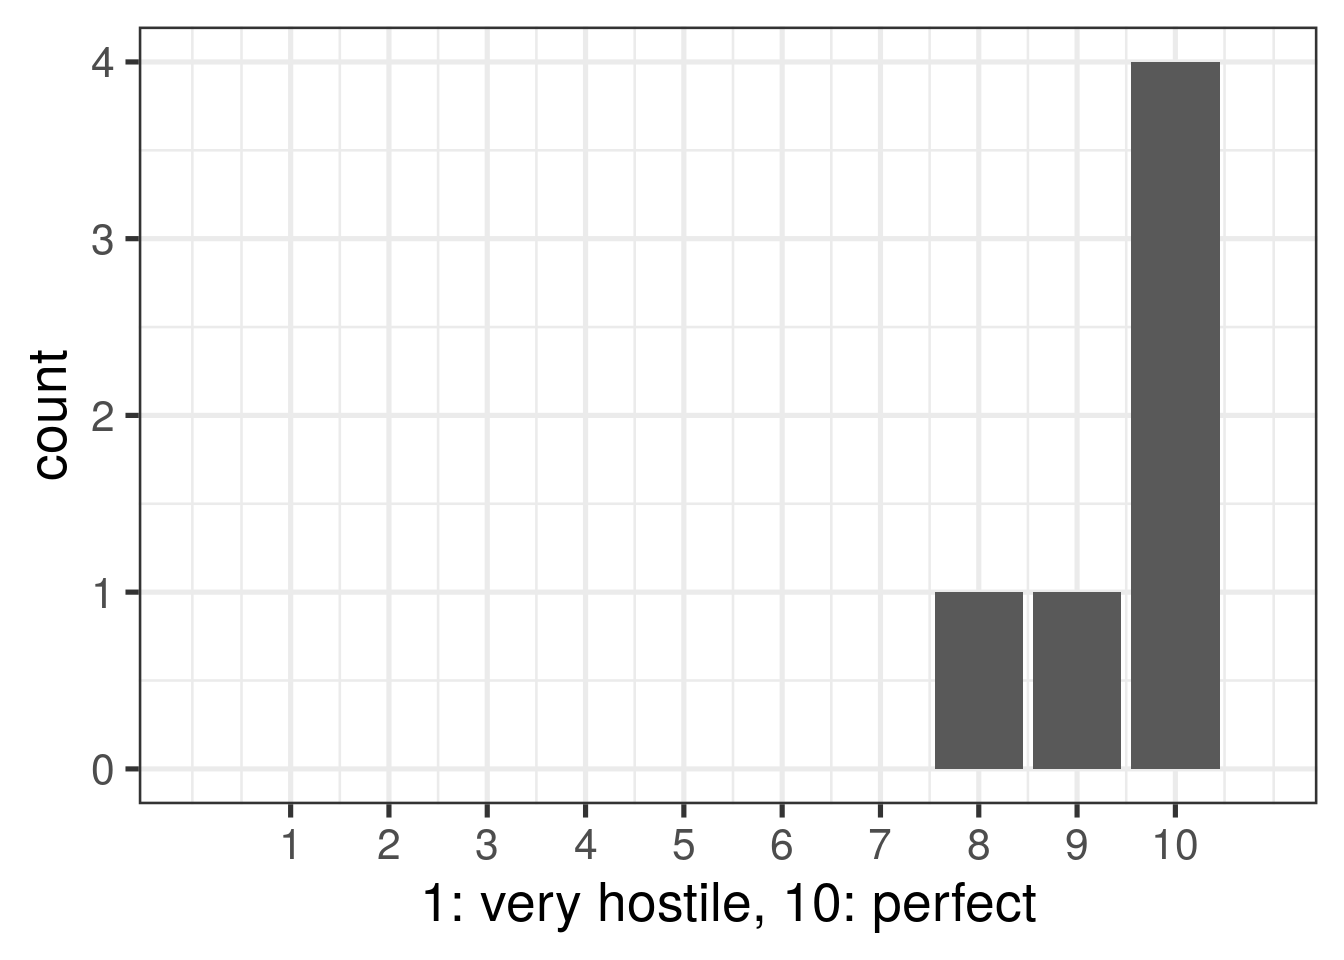
\includegraphics{_main_files/figure-latex/plot_11_2021-03-1.pdf}

\hypertarget{how-well-does-the-team-communicate-as-a-whole-1}{%
\section{How well does the team communicate as a whole?}\label{how-well-does-the-team-communicate-as-a-whole-1}}

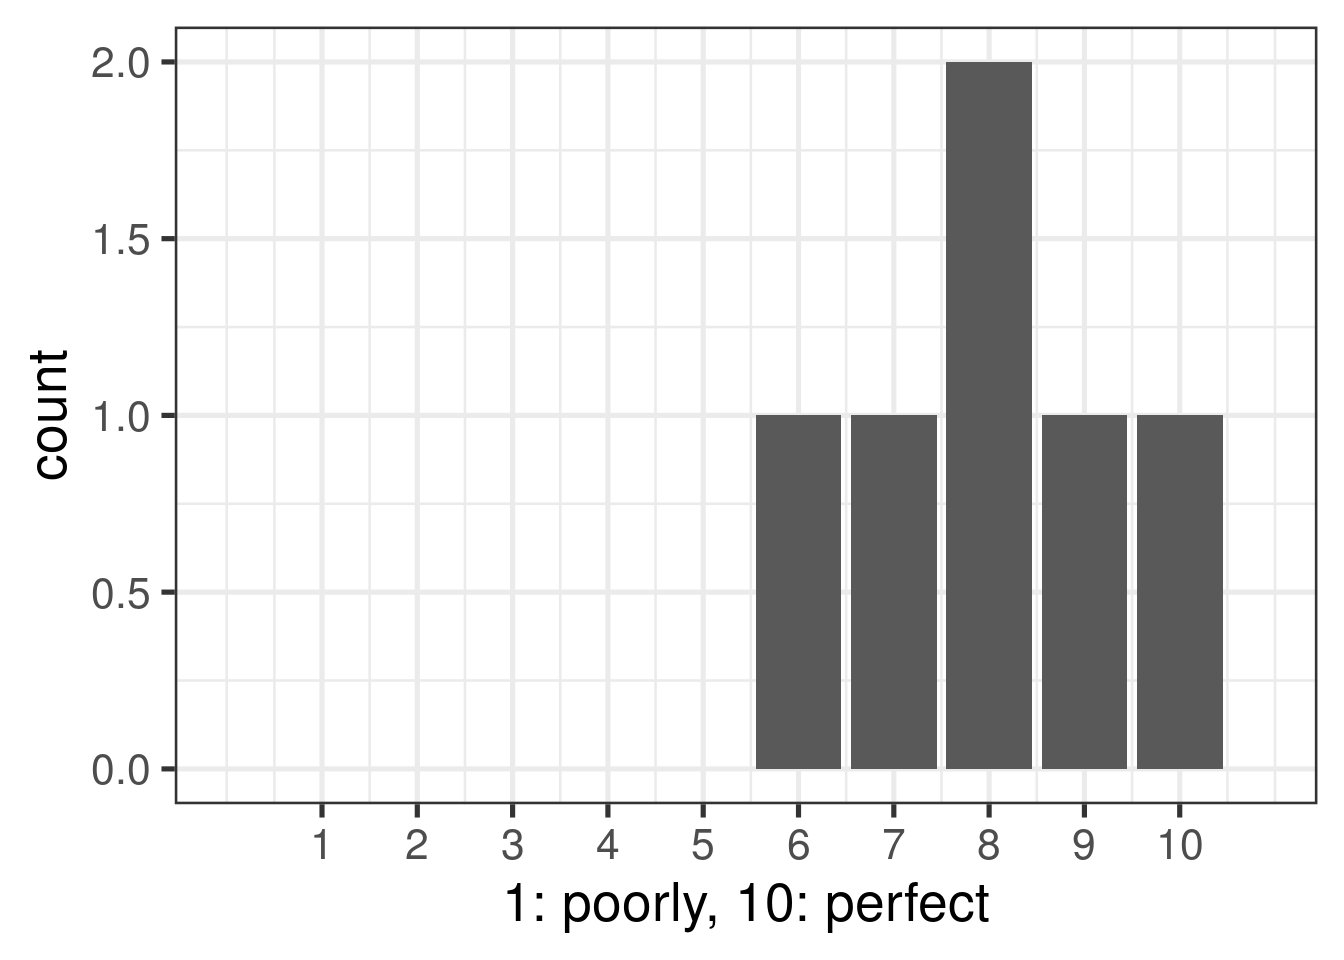
\includegraphics{_main_files/figure-latex/plot_12_2021-03-1.pdf}

\hypertarget{what-are-some-ways-that-we-could-improve-communication-in-the-team-1}{%
\section{What are some ways that we could improve communication in the team?}\label{what-are-some-ways-that-we-could-improve-communication-in-the-team-1}}

\begin{itemize}
\tightlist
\item
  I feel like whatever answer I would give to this question is less relevant now that Lieber is opening back up
\item
  I think that we communicate very well.
\item
  We need to encourage more collaboration to develop less experienced members as well as encourage people to ask for help faster.
\item
  On personal projects, it's sometimes hard to get as much external feedback as would be ideal. Assigning multiple people to a particular project can improve internal communication and reduce the need for frequent feedback from you.
\item
  I think it is ok and slack is a perfect platform to do it.
\item
  I liked discussing the ``nuts and bolts'' of our cluster usage/needs. Maybe we can focus some of our lab discussions on the tech/code side in addition to the science side. Also we never really put together the code review sessions and I feel like that would be a useful tool. Some times I am unsure which meetings I am expected to attend.
\end{itemize}

\hypertarget{do-you-feel-that-lab-rulespolicies-are-clear-are-there-unspoken-rules-or-policies-that-you-feel-should-be-more-clearly-communicated-1}{%
\section{Do you feel that lab rules/policies are clear? Are there unspoken rules or policies that you feel should be more clearly communicated?}\label{do-you-feel-that-lab-rulespolicies-are-clear-are-there-unspoken-rules-or-policies-that-you-feel-should-be-more-clearly-communicated-1}}

\begin{itemize}
\tightlist
\item
  I feel pretty good about policies
\item
  Rules are clear.
\item
  Lab rules are clear to me
\item
  I guess most rules are unspoken. I don't think we have a behavioral issue but any specific policies could be put in writing.
\item
  if I had to give one, I would say baseline expectations across all projects
\item
  Rules are clear.
\end{itemize}

\hypertarget{are-there-policies-you-feel-should-be-explicitly-written-if-so-please-explain-which-ones.-1}{%
\section{Are there policies you feel should be explicitly written? If so, please explain which ones.}\label{are-there-policies-you-feel-should-be-explicitly-written-if-so-please-explain-which-ones.-1}}

\begin{itemize}
\tightlist
\item
  NA
\item
  No
\item
  No.
\item
  No
\item
  No
\item
  Guidelines for data privacy, what should we be careful to keep secure?
\end{itemize}

\hypertarget{do-you-feel-that-the-same-rules-apply-to-everyone-in-team-if-not-please-explain.-1}{%
\section{Do you feel that the same rules apply to everyone in team? If not, please explain.}\label{do-you-feel-that-the-same-rules-apply-to-everyone-in-team-if-not-please-explain.-1}}

\begin{itemize}
\item
  Yes
\item
  Yes
\item
  Yes.
\item
  Yes
\item
  yes
\item
  \begin{itemize}
  \tightlist
  \item
  \end{itemize}
\end{itemize}

\hypertarget{do-you-feel-empowered-to-make-suggestions-to-me-to-improve-the-team-culture-organization-1}{%
\section{Do you feel empowered to make suggestions to me to improve the team culture/ organization?}\label{do-you-feel-empowered-to-make-suggestions-to-me-to-improve-the-team-culture-organization-1}}

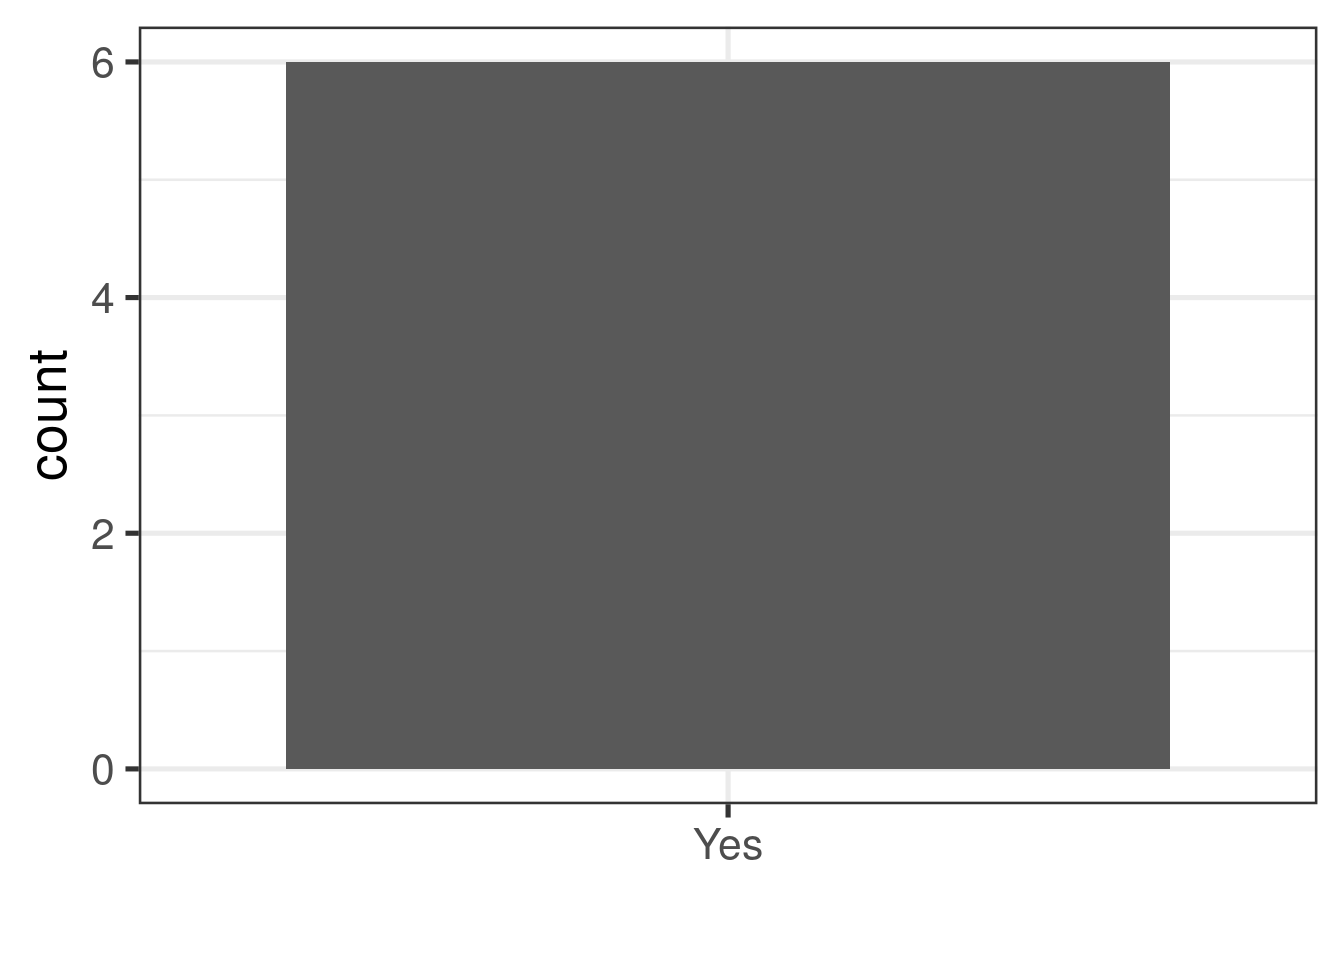
\includegraphics{_main_files/figure-latex/plot_17_2021-03-1.pdf}

\hypertarget{do-you-feel-empowered-to-make-suggestions-to-your-colleagues-to-improve-the-team-culture-organization-1}{%
\section{Do you feel empowered to make suggestions to your colleagues to improve the team culture/ organization?}\label{do-you-feel-empowered-to-make-suggestions-to-your-colleagues-to-improve-the-team-culture-organization-1}}

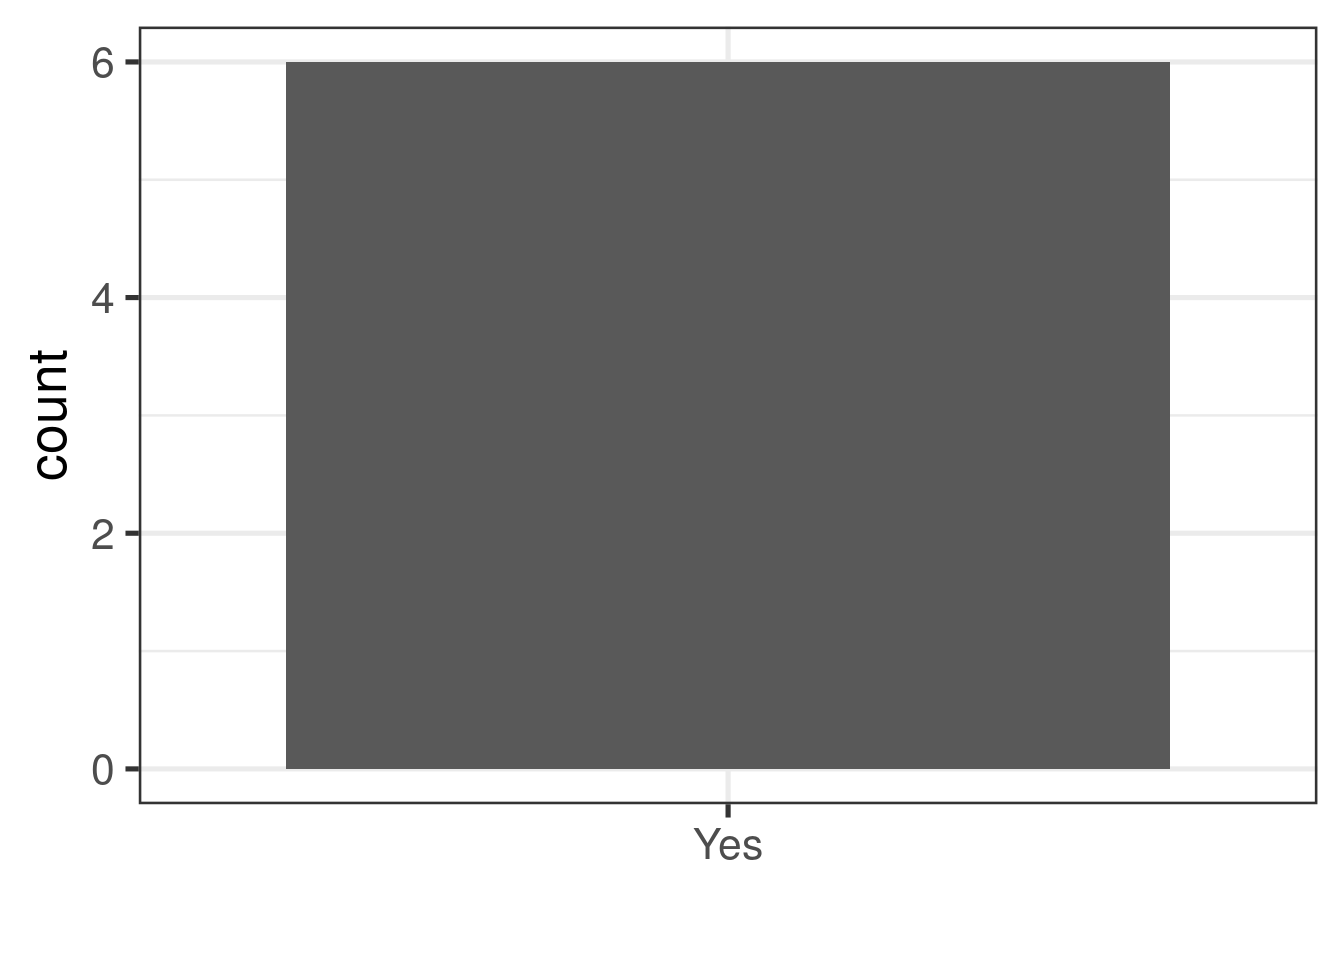
\includegraphics{_main_files/figure-latex/plot_18_2021-03-1.pdf}

\hypertarget{if-you-do-not-feel-empowered-to-make-suggestions-to-your-colleagues-in-the-team-or-to-me-to-improve-the-team-culture-organization-please-tell-me-more-about-this.-1}{%
\section{If you do not feel empowered to make suggestions to your colleagues in the team or to me to improve the team culture/ organization, please tell me more about this.}\label{if-you-do-not-feel-empowered-to-make-suggestions-to-your-colleagues-in-the-team-or-to-me-to-improve-the-team-culture-organization-please-tell-me-more-about-this.-1}}

\begin{itemize}
\item
  \begin{itemize}
  \tightlist
  \item
  \end{itemize}
\item
  NA
\item
  N/A
\item
  N/A
\item
  NA
\item
  NA
\end{itemize}

\hypertarget{do-you-feel-you-have-enough-feedback-on-your-project-1}{%
\section{Do you feel you have enough feedback on your project?}\label{do-you-feel-you-have-enough-feedback-on-your-project-1}}

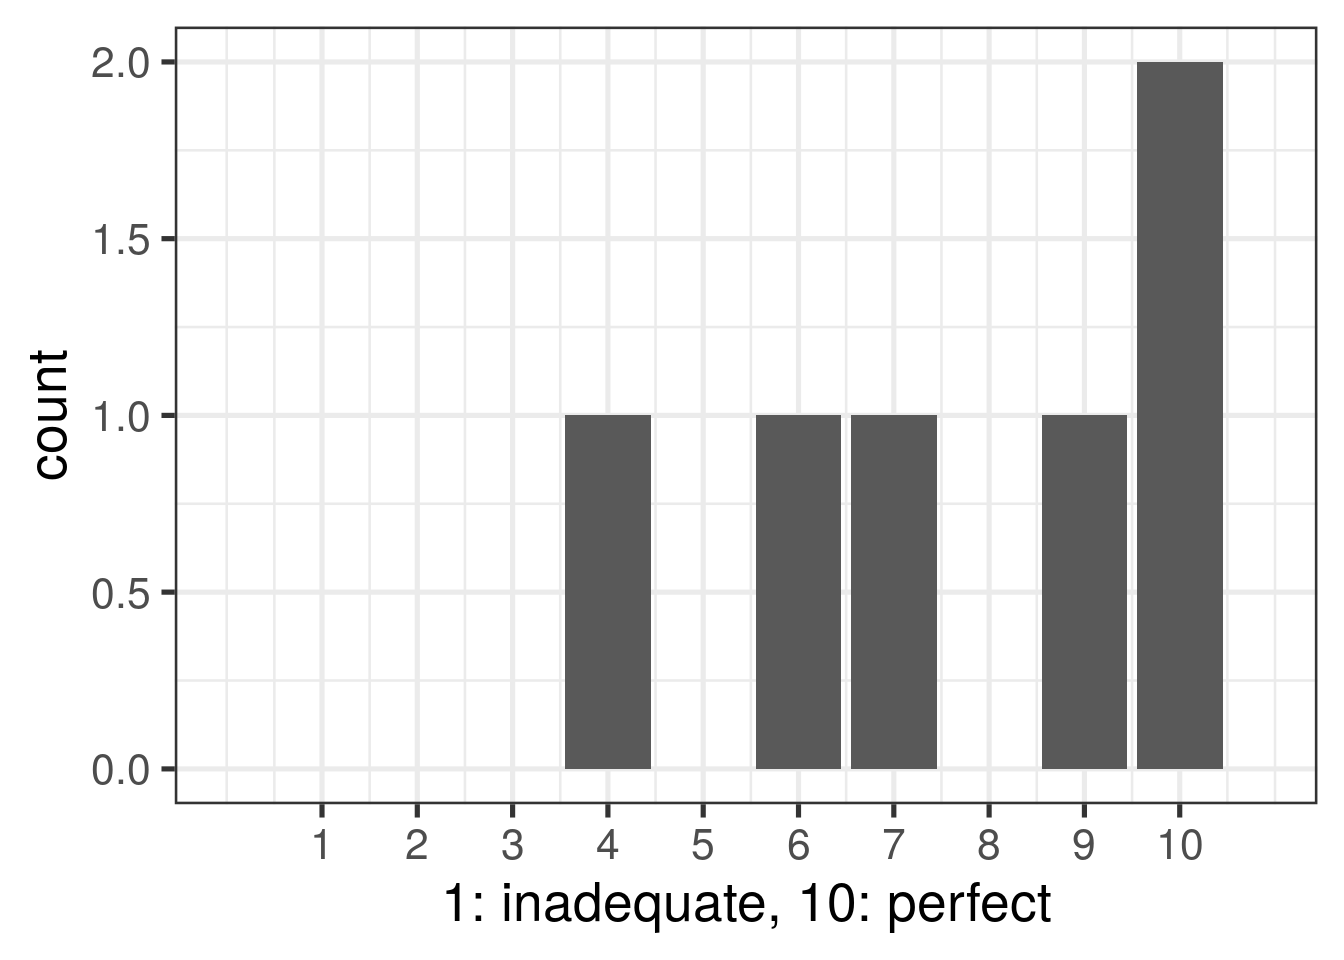
\includegraphics{_main_files/figure-latex/plot_20_2021-03-1.pdf}

\hypertarget{do-you-feel-you-have-enough-time-to-meet-with-me-1}{%
\section{Do you feel you have enough time to meet with me?}\label{do-you-feel-you-have-enough-time-to-meet-with-me-1}}

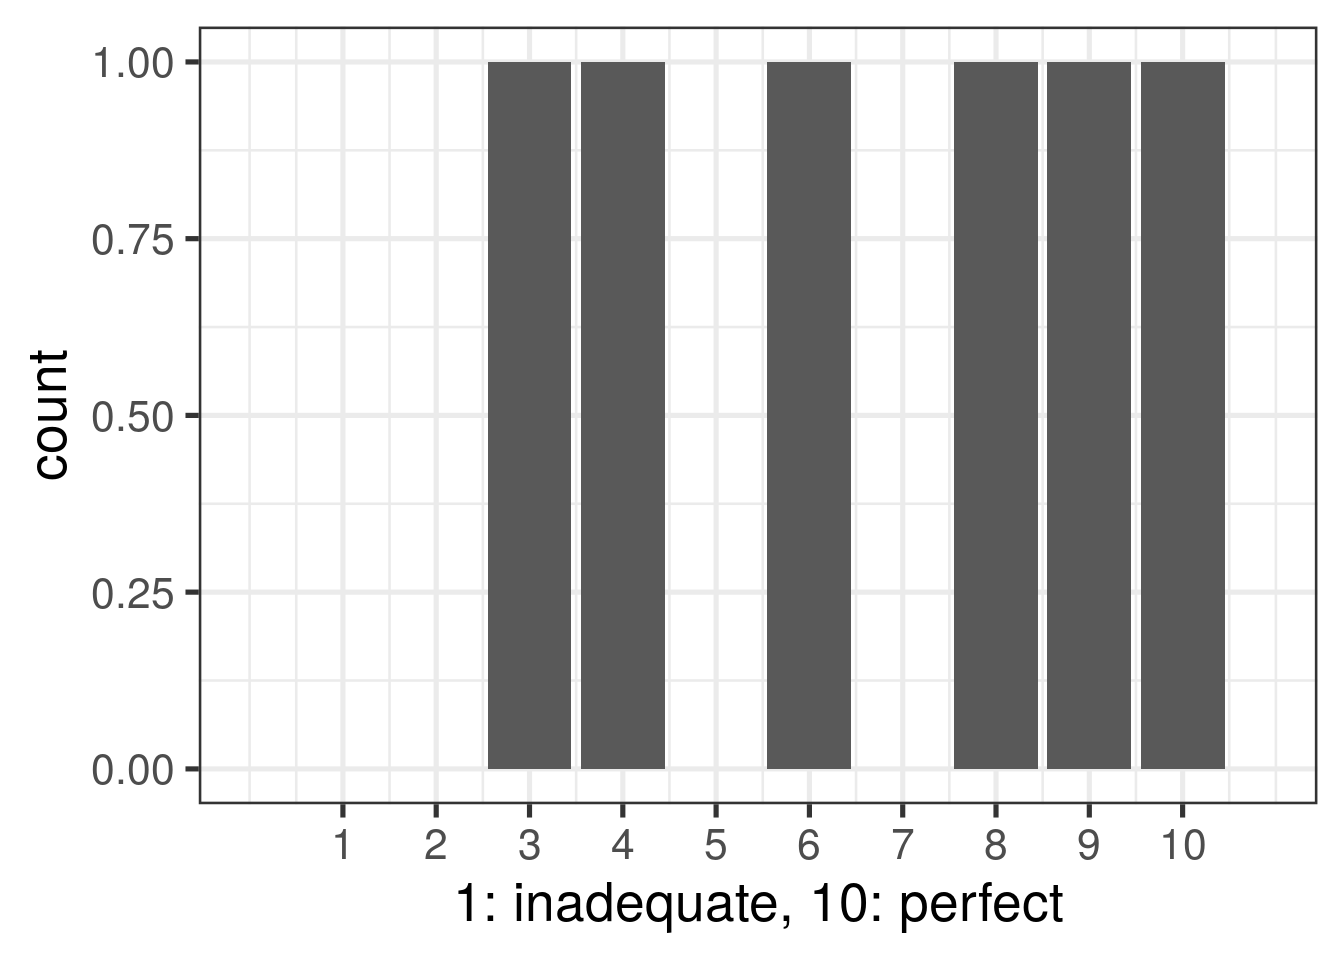
\includegraphics{_main_files/figure-latex/plot_21_2021-03-1.pdf}

\hypertarget{how-useful-do-you-find-one-on-one-meetings-with-me-1}{%
\section{How useful do you find one-on-one meetings with me?}\label{how-useful-do-you-find-one-on-one-meetings-with-me-1}}

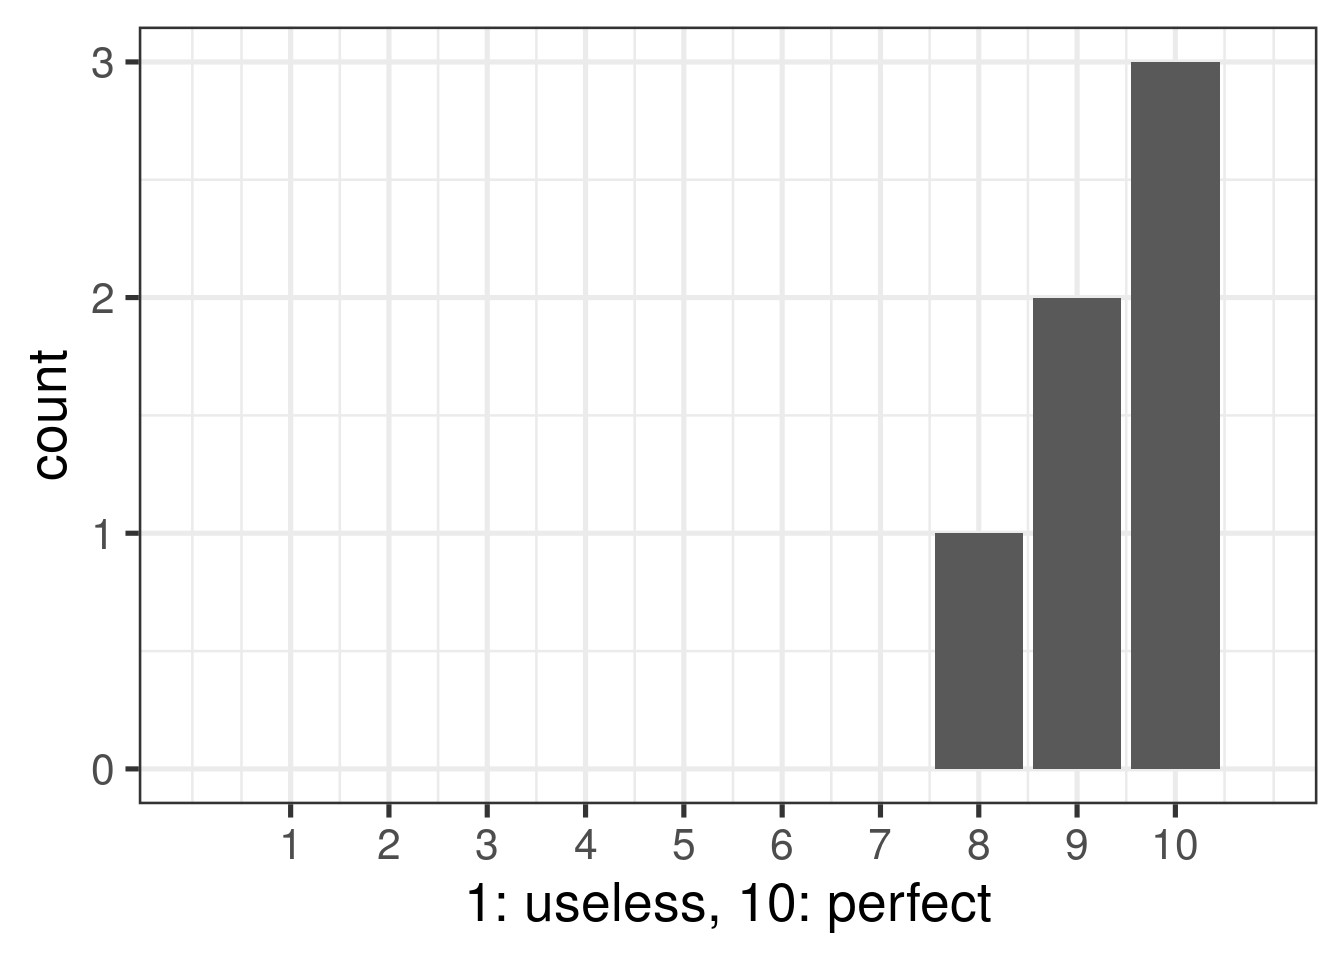
\includegraphics{_main_files/figure-latex/plot_22_2021-03-1.pdf}

\hypertarget{is-there-something-that-could-make-these-meetings-more-useful-or-productive-1}{%
\section{Is there something that could make these meetings more useful or productive?}\label{is-there-something-that-could-make-these-meetings-more-useful-or-productive-1}}

\begin{itemize}
\tightlist
\item
  I think everything is okay
\item
  My meetings with you are always very helpful.
\item
  I think the 1on1s on Monday could be a bit longer, sometimes it feels rushed and I feel bad delaying the next meeting if I have a few more things to say. I preferred having a longer and more flexible 1on1 built in to the week.
\item
  NA
\item
  Maybe an agenda
\item
  No, they are productive.
\end{itemize}

\hypertarget{do-you-think-the-current-system-of-formal-scheduled-weekly-one-on-one-meetings-is-working-should-these-be-less-frequent-more-frequent-or-stay-as-is-1}{%
\section{Do you think the current system of formal scheduled weekly one-on-one meetings is working? Should these be less frequent, more frequent, or stay as is?}\label{do-you-think-the-current-system-of-formal-scheduled-weekly-one-on-one-meetings-is-working-should-these-be-less-frequent-more-frequent-or-stay-as-is-1}}

\begin{itemize}
\tightlist
\item
  The current system is good.
\item
  Yes and maybe paired analysis sessions would be good
\item
  As is is fine, might like more time but I could request it on Calendly
\item
  I think once a week is a good frequency
\item
  I think weekly is good.
\item
  It works and I really like this system. I think it should stay as it is.
\end{itemize}

\hypertarget{do-you-think-you-would-benefit-from-more-formal-feedback-on-your-progress-1}{%
\section{Do you think you would benefit from more formal feedback on your progress?}\label{do-you-think-you-would-benefit-from-more-formal-feedback-on-your-progress-1}}

\begin{itemize}
\tightlist
\item
  No
\item
  Yes
\item
  Yes
\item
  Yes, if possible, though it doesn't need to be formal.
\item
  I think the feedback I receive is excellent
\item
  Yes, especially when it comes to code in things I am learning
\end{itemize}

\hypertarget{how-supported-do-you-feel-by-me-and-do-you-think-that-you-are-getting-the-mentoring-career-advice-and-general-guidance-to-succeed-1}{%
\section{How supported do you feel by me, and do you think that you are getting the mentoring, career advice, and general guidance to succeed?}\label{how-supported-do-you-feel-by-me-and-do-you-think-that-you-are-getting-the-mentoring-career-advice-and-general-guidance-to-succeed-1}}

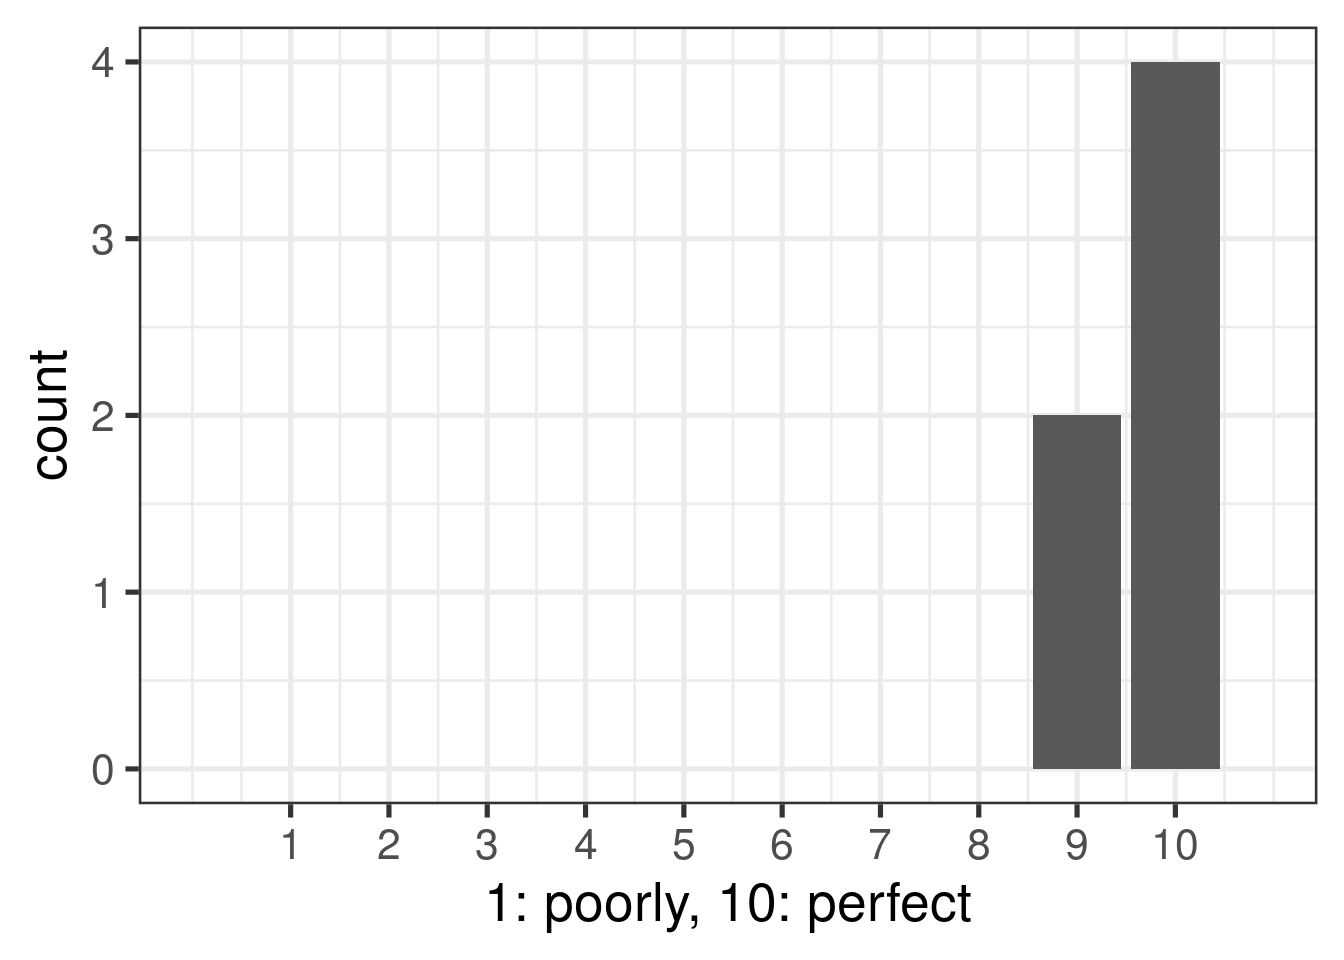
\includegraphics{_main_files/figure-latex/plot_26_2021-03-1.pdf}

\hypertarget{do-you-want-formal-training-in-giving-talks-1}{%
\section{Do you want formal training in giving talks?}\label{do-you-want-formal-training-in-giving-talks-1}}

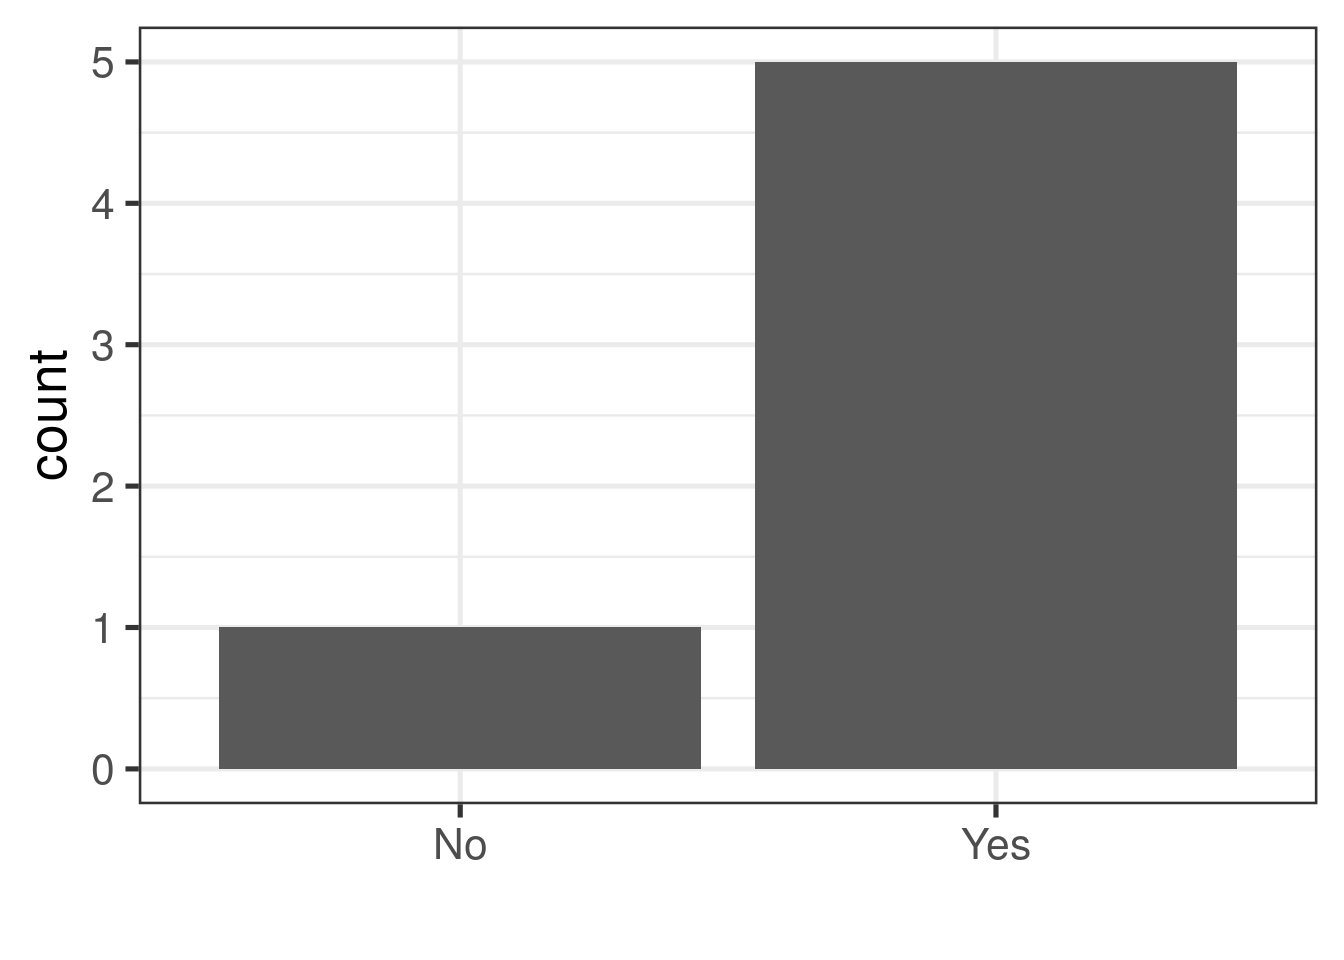
\includegraphics{_main_files/figure-latex/plot_27_2021-03-1.pdf}

\hypertarget{do-you-want-to-have-an-annual-mentoring-meeting-to-go-over-your-individual-development-plan-and-discuss-post-phd-or-post-postdoc-plans-leo-edit-see-httpslcolladotor.github.iobioc_team_dscareer-growth.html.-1}{%
\section{\texorpdfstring{Do you want to have an Annual Mentoring Meeting to go over your Individual Development Plan and discuss post-PhD or post-Postdoc plans? Leo edit: see \url{https://lcolladotor.github.io/bioc_team_ds/career-growth.html}.}{Do you want to have an Annual Mentoring Meeting to go over your Individual Development Plan and discuss post-PhD or post-Postdoc plans? Leo edit: see https://lcolladotor.github.io/bioc\_team\_ds/career-growth.html.}}\label{do-you-want-to-have-an-annual-mentoring-meeting-to-go-over-your-individual-development-plan-and-discuss-post-phd-or-post-postdoc-plans-leo-edit-see-httpslcolladotor.github.iobioc_team_dscareer-growth.html.-1}}

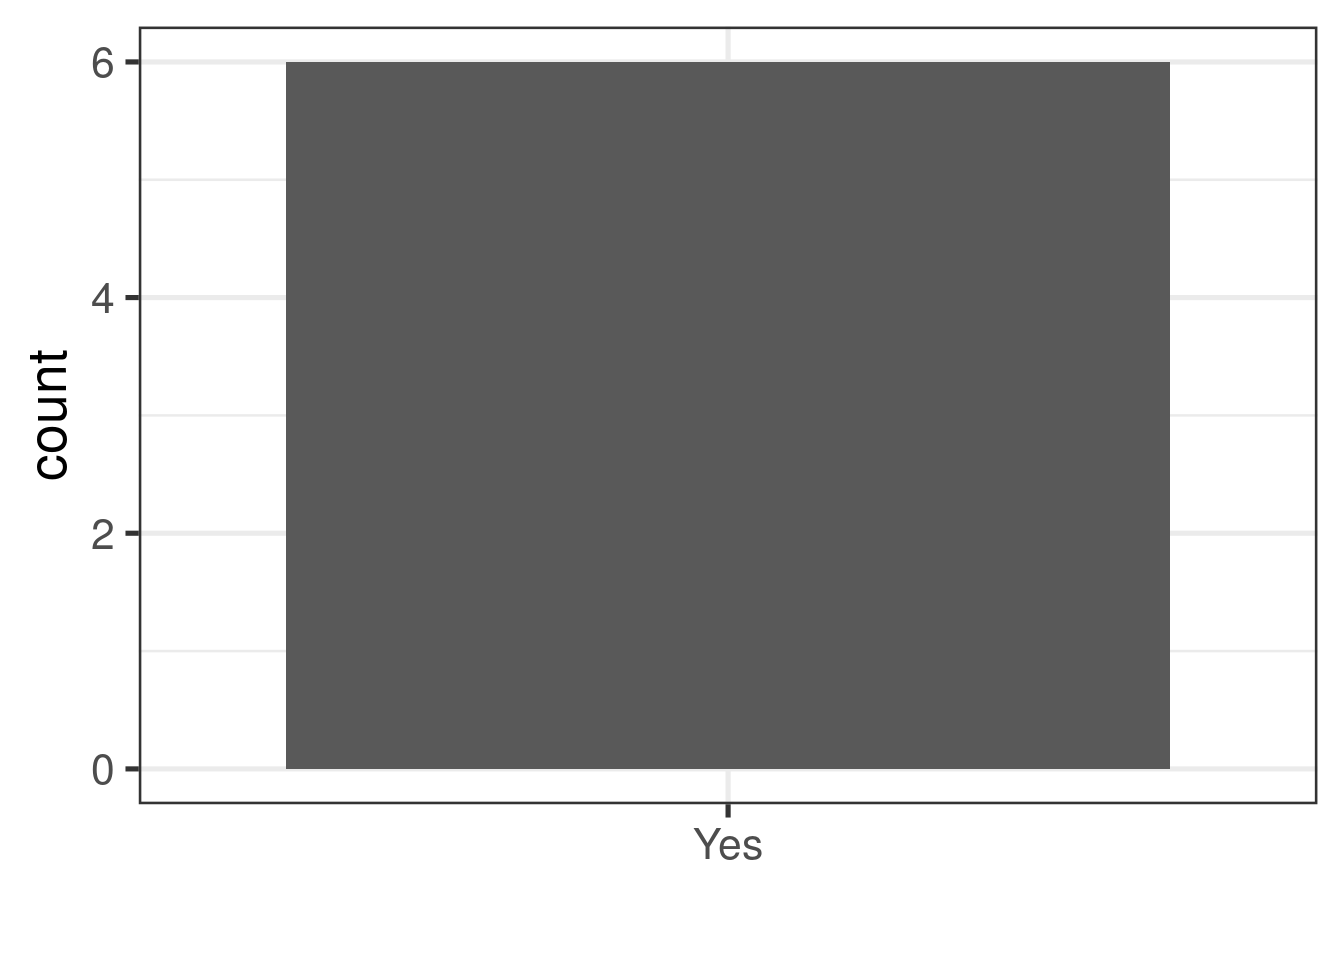
\includegraphics{_main_files/figure-latex/plot_28_2021-03-1.pdf}

\hypertarget{what-kind-of-advice-or-information-would-be-useful-to-discuss-at-such-an-annual-mentoring-meeting-1}{%
\section{What kind of advice or information would be useful to discuss at such an Annual Mentoring Meeting?}\label{what-kind-of-advice-or-information-would-be-useful-to-discuss-at-such-an-annual-mentoring-meeting-1}}

\begin{itemize}
\tightlist
\item
  Skills that need to be learned. Areas of weakness that need to be improved.
\item
  Career goals \& next steps at LIBD. Potential opportunities (projects, talks, ect.)
\item
  How to apply to phd programs. Leo and I have already talked about this.
\item
  Our current annual meetings are formatted well.
\item
  NA
\item
  How to get promoted
\end{itemize}

\hypertarget{do-you-have-any-explicit-feedback-on-how-i-can-improve-my-mentoring-style-1}{%
\section{Do you have any explicit feedback on how I can improve my mentoring style?}\label{do-you-have-any-explicit-feedback-on-how-i-can-improve-my-mentoring-style-1}}

\begin{itemize}
\tightlist
\item
  No
\item
  Probably a little more structure in terms of expectations around progress and deadlines.
\item
  NA
\item
  The current style is very good.
\item
  I think you're a great mentor.
\item
  Not really
\end{itemize}

\hypertarget{do-you-feel-it-is-easy-to-get-information-from-me-1}{%
\section{Do you feel it is easy to get information from me?}\label{do-you-feel-it-is-easy-to-get-information-from-me-1}}

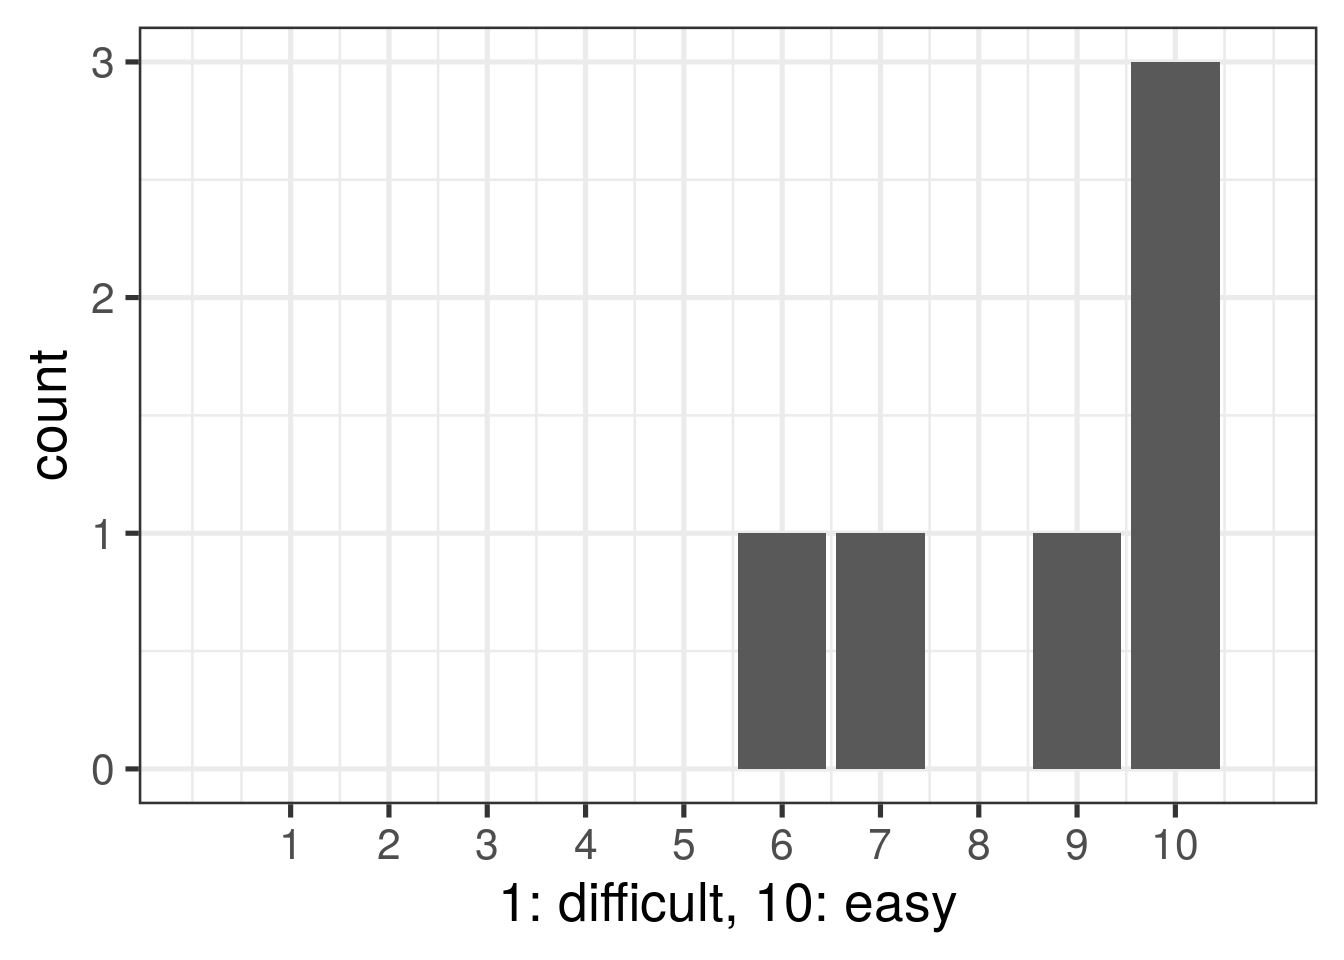
\includegraphics{_main_files/figure-latex/plot_31_2021-03-1.pdf}

\hypertarget{do-you-feel-it-is-easy-to-get-information-from-other-people-in-the-team-1}{%
\section{Do you feel it is easy to get information from other people in the team?}\label{do-you-feel-it-is-easy-to-get-information-from-other-people-in-the-team-1}}

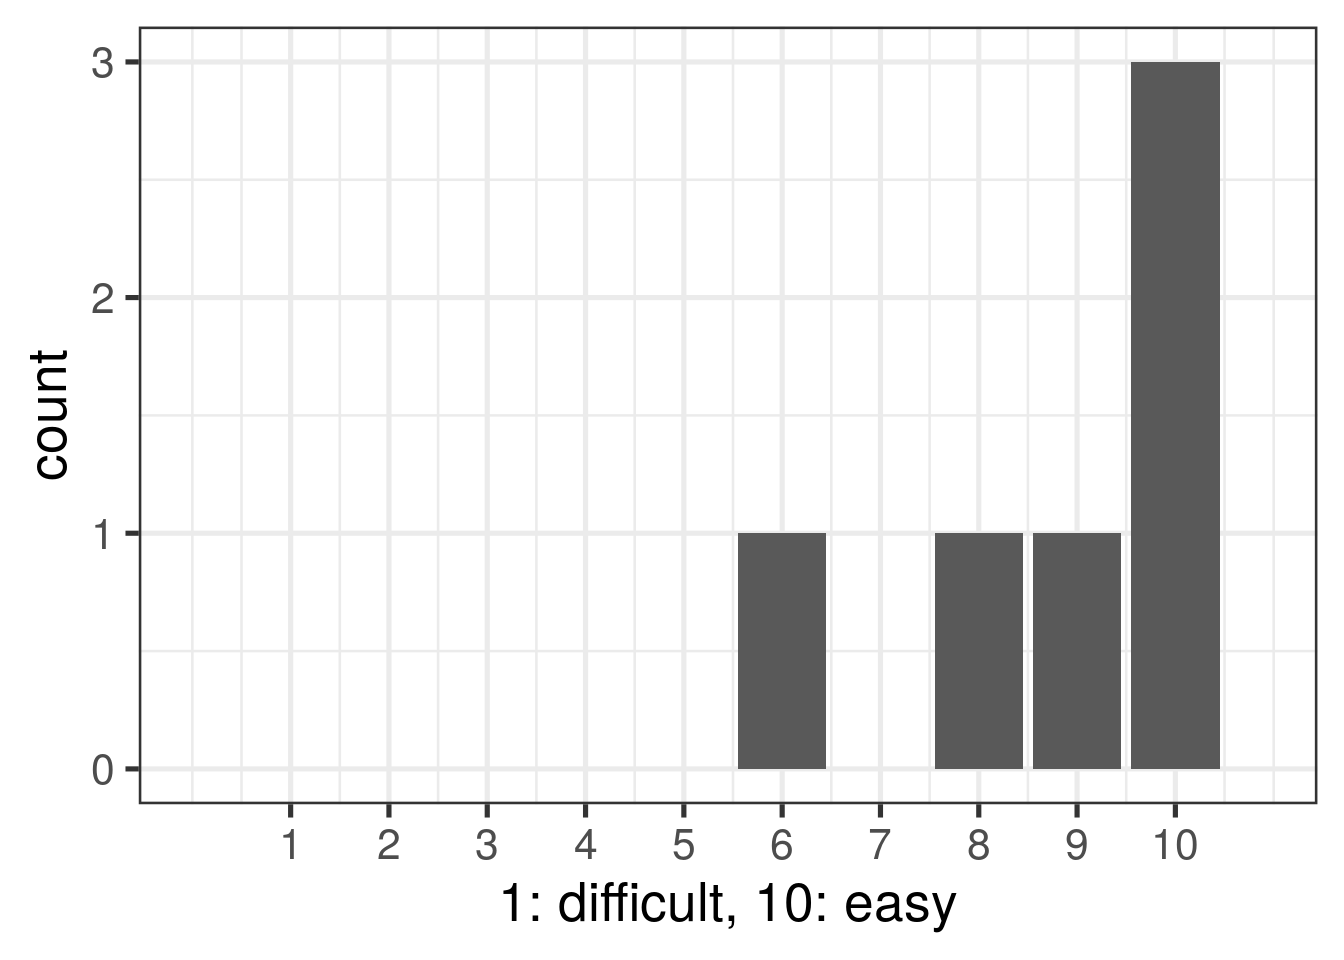
\includegraphics{_main_files/figure-latex/plot_32_2021-03-1.pdf}

\hypertarget{how-useful-do-you-find-team-meetings-1}{%
\section{How useful do you find team meetings?}\label{how-useful-do-you-find-team-meetings-1}}

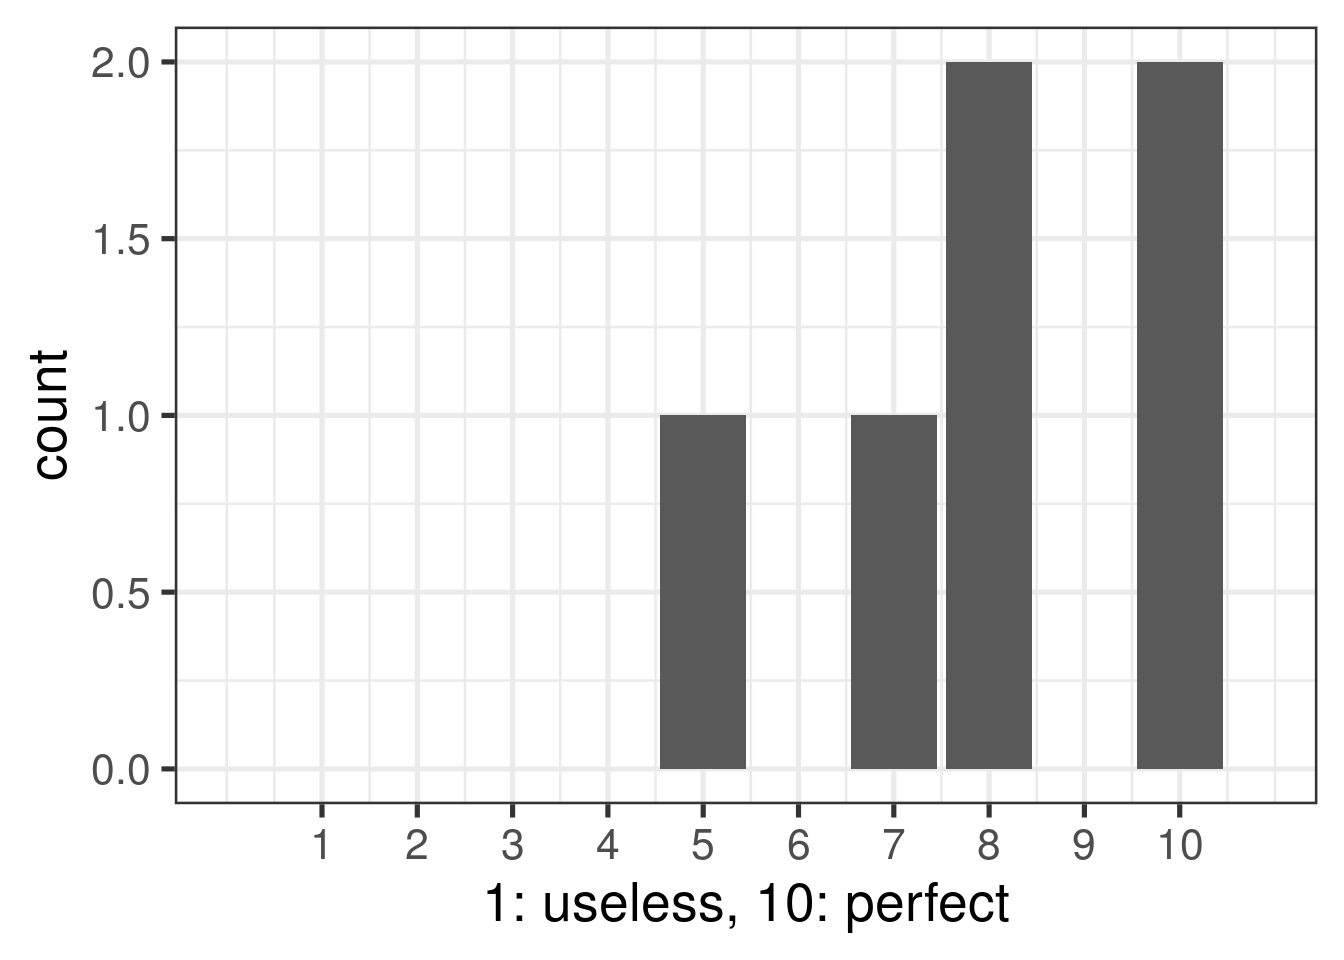
\includegraphics{_main_files/figure-latex/plot_33_2021-03-1.pdf}

\hypertarget{is-there-something-that-could-make-team-meetings-more-useful-or-productive-1}{%
\section{Is there something that could make team meetings more useful or productive?}\label{is-there-something-that-could-make-team-meetings-more-useful-or-productive-1}}

\begin{itemize}
\tightlist
\item
  We could maybe focus more on problems we encounter/ are working on during the week.
\item
  Maybe a scheduled agenda
\item
  I think our meetings are very productive.
\item
  No
\item
  It's nice to hear what everyone is up to in their individual projects, but its not always useful (it can be easy to check out). Maybe we could make the Notion board more of a part of it? Do a number rundown (we put up x number of tasks to do and got y done). It can be easy to forget the Notion board since we don't really engage with it at meetings. My favorite part of the when everyone gets chatting about a subject work related or not.
\item
  they're more or less fine as-is. The only thing I can think of that could be useful is having someone take meeting notes, so we know what was covered. Not urgent though.
\end{itemize}

\hypertarget{how-useful-do-you-find-sub-group-meetings-1}{%
\section{How useful do you find sub-group meetings?}\label{how-useful-do-you-find-sub-group-meetings-1}}

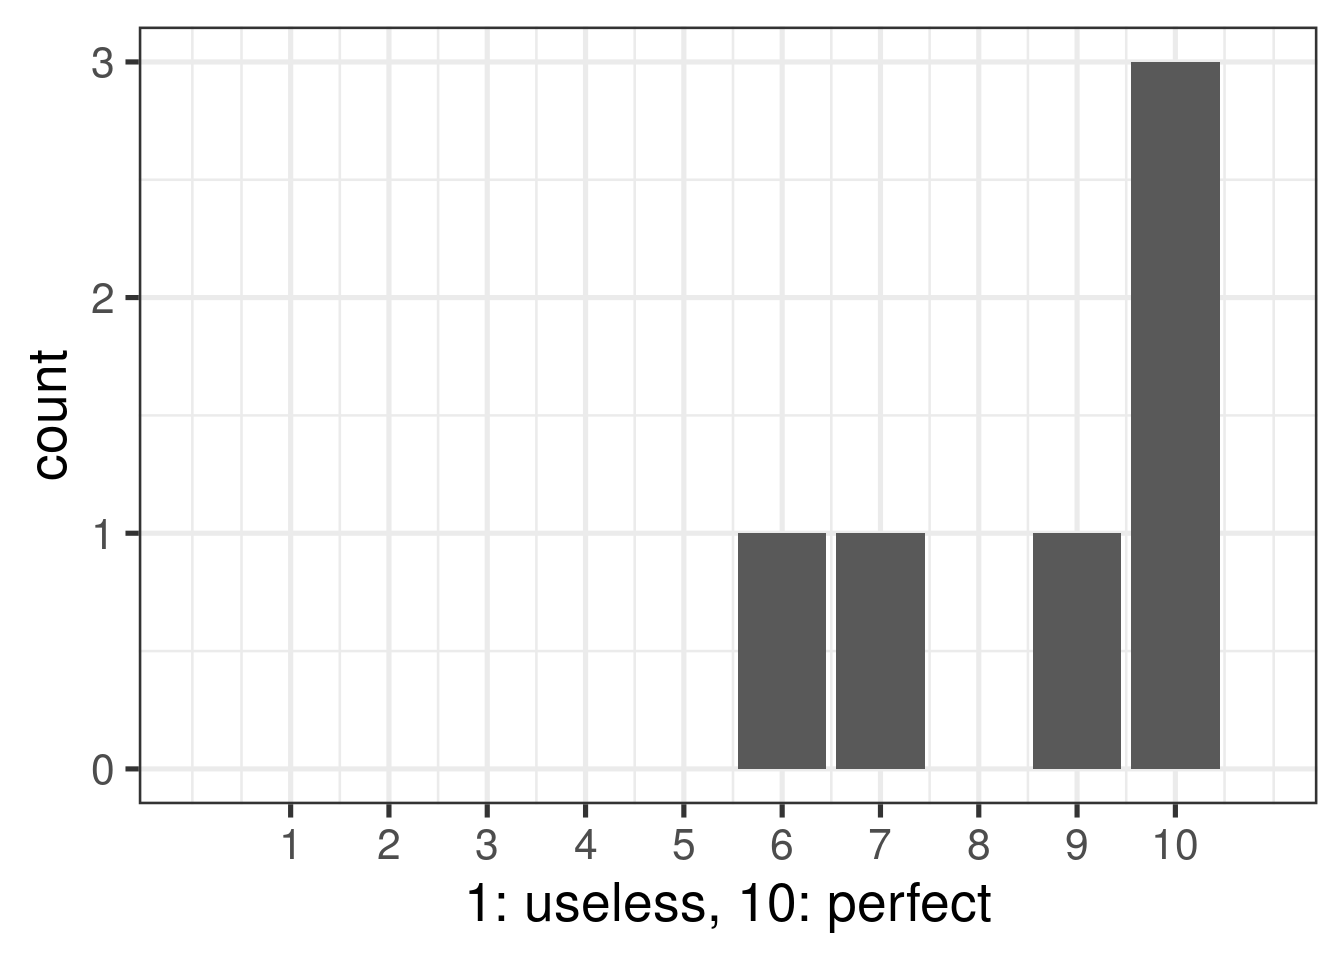
\includegraphics{_main_files/figure-latex/plot_35_2021-03-1.pdf}

\hypertarget{is-there-something-that-could-make-sub-group-meetings-more-useful-or-productive-1}{%
\section{Is there something that could make sub-group meetings more useful or productive?}\label{is-there-something-that-could-make-sub-group-meetings-more-useful-or-productive-1}}

\begin{itemize}
\tightlist
\item
  No
\item
  No.
\item
  No
\item
  I find meetings focused on one topic or goal to be the most productive, maybe make a conscious effort to record what progress/decisions were made on slack
\item
  N/A
\item
  not entirely sure what a sub-group meeting is but if it's a meeting on a project or topic then I think they're fine as-is - maybe delegating note-taking would be and having a formal agenda after each meeting
\end{itemize}

\hypertarget{how-useful-do-you-find-the-journal-club-1}{%
\section{How useful do you find the journal club?}\label{how-useful-do-you-find-the-journal-club-1}}

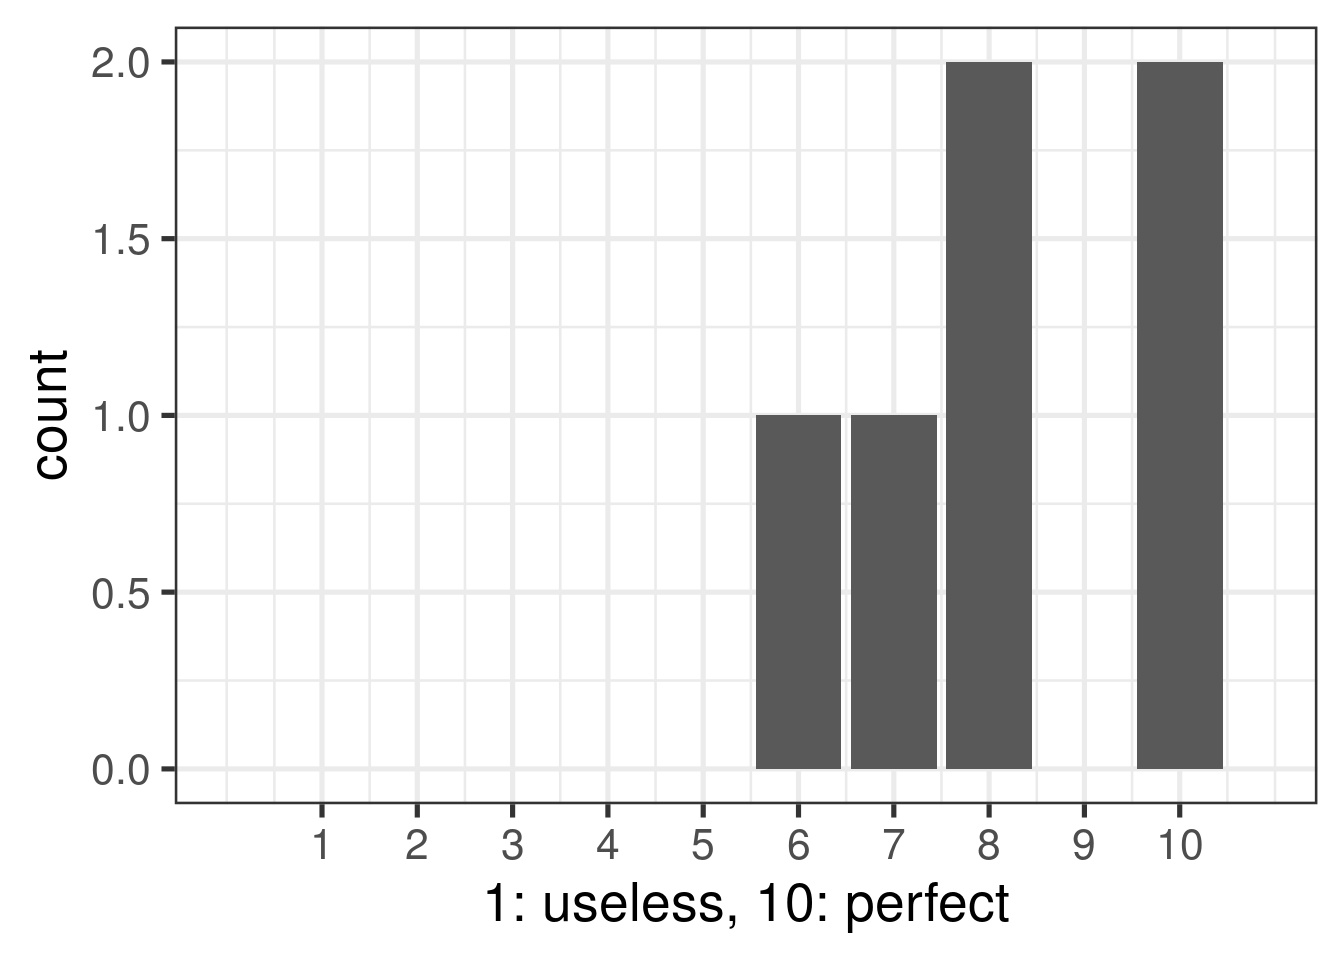
\includegraphics{_main_files/figure-latex/plot_37_2021-03-1.pdf}

\hypertarget{is-there-something-that-could-make-the-journal-club-more-useful-or-productive-1}{%
\section{Is there something that could make the journal club more useful or productive?}\label{is-there-something-that-could-make-the-journal-club-more-useful-or-productive-1}}

\begin{itemize}
\tightlist
\item
  some sort of shared repository for notes, or summary
\item
  more accountability to read the article. I feel it's not as interactive as it could be.
\item
  I find the journal club most useful when I am the one presenting because it forces me to learn a paper. If the paper someone else is presenting is too long or specific it can be hard to engage with it. Maybe more guidance on topics/how to find papers good for the club?
\item
  No.
\item
  No
\item
  Sometimes journal club is on topics that are very far outside my realm of knowledge and the work I do. But that's ok because I get to learn about new things.
\end{itemize}

\hypertarget{how-much-freedom-do-you-feel-you-have-to-decide-how-you-do-your-work-1}{%
\section{How much freedom do you feel you have to decide how you do your work?}\label{how-much-freedom-do-you-feel-you-have-to-decide-how-you-do-your-work-1}}

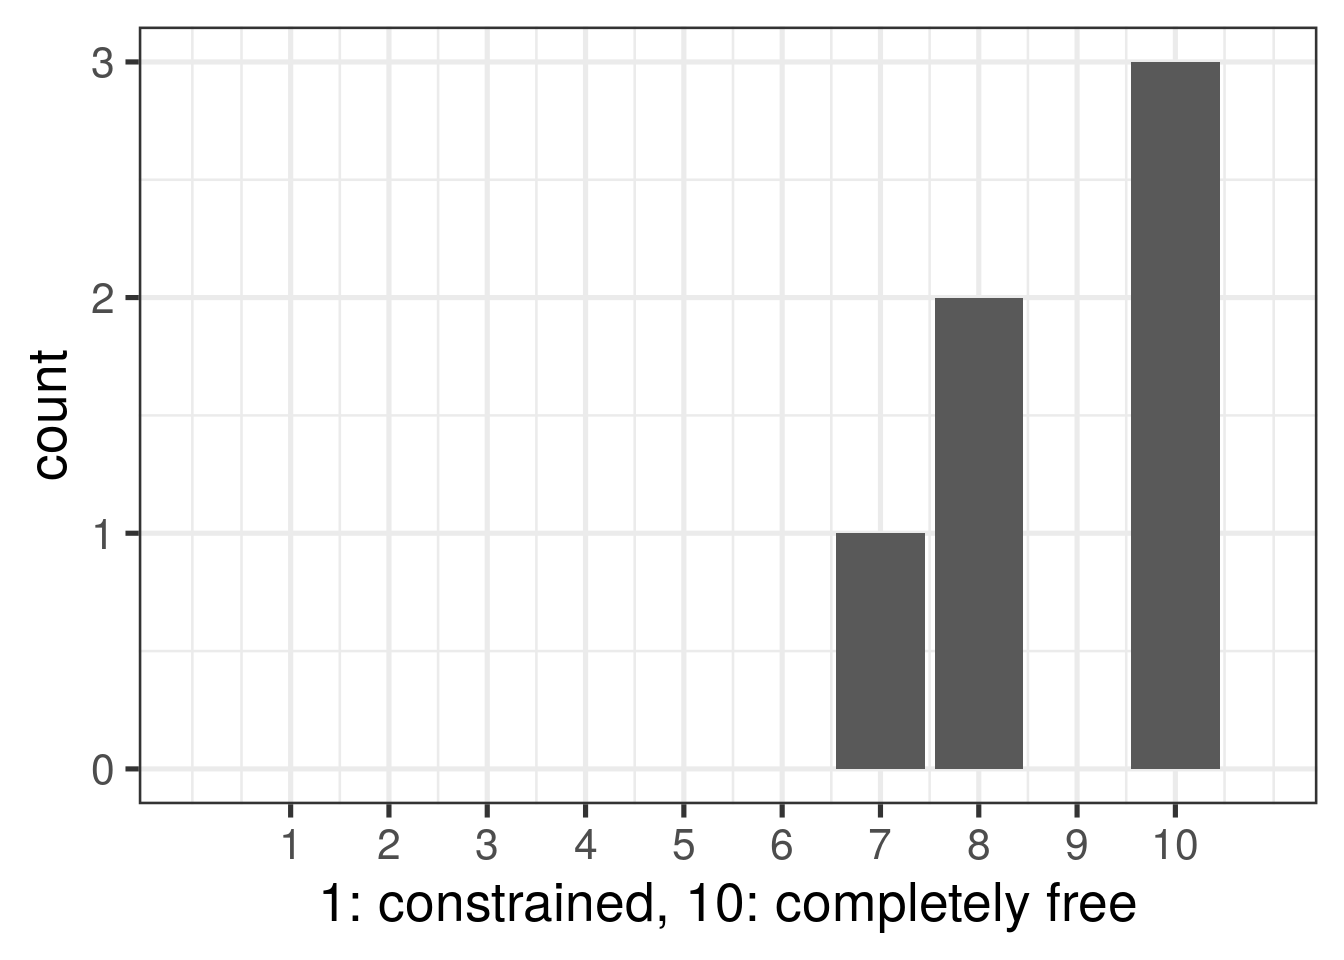
\includegraphics{_main_files/figure-latex/plot_39_2021-03-1.pdf}

\hypertarget{how-collaborative-do-you-think-the-team-is-1}{%
\section{How collaborative do you think the team is?}\label{how-collaborative-do-you-think-the-team-is-1}}

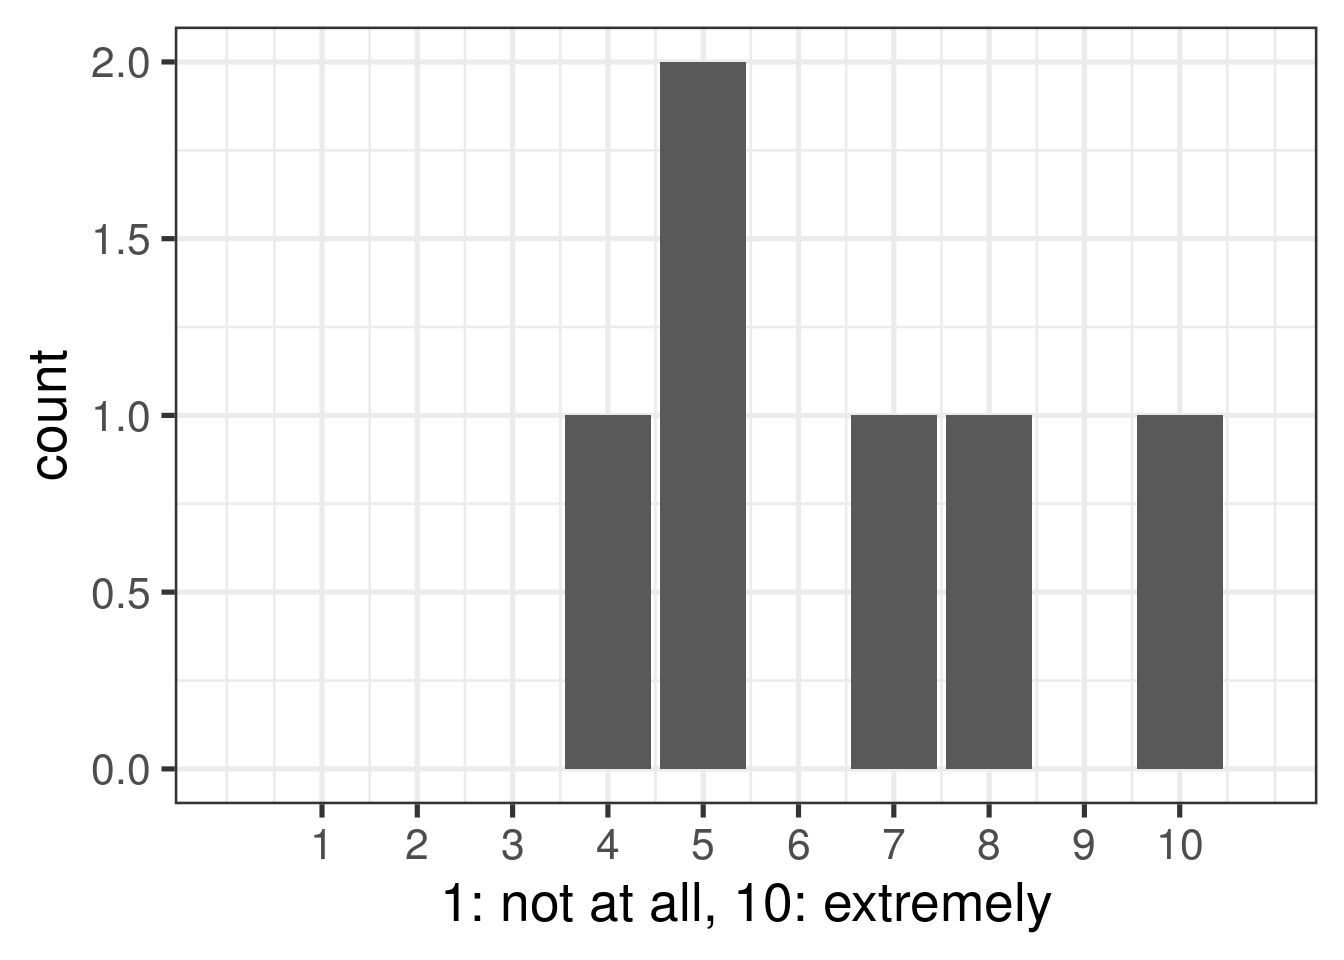
\includegraphics{_main_files/figure-latex/plot_40_2021-03-1.pdf}

\hypertarget{do-you-perceive-that-there-is-any-favoritism-in-the-team-please-elaborate.-1}{%
\section{Do you perceive that there is any favoritism in the team? Please elaborate.}\label{do-you-perceive-that-there-is-any-favoritism-in-the-team-please-elaborate.-1}}

\begin{itemize}
\tightlist
\item
  none whatsoever
\item
  No
\item
  No
\item
  No.
\item
  No
\item
  no
\end{itemize}

\hypertarget{are-there-any-issues-with-collaborations-in-the-team-that-are-not-working-please-explain.-1}{%
\section{Are there any issues with collaborations in the team that are not working? Please explain.}\label{are-there-any-issues-with-collaborations-in-the-team-that-are-not-working-please-explain.-1}}

\begin{itemize}
\tightlist
\item
  No.
\item
  No
\item
  This has gotten better recently but I feel like collaborations do not happen all that often
\item
  No
\item
  no
\item
  I feel good about the projects I am collaborating with others on
\end{itemize}

\hypertarget{are-you-aware-of-the-teams-authorship-policies-1}{%
\section{Are you aware of the team's authorship policies?}\label{are-you-aware-of-the-teams-authorship-policies-1}}

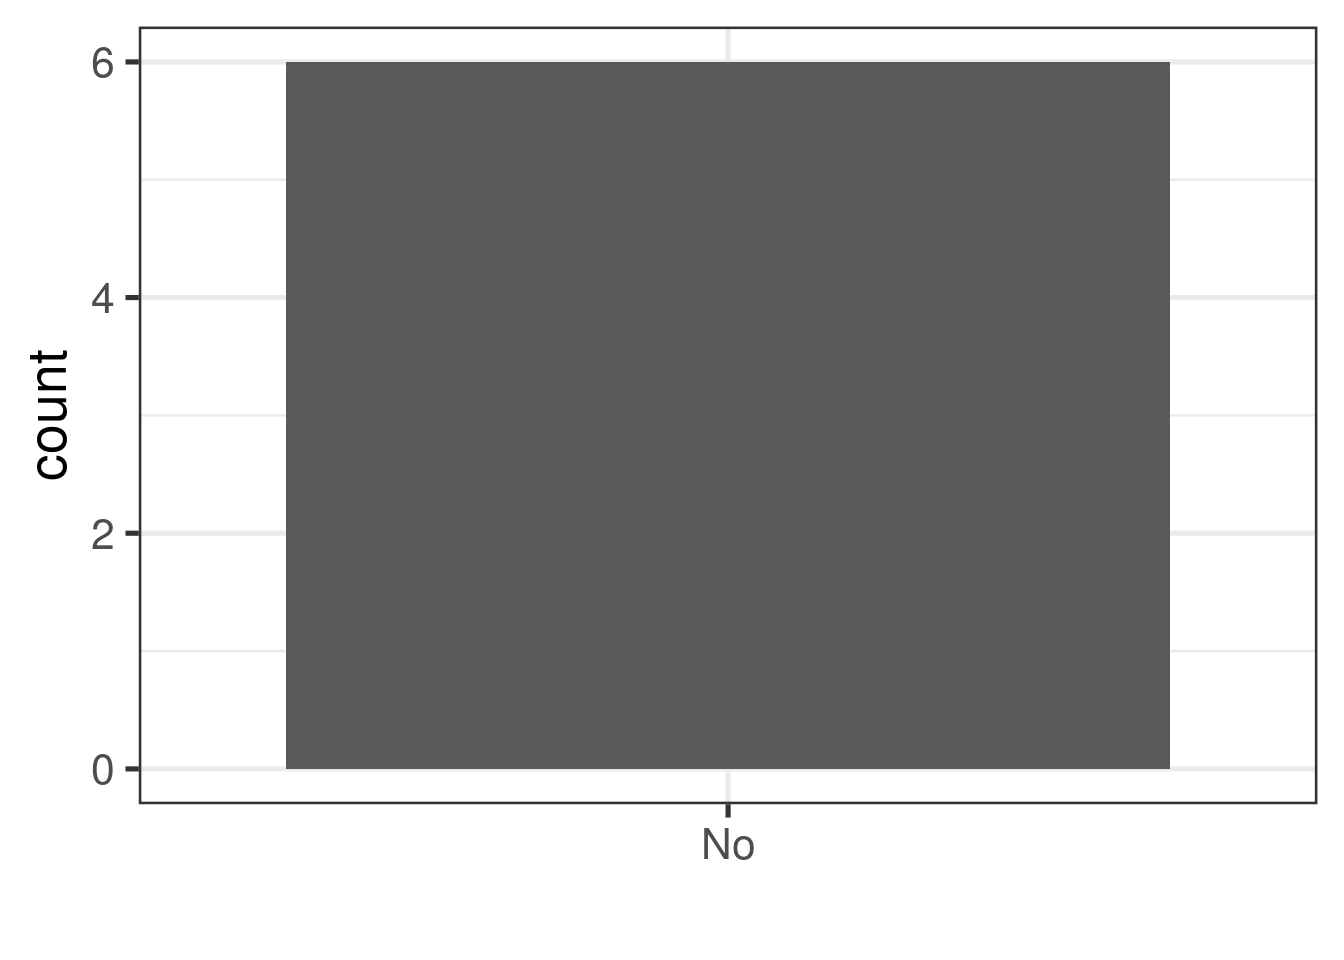
\includegraphics{_main_files/figure-latex/plot_43_2021-03-1.pdf}

\hypertarget{do-have-any-concerns-about-anticipated-authorship-on-papers-describing-your-work-or-collaborations-that-you-are-involved-with-1}{%
\section{Do have any concerns about anticipated authorship on papers describing your work or collaborations that you are involved with?}\label{do-have-any-concerns-about-anticipated-authorship-on-papers-describing-your-work-or-collaborations-that-you-are-involved-with-1}}

\begin{itemize}
\tightlist
\item
  There needs to be upfront discussions with the labs we collaborate with about authorship
\item
  No
\item
  No
\item
  No, but authorship hasn't always been explicitly discussed.
\item
  no
\item
  No
\end{itemize}

\hypertarget{please-rate-whether-you-feel-the-team-provides-you-with-the-tools-and-technologies-you-need-1}{%
\section{Please rate whether you feel the team provides you with the tools and technologies you need?}\label{please-rate-whether-you-feel-the-team-provides-you-with-the-tools-and-technologies-you-need-1}}

\includegraphics{_main_files/figure-latex/plot_45_2021-03-1.pdf}

\hypertarget{do-you-feel-you-have-received-proper-training-to-perform-the-techniques-required-for-your-work-1}{%
\section{Do you feel you have received proper training to perform the techniques required for your work?}\label{do-you-feel-you-have-received-proper-training-to-perform-the-techniques-required-for-your-work-1}}

\begin{itemize}
\tightlist
\item
  Yes, and if I feel shaky on something I feel comfortable asking questions
\item
  Yes.
\item
  yes
\item
  Yes
\item
  More-or-less - could use more detailed background information/notes/history when taking over projects that are already partially completed
\item
  Yes
\end{itemize}

\hypertarget{is-there-further-training-you-would-like-to-receive-to-help-you-accomplish-your-goals-1}{%
\section{Is there further training you would like to receive to help you accomplish your goals?}\label{is-there-further-training-you-would-like-to-receive-to-help-you-accomplish-your-goals-1}}

\begin{itemize}
\tightlist
\item
  Support in establishing a fully voluntary book club would be cool. Like a fully-optional bioinformatics ``class.'' Rstats Club is good but I feel like they are one-off lessons that don't accumulate over time the same way a book club would.
\item
  Get more in-depth building R packages, get more confident doing statistics
\item
  Yes
\item
  No
\item
  Opportunity to attend conferences provides that well enough.
\item
  More data science training
\end{itemize}

\hypertarget{how-easy-is-it-easy-to-locate-things-in-at-jhpce-github-1}{%
\section{How easy is it easy to locate things in at JHPCE / GitHub?}\label{how-easy-is-it-easy-to-locate-things-in-at-jhpce-github-1}}

\includegraphics{_main_files/figure-latex/plot_48_2021-03-1.pdf}

\hypertarget{how-often-do-you-encounter-issues-that-could-have-been-averted-if-things-were-better-organized-e.g.-missing-readme-or-github-repository.-1}{%
\section{How often do you encounter issues that could have been averted if things were better organized? E.g. missing README or GitHub repository.}\label{how-often-do-you-encounter-issues-that-could-have-been-averted-if-things-were-better-organized-e.g.-missing-readme-or-github-repository.-1}}

\includegraphics{_main_files/figure-latex/plot_49_2021-03-1.pdf}

\hypertarget{please-tell-me-more-about-the-kinds-of-organizational-issues-you-have-encountered-and-any-suggestions-to-improve-such-issues.-1}{%
\section{Please tell me more about the kinds of organizational issues you have encountered and any suggestions to improve such issues.}\label{please-tell-me-more-about-the-kinds-of-organizational-issues-you-have-encountered-and-any-suggestions-to-improve-such-issues.-1}}

\begin{itemize}
\tightlist
\item
  Sometimes I get handed scripts to use as examples and I have a hard time finding the data objects that the scripts are using. Or I have a hard time finding the output of the scripts.
\item
  Mostly just messy directories and filenames. I like the move to ``by-grant'' organization on JHPCE.
\item
  I have not encountered any issue
\item
  NA
\item
  still need improvement on interactions with broader institute.
\item
  Others' code is often not documented, or context for performing certain code does not exist.
\end{itemize}

\hypertarget{what-is-your-opinion-of-the-level-of-technical-support-in-the-team-1}{%
\section{What is your opinion of the level of technical support in the team?}\label{what-is-your-opinion-of-the-level-of-technical-support-in-the-team-1}}

\includegraphics{_main_files/figure-latex/plot_51_2021-03-1.pdf}

\hypertarget{what-is-your-opinion-of-the-level-of-administrative-support-in-the-team-1}{%
\section{What is your opinion of the level of administrative support in the team?}\label{what-is-your-opinion-of-the-level-of-administrative-support-in-the-team-1}}

\includegraphics{_main_files/figure-latex/plot_52_2021-03-1.pdf}

\hypertarget{what-is-your-impression-of-the-funding-of-the-team-1}{%
\section{What is your impression of the funding of the team?}\label{what-is-your-impression-of-the-funding-of-the-team-1}}

\includegraphics{_main_files/figure-latex/plot_53_2021-03-1.pdf}

\hypertarget{if-we-had-the-funds-to-hire-one-more-full-time-person-what-kind-of-person-should-we-hire-and-what-role-would-they-play-in-the-team-1}{%
\section{If we had the funds to hire one more full-time person, what kind of person should we hire and what role would they play in the team?}\label{if-we-had-the-funds-to-hire-one-more-full-time-person-what-kind-of-person-should-we-hire-and-what-role-would-they-play-in-the-team-1}}

\begin{itemize}
\tightlist
\item
  I'm not sure what is needed.
\item
  Someone who has strong R and or python skills and has studied/and experience in bioinformatics. As for role, more analysis work (idk this is a hard one to answer)
\item
  A math-y person to help explain the type of statistics we use.
\item
  I feel like someone to take some of the pressure off your load would be helpful to the team. You seem very busy and sometimes it would be nice to have someone with about your level of knowledge and experience (or even slightly less) to consult about certain issues.
\item
  Staff scientist level/post-doc would be perfect
\item
  I'm not sure about that
\end{itemize}

\hypertarget{is-there-something-that-you-experienced-in-a-previous-job-that-you-wish-we-also-did-here-1}{%
\section{Is there something that you experienced in a previous job that you wish we also did here?}\label{is-there-something-that-you-experienced-in-a-previous-job-that-you-wish-we-also-did-here-1}}

\begin{itemize}
\tightlist
\item
  Absolutely not
\item
  No.
\item
  No
\item
  Raises
\item
  Team meeting where people presented one slide (usually a graph) of what they did on their project that week
\item
  NA
\end{itemize}

\hypertarget{are-there-any-concerns-or-other-areas-of-the-team-you-believe-could-be-improved-that-have-not-been-addressed-in-previous-questions-please-list-any-other-areas-you-think-could-be-improved-or-should-be-addressed.-1}{%
\section{Are there any concerns or other areas of the team you believe could be improved that have not been addressed in previous questions? Please list any other areas you think could be improved or should be addressed.}\label{are-there-any-concerns-or-other-areas-of-the-team-you-believe-could-be-improved-that-have-not-been-addressed-in-previous-questions-please-list-any-other-areas-you-think-could-be-improved-or-should-be-addressed.-1}}

\begin{itemize}
\tightlist
\item
  Returning to the lab expirations and timeline
\item
  NA
\item
  My only concern at the institute is that sometimes the amount of information on slack can be overwhelming.
\item
  No
\item
  No
\item
  No.
\end{itemize}

\hypertarget{finally-did-you-find-this-survey-useful-if-yes-how-often-should-the-survey-be-conducted-1}{%
\section{Finally, did you find this survey useful? If yes, how often should the survey be conducted?}\label{finally-did-you-find-this-survey-useful-if-yes-how-often-should-the-survey-be-conducted-1}}

\begin{itemize}
\tightlist
\item
  The survey is good and could be conducted annually. Some of the 1-10 questions could confuse people wo don't read the question well enough on their initial read (like me), because they use the 10-end of the scale to represent a lower magnitude of something bad (like `Not pressured') and the 1-end of the scale to represent a higher magnitude of something bad (like `Very pressured'). Ultimately not a problem for me because I re-read the scale labels but this might cause some erroneous answers.
\item
  Somewhat. This could maybe be a yearly thing (or a couple times a year).
\item
  It was useful, but it was a bit long. I think yearly for something this long, maybe something more concise if we would do it with more frequency. Also in a group this small I feel like it is only so anonymous and we have a lot of discussions about this kind of stuff as a group already.\\
\item
  Yes, maybe every 6 months.
\item
  Yes
\item
  Yes
\end{itemize}

\end{document}
